%\RequirePackage{kvoptions-patch}	% required, do not delete 
% --> not compatible with newer miktex versions, restriction on spelling keys and keyvalues 
\documentclass[
	language=en ,        	% choose between "de" or "en"
	layout=twoside ,		% chose between "oneside" or "twoside"
	titlepage=true ,		% include titlepage(s) (true) or not (false)
	preamble=true ,			% include preamble (optional)
	draftmode=false ,		% enable (true) or disable (false) draft mode
]{sbmthesis}
\setlength\headheight{30pt} % required, do not delete
\pdfminorversion=7

% +-----------------------------------------------------------------------------+
% | Die Kopfseiten der Arbeit werden kurz vor Abgabe vom Betreuer ausgehändigt. |
% +-----------------------------------------------------------------------------+

% +----------------------------+
% | Add hyphenation rules here |
% +----------------------------+
\hyphenation{
    % In some special cases LaTeX is unable to correctly hyphenate a term. Thus 		you have to define a custom hypenation rule here using minus signs. This is 		the case when a term overlaps with the page margins. Separate multiple 				entries with white space.
    % Examples: Doppel-kupplungs-ge-triebe Kupp-lungs-schlupf-reg-ler
}

% +-----------------------------------------------------+
% | 			Include other packages here 			|
% |							or 							|
% | at the intended position in the cls file (prefered) |
% +-----------------------------------------------------+
\usepackage{rotating}
\usepackage{pgfgantt}
\usepackage{xcolor}
\usepackage{listings}
\usepackage{amssymb}
\usepackage{float}
\definecolor{NavyBlue}{rgb}{0.0, 0.0, 0.5}
\definecolor{gray50}{gray}{0.5}
\lstset{
    language=SQL,
    basicstyle=\ttfamily,
    keywordstyle=\color{blue}\bfseries,
    commentstyle=\color{gray},
    stringstyle=\color{red},
    showstringspaces=false,
    breaklines=true
}
\lstdefinelanguage{CSharp}{
  morekeywords={abstract, as, base, bool, break, byte, case, catch, char, checked, class, const, continue, decimal, default, delegate, do, double, else, enum, event, explicit, extern, false, finally, fixed, float, for, foreach, goto, if, implicit, in, int, interface, internal, is, lock, long, namespace, new, null, object, operator, out, override, params, private, protected, public, readonly, ref, return, sbyte, sealed, short, sizeof, stackalloc, static, string, struct, switch, this, throw, true, try, typeof, uint, ulong, unchecked, unsafe, ushort, using, virtual, void, volatile, while},
  sensitive=true,
  morecomment=[l]{//},
  morecomment=[s]{/*}{*/},
  morestring=[b]",
  morestring=[b]'
}

% +-----------------------+
% | Start of the document |
% +-----------------------+
\begin{document}   
    \preliminaries
    
    % +----------------------------+
    % | Include your chapters here |
    % +----------------------------+
    % Insert \cleardoublepage after every include
    \chapter{Introduction}
\label{chap:introduction}

Modern commercial vehicles represent a quintessential example of cyber-physical systems, where sophisticated software enables precise control over complex mechanical components. The software controlling these vehicles has grown exponentially in complexity over recent decades, evolving from simple engine management to comprehensive control of virtually all vehicle functions. At the core of this evolution is the Electronic Control Unit (ECU)—a specialized computer that executes software to manage specific vehicle functions \cite{broy2006challenges}. Contemporary commercial vehicles contain dozens of interconnected ECUs working in concert to ensure optimal performance, efficiency, and safety across diverse operating conditions.

\section{Background and Context}
\label{sec:background}

The automotive industry has undergone a profound transformation over the past decades, evolving from predominantly mechanical systems to highly sophisticated mechatronic platforms \cite{pretschner2007software}. This evolution has been particularly pronounced in the commercial vehicle sector, where modern trucks rely on complex networks of Electronic Control Units to manage everything from engine performance to safety systems \cite{broy2006challenges}. These systems must adapt to a wide range of operational conditions, regulatory requirements, and market-specific configurations, creating a significant challenge in managing software variability.

At the heart of this variability management lies the Common Powertrain Controller (CPC)—a central ECU managing critical functions related to engine and transmission control. The CPC's operation is governed by thousands of configurable parameters that determine how the powertrain behaves under specific conditions \cite{staron2021automotive}. These parameters influence everything from basic engine timing to sophisticated emission control strategies, making their precise configuration essential for vehicle performance, efficiency, and regulatory compliance.

The parameter management challenge is further complicated by the global nature of modern vehicle development. Commercial vehicles must conform to different emissions regulations, operate in diverse environmental conditions, and meet varying customer expectations across global markets. Consequently, a single vehicle model may require numerous parameter configurations, each tailored to specific combinations of market requirements, hardware configurations, and customer specifications \cite{trovao2024evolution}.

\section{Problem Statement}
\label{sec:problem}

The current approach to parameter management in commercial vehicle development relies predominantly on distributed Excel spreadsheets, a methodology that emerged during a period when parameter counts were manageable and development teams were smaller \cite{trovao2024evolution}. However, as software complexity has increased exponentially, this fragmented approach has introduced significant limitations and risks to the development process.

Development teams distributed across different locations must coordinate changes to thousands of parameters, track their versions, and ensure consistency across multiple vehicle platforms. The absence of a centralized version control system makes it exceptionally difficult to track changes effectively and manage releases. This situation becomes particularly critical when dealing with safety-critical parameters that directly influence vehicle performance and regulatory compliance.

The manual nature of current processes, combined with the lack of automated validation mechanisms, introduces substantial risks of data inconsistency, version conflicts, and delayed implementation of critical parameter updates. Parameter changes are not consistently verified against established rules and constraints, potentially leading to incompatible configurations or non-compliant behavior \cite{staron2021automotive}.

Integration with critical enterprise systems presents another significant challenge. The current process of synchronizing data with internal database systems involves several manual steps, consuming valuable development resources and introducing potential points of failure in the configuration management workflow. The absence of automated data validation and synchronization mechanisms creates additional risks for data integrity and consistency across these interconnected systems.

Furthermore, the increasing emphasis on rapid development cycles and continuous integration in the automotive industry demands a more sophisticated approach to parameter management \cite{broy2006challenges}. The existing system's limitations become particularly apparent when considering the need for simultaneous development of multiple vehicle variants, each requiring specific parameter configurations for different markets and regulatory environments.

These challenges collectively underscore the urgent need for a modern, database-driven solution that can address the complexities of contemporary automotive software development while providing a scalable foundation for future growth and adaptation.

\section{Research Objectives}
\label{sec:objectives}

This thesis aims to address the fundamental challenges in automotive parameter management through the development of database architecture for VMAP (Variant Management and Parametrization), a web-based application for powertrain parameter configuration. The research objectives encompass both theoretical foundations and practical implementation considerations, focusing on creating a robust solution that meets the complex demands of modern vehicle development processes.

The primary research objective centers on developing a centralized database architecture that can effectively manage the complexity of powertrain parameters while maintaining data integrity and traceability \cite{williams2004web}. This architecture must support sophisticated version control mechanisms that can handle parameter variations across different development stages and vehicle variants. The system should provide comprehensive audit trails and change history, enabling development teams to track modifications and understand the evolution of parameter configurations over time.

A second crucial objective focuses on the implementation of a sophisticated version control system that addresses the unique requirements of parameter management in automotive software development. This system must go beyond traditional source code version control approaches to handle the complex relationships between parameters, their variants, and their applications across different vehicle platforms \cite{staron2021automotive}. The version control mechanism should support parallel development streams while maintaining consistency and preventing conflicts in parameter configurations.

The research also aims to establish a comprehensive role-based access control system that supports the diverse needs of different user groups within the development process. This includes creating specialized interfaces and permissions for Module Developers, Documentation Team members, Administrators, and Read-only Users, each with specific capabilities and restrictions aligned with their responsibilities \cite{sandhu1998role}. The access control system must balance security requirements with the need for efficient collaboration among development teams.

Integration with existing enterprise systems represents another critical objective of this research. The VMAP system must establish seamless data exchange mechanisms with internal database systems, ensuring consistent information flow while minimizing manual intervention \cite{broy2006challenges}. This integration should support automated validation of parameter changes and provide mechanisms for maintaining data consistency across different systems.

A final key objective involves the development of database interfaces and query optimization strategies that will support the web-based interface implementation. While the actual User Interface (UI) development falls outside the scope of the thesis, the research will focus on designing efficient database structures, stored procedures, and APIs that enable seamless integration with the planned web interface \cite{pretschner2007software}. This includes developing optimized query patterns for complex operations such as parameter comparison, variant management, and release workflows, while ensuring robust data validation and business rule enforcement.

\section{Significance of the Study}
\label{sec:significance}

The significance of this research extends beyond addressing immediate technical challenges in parameter management. By developing a comprehensive database solution for variant management and parametrization, this work contributes to the broader field of automotive software engineering in several important ways.

First, the research advances the understanding of version control in parameter-centric systems, extending traditional concepts of software versioning to accommodate the unique characteristics of automotive parameter configurations. While considerable research has been conducted on code versioning, the versioning of parameter data presents distinct challenges that require specialized approaches \cite{bhattacherjee2015principles}. This thesis contributes to closing this gap by developing and evaluating new methods for parameter versioning in complex automotive systems.

Second, the work addresses critical industry needs for improved quality and efficiency in vehicle development. Commercial vehicle manufacturers face increasing pressure to reduce development time while managing growing software complexity and ensuring regulatory compliance across global markets \cite{broy2006challenges}. By providing a more robust and efficient parameter management solution, this research directly contributes to these industry priorities, potentially reducing development costs and improving vehicle quality through more consistent parameter configurations.

Third, the research advances the integration of database technology with domain-specific engineering processes. By developing specialized database structures and functions tailored to the unique requirements of automotive parameter management, this work demonstrates how database technology can be adapted to support complex engineering workflows \cite{elmasri2015fundamentals}. This integration perspective is valuable not only for automotive applications but also for other engineering domains facing similar challenges in managing complex, highly variable system configurations.

Finally, the research contributes to the growing field of model-based systems engineering by providing a structured approach to managing the parametric aspects of system models. As the automotive industry continues to adopt model-based approaches for system development, the management of parameter configurations becomes increasingly critical for maintaining model integrity and traceability \cite{staron2021automotive}. This thesis provides insights and solutions that support this evolution toward more systematic model-based development practices.

\section{Thesis Structure}
\label{sec:structure}

The thesis is organized into six chapters that systematically address the research objectives and present a comprehensive solution for automotive parameter management. The structure follows a logical progression from theoretical foundations through practical implementation, ensuring thorough coverage of both academic and industry perspectives.

Following this introduction, Chapter 2 presents a comprehensive review of the state of the art in database version control systems and automotive parameter management. This chapter examines existing approaches to software configuration management in the automotive industry \cite{pretschner2007software}, analyzes current database versioning techniques \cite{bhattacherjee2015principles}, and evaluates their applicability to parameter management systems. The review encompasses both academic research and industry practices, providing a solid foundation for the proposed solution.

Chapter 3 details the methodology and concept development, beginning with a thorough requirements analysis based on industry needs and academic best practices \cite{staron2021automotive}. This chapter explores the system architecture design, consisting of the database schema, version control mechanisms, and user management frameworks. Particular attention is given to the integration requirements with existing systems and the development of robust validation mechanisms for parameter management.

The implementation strategy and technical design are presented in Chapter 4, which outlines the practical realization of the VMAP system. This chapter describes the development of the database structure, the implementation of version control mechanisms, and the creation of the database interfaces. The chapter also details the integration approaches with internal database systems, highlighting the technical challenges and solutions developed during the implementation phase \cite{broy2006challenges}.

Chapter 5 focuses on system evaluation and validation, presenting a comprehensive assessment of the VMAP system against the defined research objectives. This chapter includes detailed performance analyses, user acceptance testing results, and comparative evaluations against existing parameter management solutions. The evaluation framework incorporates both quantitative metrics and qualitative assessments to provide a thorough understanding of the system's effectiveness \cite{elmasri2015fundamentals}.

The thesis concludes with Chapter 6, which summarizes the research findings and presents recommendations for future development. This chapter reflects on the contributions of the research to both academic knowledge and industry practice, discussing the implications for automotive software development and configuration management. Additionally, it outlines potential areas for future research and system enhancement based on the insights gained during the project.

Throughout these chapters, the research methodology combines theoretical analysis with practical implementation, ensuring that the resulting system meets both academic standards and industry requirements. Special attention is given to database versioning approaches, user role management, and integration strategies with existing systems, addressing the unique challenges of automotive software configuration management \cite{staron2021automotive}.


\section{Project Plan}

The research project follows a structured approach spanning six months from November 2024 to April 2025, organized into three distinct phases: Exposé, Implementation, and Finalization. The comprehensive timeline ensures systematic progression through all research objectives while maintaining academic rigor and quality standards.

\subsection{Exposé Phase (November - January)}

The initial phase focuses on establishing strong theoretical foundations and gathering comprehensive requirements. Literature review constitutes a significant portion of this phase, extending over six weeks to ensure thorough coverage of current database versioning approaches, parameter management systems, and industry practices in automotive applications. This review encompasses analysis of existing version control systems, examination of industry standards for software configuration management, and evaluation of current parameter management solutions.

Requirements analysis follows the literature review, spanning three weeks to capture detailed system specifications. This phase involves extensive stakeholder consultation to document system requirements, analyze existing Excel-based workflows, define integration requirements with internal database systems, and establish user roles and access control specifications. The Exposé phase concludes with the submission of a comprehensive research proposal at the end of Week 3 in January.

\subsection{Implementation Phase (December - March)}

The implementation phase encompasses four major components, each allocated four weeks for development and refinement. Database design initiates this phase, focusing on developing the schema for parameter management, designing version control mechanisms, creating data models for user management, and planning integration interfaces with existing systems. 

System architecture development follows, concentrating on overall system design, version control workflows, user management frameworks, and validation mechanisms. This stage establishes the foundational structure for the entire system while ensuring alignment with identified requirements and industry standards.

Prototype development constitutes the third component, involving implementation of core database functionality, development of version control features, creation of user management interfaces, and construction of system integration components. This stage transforms theoretical designs into practical implementations while maintaining focus on system usability and performance.

The final component of this phase involves comprehensive testing and validation, including database performance testing, validation of version control mechanisms, testing of user management functions, and verification of system integration capabilities. This stage ensures all implemented features meet specified requirements and performance standards.

\subsection{Finalization Phase (April)}

The concluding phase focuses on documentation and thesis preparation over four weeks. The first two weeks are dedicated to comprehensive documentation, including compilation of implementation details and system architecture documentation. 

The subsequent two weeks concentrate on thesis writing, involving comprehensive documentation of research findings, inclusion of test results and analysis, preparation of conclusions and recommendations, and thorough content review and refinement. The phase concludes with thesis submission in Week 16 and final project presentation in Week 17.

\begin{sidewaysfigure}
        \begin{ganttchart}[vgrid,
            y unit title = 0.7cm,
            y unit chart = 0.5cm,
            bar/.append style={fill=red!70},
            bar incomplete/.append style={fill=black!30},
            bar top shift =0.2,
            bar height=.5,
            group/.append style={draw=black,fill=NavyBlue!70},
            group incomplete/.append style={draw=black, fill=black!50},
            group left shift=0,
            group right shift=0,
            group height=.7,
            group peaks height = 0,
            milestone height = 0.7,
            milestone/.append style={fill=orange},
            ]{1}{25}
            
            \gantttitle{2024-2025}{25} \\
            \gantttitle{Nov}{4}\gantttitle{Dec}{4}\gantttitle{Jan}{5}\gantttitle{Feb}{4}\gantttitle{Mar}{4}\gantttitle{Apr}{4} \\
            \gantttitlelist{45,...,52}{1}
            \gantttitlelist{1,...,17}{1} \\
            
            \ganttgroup{Exposé}{1}{7} \\
            \ganttbar{Literature Review}{1}{6} \\
            \ganttbar{Requirements Analysis}{3}{5} \\
            \ganttmilestone{Exposé Submission}{11} \\
            
            \ganttgroup{Implementation}{5}{21} \\
            \ganttbar{Database Design}{5}{8} \\
            \ganttlinkedbar{System Architecture}{9}{12} \\
            \ganttlinkedbar{Prototype Development}{13}{17} \\
            \ganttlinkedbar{Testing and Validation}{18}{21} \\
            
            \ganttgroup{Finalization}{21}{24} \\
            \ganttbar{Documentation}{21}{22} \\
            \ganttlinkedbar{Thesis Writing}{23}{24} \\
            \ganttmilestone{Final Submission}{24} \\
            \ganttmilestone{Presentation}{25} \\
            
            \\ \ganttnewline[thick, black]
        
        \end{ganttchart}
    \caption{Gantt Chart of the planned work schedule.}\label{fig:Gantt-chart-1}
\end{sidewaysfigure}
    \cleardoublepage
    \chapter{Theoretical Background}
\label{chap:theoretical-background}

This chapter establishes the theoretical foundation necessary for understanding the design and implementation of the Variant Management and Parametrization (VMAP) database system. It begins with an overview of automotive electronic control systems and parameter management, explaining the fundamental concepts that drive the requirements for the\ac{VMAP} system. The chapter then explores database management systems, database design methodologies, and access control models relevant to the implementation. Finally, it discusses version control concepts and temporal database management approaches, which are critical for the parameter versioning requirements in automotive software development.

\section{Automotive Electronic Control Systems}
\label{sec:automotive-electronic-systems}

Modern commercial vehicles contain dozens of Electronic Control Units (ECUs) that manage various vehicle subsystems. Each \ac{ECU} is a specialized computing device that controls specific functions through software parameters \cite{staron2021automotive}. Understanding the structure and organization of these systems is essential for designing an effective parameter management solution.

\subsection{ECU Hierarchy and Parameter Organization}
\label{subsec:ecu-hierarchy}

Automotive electronic systems follow a hierarchical organization that structures parameters into logical groupings. At the top level, Electronic Control Units (ECUs) represent distinct hardware components controlling specific vehicle functions such as engine management, transmission control, or brake systems \cite{kiencke2000automotive}. Within each \ac{ECU}, modules represent functional software units that implement specific capabilities such as cruise control, adaptive power steering, diagnosis. Each module contains Parameter IDs (PIDs) that group related parameters, and finally, individual parameters define specific configuration values that affect system behavior \cite{staron2021autosar}.

\begin{figure}[ht]
    \centering
    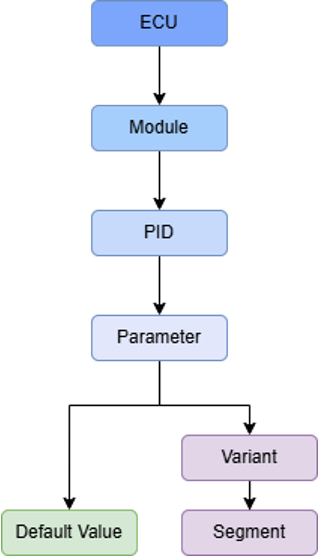
\includegraphics[height=0.4\textheight]{figures/ecu_hierarchy.png}
    \caption{Hierarchical Organization of Automotive Electronic Systems}
    \label{fig:ecu-hierarchy}
\end{figure}

This hierarchical structure is not merely organizational but reflects the actual architecture of automotive electronic systems, where software components are modularized for maintainability, reusability, and functional separation. The Common Powertrain Controller (CPC), a central \ac{ECU} in modern trucks, manages critical powertrain functions through thousands of configurable parameters organized into this hierarchical structure \cite{staron2021automotive}.

Parameters themselves have complex characteristics beyond simple values. They can be scalar values, one-dimensional arrays (curves), or multi-dimensional arrays (maps or tables). Each parameter has specific attributes defining its data type, valid range, engineering units, scale factors, and default values \cite{pretschner2007software}. For instance, an engine timing map might be represented as a two-dimensional array where engine speed and load are the independent variables, and ignition timing angle is the dependent variable. This complexity in parameter structure creates specific requirements for the database system designed to manage them.

\subsection{Parameter Variants and Customization}
\label{subsec:parameter-variants}

A fundamental challenge in automotive parameter management is supporting multiple parameter configurations for different vehicle variants, regional requirements, and operating conditions. Rather than maintaining separate complete parameter sets for each configuration, which would lead to significant redundancy, automotive systems implement a variant mechanism that allows selective overriding of parameter values based on specific conditions \cite{staron2021automotive}.

In this approach, each parameter has a default value defined in the baseline configuration. Variants are created to represent specific vehicle configurations or conditions, and segments define modified parameter values within these variants. If no segment exists for a particular parameter in an applicable variant, the default value is used. This approach minimizes redundancy by storing only the modified values rather than complete parameter sets for each configuration \cite{broy2006challenges}.

\begin{figure}[ht]
    \centering
    %\includegraphics[width=0.85\textwidth]{figures/variant_concept.png}
    \caption{Parameter Variant and Segment Concept}
    \label{fig:variant-concept}
\end{figure}

Variants are associated with code rules—boolean expressions that determine when a variant applies based on vehicle configuration codes. For example, a variant might apply only to vehicles with a specific engine type and transmission combination, or to vehicles destined for a particular market with unique regulatory requirements. The code rule evaluation process selects the appropriate variants for a specific vehicle configuration during parameter file generation \cite{staron2021autosar}.

This variant approach creates specific requirements for the database system, which must efficiently store and retrieve variant definitions and segment values while maintaining the relationships between parameters, variants, and segments. The system must also implement a parameter resolution process that correctly applies variants based on vehicle configuration codes, ensuring that the right parameter values are used for each specific vehicle.

\subsection{Release and Phase Management}
\label{subsec:release-phase-management}

Automotive software development follows a structured release process with well-defined phases representing increasing levels of maturity and stability \cite{broy2006challenges}. For parameter management, this translates into a phase-based development process where parameter configurations evolve through sequential stages before being released for production.

The typical release cycle in automotive parameter development consists of bi-annual releases (e.g., "24.1" and "24.3" for first and third quarters of 2024), with each release progressing through four sequential phases: Initial, PreTest1, PreTest2, and Final \cite{pretschner2007software}. Different \acp{ECU} may progress through these phases at different rates, requiring the parameter management system to support concurrent work on multiple phases.

\begin{figure}[ht]
    \centering
    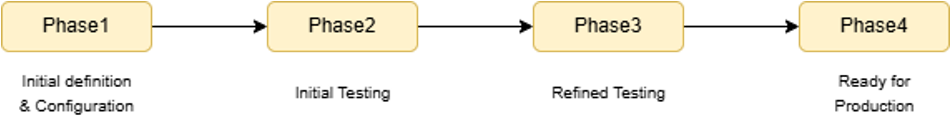
\includegraphics[width=0.85\textwidth]{figures/release_cycle.png}
    \caption{Automotive Parameter Release Cycle}
    \label{fig:release-cycle}
\end{figure}

Each phase represents a milestone in the development process with specific activities and quality gates. The Initial phase involves the creation of new parameters and initial configuration. PreTest1 and PreTest2 phases involve refinement based on testing feedback, with increasing levels of validation. The Final phase represents the completed configuration ready for production release \cite{staron2021automotive}.

When a phase transitions to the next stage, parameter configurations are copied forward, establishing a new baseline for continued development. Changes made in earlier phases should propagate to later phases unless explicitly overridden, creating a complex versioning requirement for the parameter management system \cite{pretschner2007software}. Additionally, at specific development milestones, phases may be "frozen" to create stable reference points for documentation and testing, requiring the parameter management system to enforce read-only access to frozen phases while still allowing continued development in active phases.

This phase-based release process establishes specific requirements for the database system's versioning model, which must maintain distinct parameter configurations for each phase while supporting phase transitions, change propagation, and selective freezing. The versioning approach must align with this development process rather than implementing a generic temporal model, ensuring that the system supports the actual workflows used in automotive parameter development.


\section{Database Management Systems}
\label{sec:database-management-systems}

Database management systems (DBMS) serve as the foundation for structured information storage and retrieval. They provide mechanisms for storing, organizing, and accessing data while ensuring integrity, security, and concurrent access \cite{elmasri2015fundamentals}. For the\ac{VMAP} system, selecting an appropriate database approach is critical for meeting the complex requirements of automotive parameter management.

\subsection{Relational Database Management Systems}
\label{subsec:relational-database-management-systems}

Relational Database Management Systems (RDBMS) organize data into structured tables composed of rows and columns, based on the relational model proposed by E.F. Codd in 1970 \cite{codd1970relational}. The relational model establishes a mathematical foundation for representing data as relations (tables) with well-defined operations for data manipulation. This approach has dominated database technology for decades due to its solid theoretical foundation and practical advantages for structured data management.

In relational databases, tables adhere to predefined schemas that specify the structure, data types, and constraints applicable to the data. Each table typically includes a primary key that uniquely identifies each row, while foreign keys establish relationships between tables, implementing the referential integrity that ensures consistency across related data \cite{elmasri2015fundamentals}.

A key strength of relational databases is their adherence to ACID properties (Atomicity, Consistency, Isolation, Durability), which ensure reliable transaction processing. Atomicity guarantees that transactions are treated as indivisible units that either complete entirely or have no effect. Consistency ensures that transactions maintain database integrity by transforming the database from one valid state to another. Isolation prevents interference between concurrent transactions, making them appear as if executed sequentially. Durability ensures that committed transactions persist even after system failures \cite{elmasri2015fundamentals}.

ACID compliance makes relational databases particularly suitable for automotive parameter management, where data integrity and consistency are paramount. Incorrect parameter values could potentially affect vehicle safety and performance, making the strong consistency guarantees of relational databases essential for maintaining data integrity \cite{staron2021automotive}. Additionally, the hierarchical structure of automotive parameter systems—with well-defined relationships between \acp{ECU}, modules, PIDs, and parameters—aligns naturally with the relational model's representation of structured data and relationships.

\begin{figure}[ht]
    \centering
    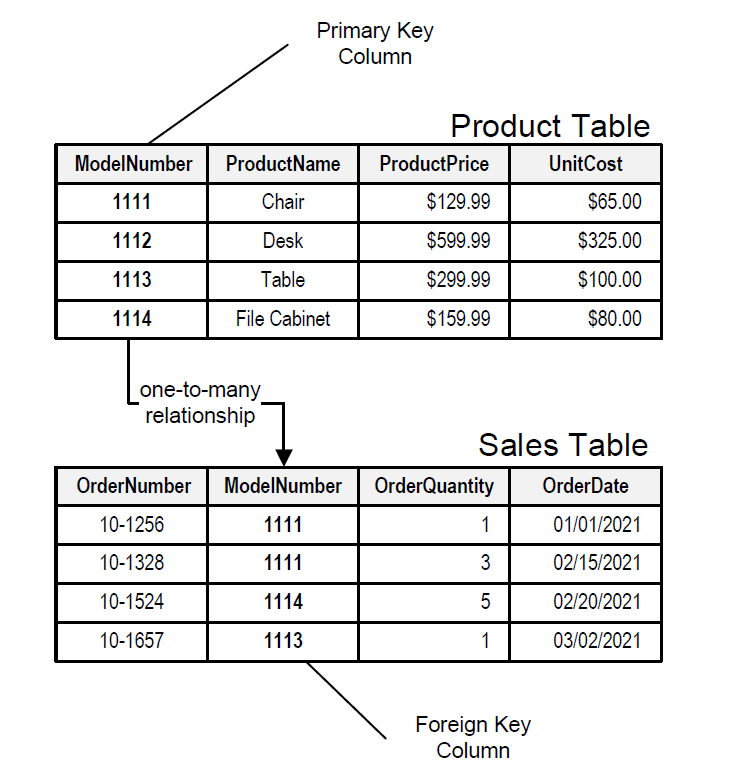
\includegraphics[width=0.85\textwidth]{figures/relational_schema.png}
    \caption{Example of a Relational Schema \cite{noah2024relational}}
    \label{fig:relational-schema}
\end{figure}

\subsection{Non-Relational Database Systems}
\label{subsec:non-relational-database-systems}

Non-relational databases, often referred to as NoSQL (Not Only SQL) databases, emerged as alternatives to the relational model, particularly for use cases involving large-scale distributed systems, unstructured data, or schema flexibility requirements. Unlike relational databases, NoSQL systems typically sacrifice some aspects of ACID compliance in favor of scalability, flexibility, and performance characteristics suited to specific application domains \cite{bhattacherjee2015principles}.

NoSQL databases can be categorized into several types based on their data models: document databases (MongoDB, CouchDB), key-value stores (Redis, DynamoDB), column-family stores (Cassandra, HBase), and graph databases (Neo4j, Amazon Neptune). Many NoSQL systems follow the BASE principle (Basically Available, Soft state, Eventually consistent) rather than ACID, prioritizing availability and partition tolerance over immediate consistency \cite{brewer2000robust}.

While NoSQL databases excel in specific domains such as high-volume web applications, real-time analytics, and social networks, they present challenges for applications requiring complex transactions, strict data integrity, or sophisticated query capabilities across related entities \cite{kleppmann2017conflict}. For automotive parameter management, these limitations make NoSQL systems generally less suitable than relational databases.

The potential for eventual consistency rather than immediate consistency in many NoSQL systems could lead to incorrect parameter configurations being used during development or testing, creating significant risks for vehicle performance and safety. Additionally, the hierarchical nature of automotive electronic systems, with well-defined relationships between entities, aligns naturally with the relational model's approach to representing structured data and relationships. The ability to enforce these relationships through foreign key constraints provides important safeguards against data inconsistency that would be more difficult to implement in many NoSQL systems.

\begin{figure}[ht]
    \centering
    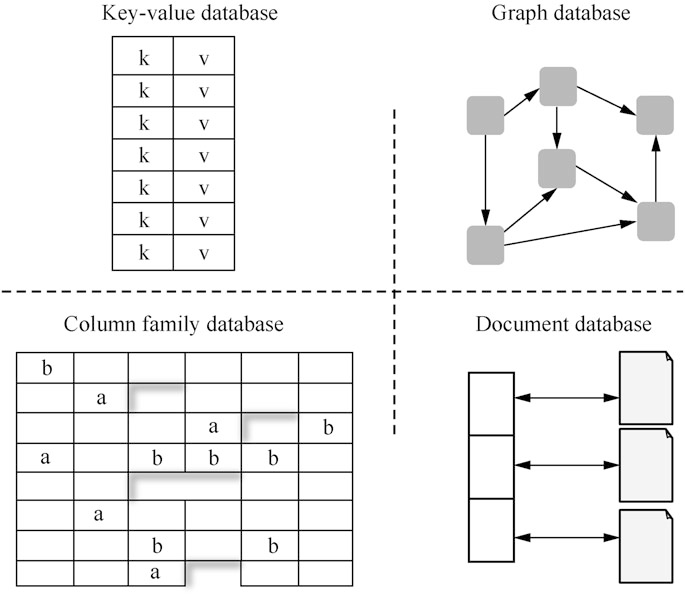
\includegraphics[width=0.85\textwidth]{figures/nosql_types.png}
    \caption{Major Types of NoSQL Databases \cite{gaussdbdatabase}}
    \label{fig:nosql-types}
\end{figure}

\section{Database Design Methodologies}
\label{sec:database-design-methodologies}

Database design methodologies provide structured approaches to creating efficient, reliable database systems. These methodologies help translate real-world information needs into technical implementations that can store and manage data effectively. This section explores fundamental approaches that form the theoretical foundation for database design, presented in a sequence that follows the natural progression from user requirements to technical implementation.

\subsection{Use Case Modeling}
\label{subsec:use-case-modeling}

Before designing a database structure, it is essential to understand how users will interact with the system. Use case modeling provides a technique for capturing user requirements by identifying who will use the system (actors) and what they need to accomplish (use cases). Developed by Ivar Jacobson, use case modeling has become a cornerstone of requirements analysis in system development \cite{jacobson2004use}.

A use case represents a specific goal that an actor wishes to achieve using the system. Actors can be human users with different roles (such as administrators or regular users) or external systems that interact with the database. The collection of all use cases defines the system's functional boundaries—what it must do to satisfy user needs \cite{jacobson2004use}.

Use case diagrams provide a visual representation of these relationships, showing actors as stick figures and use cases as ovals, with lines connecting actors to their associated use cases. This visual format makes the system's purpose accessible to non-technical stakeholders, facilitating communication between developers and users. As noted by Jacobson, "Use cases bridge the gap between the users' and the developers' views of the system" \cite{jacobson2004use}.

For automotive parameter management systems, use case modeling helps identify the different ways in which engineers, documentation specialists, administrators, and other stakeholders need to interact with parameter data. These use cases then inform the database design, ensuring that the resulting structure effectively supports all required operations.


\begin{figure}[ht]
    \centering
    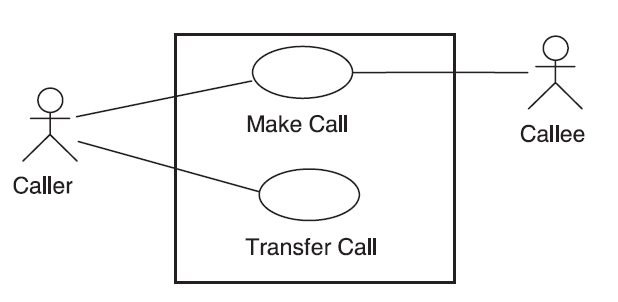
\includegraphics[width=0.85\textwidth]{figures/use_case_diagram.png}
    \caption{Use Case Diagram of switching system \cite{jacobson2004use}}
    \label{fig:use-case-diagram}
\end{figure}

\subsection{Entity-Relationship Modeling}
\label{subsec:entity-relationship-modeling}

After understanding user requirements through use cases, the next step is to model the data itself. Entity-Relationship (ER) modeling provides a conceptual framework for representing the data structure needed to support the identified use cases. Introduced by Peter Chen in 1976, ER modeling has become the most widely used approach for conceptual database design \cite{chen1976entity}.

ER modeling identifies three main components:

Entities represent the objects or concepts about which information needs to be stored. In an automotive context, these might include vehicles, electronic control units (ECUs), parameters, and users. Entities are represented as rectangles in ER diagrams.

Attributes describe the specific properties or characteristics of each entity. For example, a parameter entity might have attributes like name, value, unit, and description. Attributes are shown as ovals connected to their entity.

Relationships describe the associations between entities. For instance, "ECUs contain parameters" expresses a relationship between \ac{ECU} and parameter entities. Relationships are shown as diamonds connecting the related entities, with cardinality notations indicating how many instances of each entity can participate in the relationship \cite{elmasri2015fundamentals}.

ER modeling is particularly valuable for complex domains like automotive systems because it provides a visual representation that stakeholders can understand while being precise enough to guide database implementation. Chen explains that "the entity-relationship model adopts the more natural view that the real world consists of entities and relationships" \cite{chen1976entity}, making it an intuitive approach for modeling real-world systems.

\begin{figure}[ht]
    \centering
    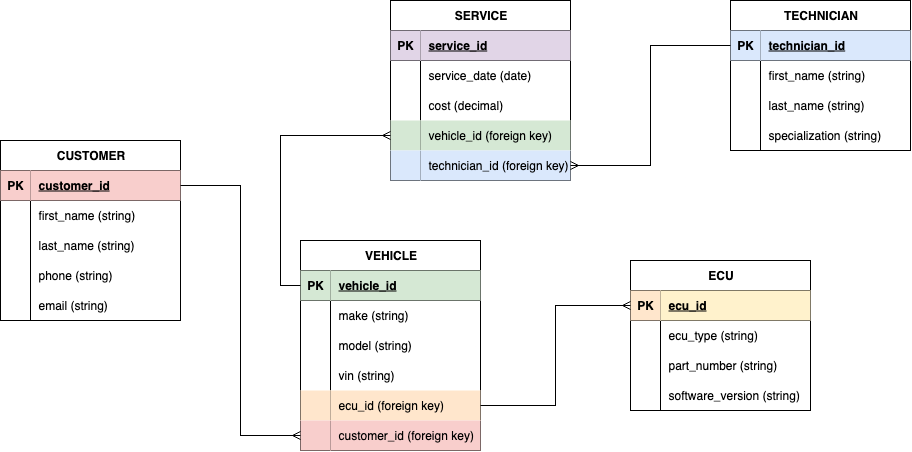
\includegraphics[width=0.85\textwidth]{figures/er_diagram.png}
    \caption{Entity-Relationship Diagram for Core\ac{VMAP} Entities \cite{RelationalData}}
    \label{fig:er-diagram}
\end{figure}

\subsection{Database Normalization}
\label{subsec:database-normalization}

Once the conceptual model is established through ER modeling, database normalization helps refine this model into an efficient, consistent structure. Normalization is a systematic process developed by E.F. Codd that organizes data to minimize redundancy and avoid update anomalies \cite{codd1970relational}.

Normalization proceeds through several "normal forms," each addressing specific types of data inconsistencies:

First Normal Form (1NF) requires that each cell in a table contains only a single value, not a list of values. For example, storing multiple phone numbers in a single field would violate 1NF. This ensures that data is atomic (indivisible) and can be manipulated consistently.

Second Normal Form (2NF) builds on 1NF by requiring that all non-key attributes depend on the entire primary key, not just part of it. This prevents situations where changing one piece of data requires multiple updates in different places.

Third Normal Form (3NF) further refines the structure by requiring that non-key attributes depend only on the primary key, not on other non-key attributes. This eliminates transitive dependencies that can lead to update anomalies \cite{elmasri2015fundamentals}.

For most practical applications, achieving 3NF provides a good balance between data integrity and system performance. As explained by Date, "Third normal form is considered adequate for most practical purposes; further normalization is usually performed only when necessary" \cite{date2011sql}.

In automotive parameter management, normalization helps organize complex data about \acp{ECU}, modules, and parameters into a structure that maintains consistency while supporting efficient access. For example, normalizing parameter data ensures that when a parameter value changes, that change only needs to be recorded in one place, eliminating the risk of inconsistent values across the database.

\subsection{Role-Based Access Control Models}
\label{subsec:role-based-access-control}

Database systems often contain sensitive information that should not be accessible to all users. Role-Based Access Control (RBAC) provides a structured approach to managing permissions within a database system. Introduced by David Ferraiolo and Richard Kuhn in the 1990s, RBAC has become the predominant model for access control in enterprise systems due to its balance of security and administrative simplicity \cite{sandhu1998role}.

The core concept of RBAC is that permissions are associated with roles, and users are assigned to appropriate roles rather than being granted permissions directly. A role represents a specific function within an organization, such as ``administrator,'' ``engineer,'' or ``analyst.'' Each role is granted a set of permissions that allow users assigned to that role to perform specific operations on database objects like reading, creating, updating, or deleting records \cite{ferraiolo2011policy}.

This structure provides several important advantages over direct permission assignment. First, it simplifies administration by allowing permissions to be managed at the role level rather than the individual user level. When a new user joins the organization, they can simply be assigned to the appropriate roles rather than requiring configuration of individual permissions. Second, it improves security by implementing the principle of least privilege, ensuring that users have only the permissions necessary for their specific responsibilities which reduces the risk of unauthorized access or accidental data modifications \cite{sandhu1998role}.

The theoretical foundation of RBAC includes several key components: users (individuals who need access to the system), roles (collections of permissions that correspond to job functions), permissions (defined operations on specific resources), and sessions (temporary bindings between users and their assigned roles). These components provide a flexible framework for implementing access control policies tailored to specific organizational needs while maintaining a clear separation between users and permissions through the role abstraction \cite{sandhu1997arbac97}.


\subsection{Version Control for Databases}
\label{subsec:database-versioning}

Version control for databases addresses the challenge of tracking changes to data structures and content over time. Unlike traditional file-based version control systems designed for source code, database versioning must maintain complex relationships between entities while preserving historical states and supporting evolution through distinct development stages \cite{bhattacherjee2015principles}.

Several approaches have emerged for implementing version control in database systems. The snapshot approach captures complete database states at specific points in time, providing simple retrieval of historical states but potentially consuming significant storage resources. The change-based approach records only modifications to database content, reducing storage requirements but requiring reconstruction of historical states through the application of change records \cite{bhattacherjee2015principles}.

The temporal approach extends traditional database structures with time dimensions, enabling direct querying of historical states through time-based predicates. This approach typically introduces valid time (when facts are true in the real world) and transaction time (when facts are recorded in the database) dimensions, allowing sophisticated historical analysis but adding complexity to schema design and query formulation \cite{snodgrass1999developing}.

Phase-based versioning represents a domain-specific approach that aligns database versioning with development phases rather than continuous time. This approach explicitly models development stages as first-class entities in the database schema, associating data with specific phases rather than temporal timestamps. According to Bhattacherjee et al., "Domain-specific versioning approaches often provide better performance and usability than generic temporal database techniques when tailored to specific application requirements" \cite{bhattacherjee2015principles}.


\subsection{Temporal Database Concepts}
\label{subsec}

Many applications, including automotive parameter management, need to track how data changes over time. Temporal database concepts address these requirements by providing mechanisms for managing time-varying data. Unlike traditional databases that store only the current state, temporal databases maintain historical states and support queries based on time dimensions \cite{snodgrass1999developing}.

Temporal databases typically support two key time dimensions. Valid time represents when facts are true in the modeled reality—for example, when a particular parameter configuration becomes active in a vehicle. Transaction time represents when facts are recorded in the database—for example, when a parameter value was updated in the system. Databases that support both dimensions are known as bi-temporal databases \cite{kulkarni2012temporal}.

Temporal database implementations often use specialized table structures called temporal tables. These tables extend traditional table structures with additional timestamp columns that define the time periods during which each record is valid. For example, a temporal parameter table might include ValidFrom and ValidTo columns that define when each parameter value is applicable, allowing the database to maintain a complete history of parameter changes \cite{salzberg1999comparison}.

Kulkarni and Michels explain that "temporal tables provide a systematic way to track and query historical data without requiring application-level version management" \cite{kulkarni2012temporal}. This capability is particularly valuable in regulated industries like automotive development, where traceability and auditability of parameter changes are essential for compliance and quality assurance.

In automotive parameter management, temporal database concepts can support critical requirements such as tracking parameter evolution throughout the development lifecycle, maintaining historical records for diagnostic and compliance purposes, and enabling historical analysis to understand how parameter configurations have evolved over time. These capabilities form an important theoretical foundation for designing systems that manage time-sensitive data in complex domains.

\begin{figure}[ht]
    \centering
    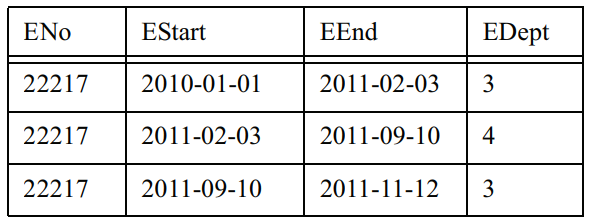
\includegraphics[width=0.85\textwidth]{figures/temporal_database.png}
    \caption{Temporal Database Example \cite{kulkarni2012temporal}}
    \label{fig:temporal-database}
\end{figure}

\subsection{Strategic Denormalization}
\label{subsec:strategic-denormalization}

While normalization provides a theoretical foundation for database integrity, practical database design often requires balancing normalization principles with performance considerations. Strategic denormalization involves deliberately introducing controlled redundancy to improve performance for specific operations \cite{bhattacherjee2015principles}.

Consider a fully normalized database where information about parameters, their modules, and their \acp{ECU} is stored in separate tables. To retrieve a parameter with its associated module and \ac{ECU} information would require joining all three tables—an operation that becomes increasingly expensive as the database grows. In cases where this retrieval happens frequently, storing the module and \ac{ECU} names directly in the parameter table (introducing controlled redundancy) could significantly improve performance \cite{schwartz2012high}.

Molinaro emphasizes that "denormalization is not about abandoning normalization principles, but about making strategic exceptions for performance reasons" \cite{molinaro2005sql}. These exceptions should be carefully documented and justified based on specific performance requirements.

For automotive systems, where both data integrity and query performance are critical, finding the right balance between normalization and strategic denormalization is essential. This balance ensures that parameter data maintains consistency while providing the performance needed for engineering workflows.

\subsection{Conceptual, Logical, and Physical Design Levels}
\label{subsec:design-levels}

Database design typically proceeds through three levels of abstraction, allowing designers to manage complexity by focusing on different aspects at each stage:

Conceptual design focuses on what data needs to be stored, without concern for implementation details. The ER model created at this stage captures entities, attributes, and relationships from a business perspective, providing a foundation that both technical and non-technical stakeholders can understand \cite{elmasri2015fundamentals}.

Logical design transforms the conceptual model into structures specific to the chosen database model (typically relational), defining tables, columns, keys, and relationships. This stage applies normalization principles to refine the structure, independent of any specific database system \cite{elmasri2015fundamentals}.

Physical design addresses how the logical design will be implemented in a specific database management system, considering factors like storage structures, indexing strategies, and access methods. This stage optimizes the design for performance based on anticipated usage patterns \cite{obe2017postgresql}.

Moving through these levels allows database designers to progressively refine the database structure, addressing different concerns at each stage. As Elmasri and Navathe observe, "The separation of conceptual, logical, and physical design allows database designers to focus on the appropriate level of abstraction at each stage" \cite{elmasri2015fundamentals}.

For automotive parameter management, this layered approach helps manage the complexity of the domain, ensuring that the resulting database effectively supports both the business requirements (storing and managing parameter configurations) and the technical requirements (performance, scalability, and maintainability).
    \cleardoublepage
    \chapter{State of the Art}
\label{chap:state-of-art}

This chapter examines the current state of the art in database version control systems and automotive parameter management. It begins by analyzing existing approaches to software configuration management in the automotive industry, followed by an evaluation of database versioning techniques and their applicability to parameter management systems. The chapter also explores role-based access control models and integration strategies for enterprise systems, establishing the theoretical foundation for the VMAP system design.

\section{Parameter Management in Automotive Software Development}
\label{sec:parameter-management}

The complexity of automotive software has grown exponentially in recent decades, with modern vehicles containing up to 100 million lines of code distributed across dozens of electronic control units (ECUs) \cite{pretschner2007software}. This growth has significantly increased the importance and complexity of parameter management in automotive development.

\subsection{Evolution of Automotive Parameter Management}
\label{subsec:evolution-parameter-management}

Parameter management in automotive systems has evolved from simple calibration tables to sophisticated configuration frameworks managing thousands of parameters across multiple vehicle variants. Broy \cite{broy2006challenges} describes the fundamental challenges in automotive software engineering, highlighting that software complexity is driven by the need to address multiple variants, market requirements, and technical functions. The parameter configuration problem is specifically identified as one of the key challenges in this domain.

Early approaches to parameter management relied on specialized tools provided by ECU suppliers, which typically stored parameters in proprietary formats with limited version control capabilities. Pretschner et al. \cite{pretschner2007software} note that these tools evolved from simple memory editors to more sophisticated calibration environments, but remained focused on individual ECUs rather than system-wide parameter management.

Staron \cite{staron2021automotive} describes how AUTOSAR (Automotive Open System Architecture) has contributed to more structured parameter management by defining standard interfaces and component models that separate parameters from implementation. However, the practical implementation of these standards varies across organizations and ECU suppliers, creating integration challenges for comprehensive parameter management.

\subsection{Challenges in Automotive Parameter Management}
\label{subsec:challenges-parameter-management}

The management of parameters in automotive software development presents specific challenges that distinguish it from general software configuration management. Pretschner et al. \cite{pretschner2007software} identify several key challenges related to variability management in automotive software, including the need to maintain multiple parameter configurations for different vehicle variants, markets, and operating conditions.

Broy \cite{broy2006challenges} emphasizes the challenge of managing interdependencies between parameters, noting that changes to one parameter often require coordinated changes to related parameters to maintain system consistency. This creates a need for sophisticated dependency tracking mechanisms that go beyond traditional version control systems.

Another significant challenge relates to validation requirements for parameter changes. Unlike source code, which can be validated through compilation and static analysis, parameters require functional testing to verify their correctness. Pretschner et al. \cite{pretschner2007software} describe how this validation often involves specialized hardware-in-the-loop or vehicle-level testing, creating a significant gap between parameter modification and validation.

Kiencke and Nielsen \cite{kiencke2000automotive} discuss the specific challenges related to powertrain control parameters, noting the complex interactions between engine control parameters and their effects on vehicle performance, emissions, and fuel economy. These interactions create a need for sophisticated parameter testing and validation processes beyond simple version control.

\subsection{Current Approaches and Tools}
\label{subsec:current-approaches-tools}

Current parameter management solutions in the automotive industry span a spectrum from general-purpose tools to specialized automotive calibration systems. 

Staron \cite{staron2021automotive} discusses how AUTOSAR tools provide standardized interfaces for parameter management in modern automotive systems, but notes that these tools focus primarily on the technical aspects of parameter definition rather than the organizational processes of parameter development and validation through multiple development phases.

Broy \cite{broy2006challenges} identifies the challenges of integrating parameter management into broader software development processes, noting that many organizations maintain separate workflows for software development and parameter calibration. This separation creates coordination challenges, particularly when parameter changes affect multiple software components or require software modifications.

Pretschner et al. \cite{pretschner2007software} discuss how model-based development approaches are increasingly used in automotive development, with parameters linked to model elements to provide traceability and support automated validation. However, they note that the integration between parameter management tools and modeling environments remains incomplete in many organizations.

For database-oriented approaches to parameter management, Bhattacherjee et al. \cite{bhattacherjee2015principles} provide a theoretical foundation by examining the principles of dataset versioning. They describe the fundamental trade-offs between storage efficiency and reconstruction performance, which are particularly relevant for systems that must maintain multiple parameter configurations across different development phases.

\section{Database Version Control Systems}
\label{sec:database-version-control}

Version control for database content presents distinct challenges compared to traditional source code version control. While source code version control focuses on tracking changes to text files, database version control must address structured data with complex relationships and constraints \cite{bhattacherjee2015principles}. This section examines current approaches to database version control and their applicability to automotive parameter management.

\subsection{Traditional Database Versioning Approaches}
\label{subsec:traditional-database-versioning}

Traditional approaches to database versioning fall into several categories, each addressing different aspects of the versioning challenge. Schema evolution tools focus on tracking and managing changes to database structure through migration scripts or schema manipulation languages. Curino et al. \cite{curino2009automating} describe an approach for automating database schema evolution in information system upgrades, focusing on maintaining data integrity during schema transitions.

Bhattacherjee et al. \cite{bhattacherjee2015principles} provide a comprehensive analysis of dataset versioning approaches, identifying a fundamental trade-off between storage and recreation costs. They categorize versioning strategies into several approaches:

1. Version-first approaches maintain complete snapshots of datasets at specific version points, providing simple retrieval of historical states but requiring substantial storage space.

2. Delta-based approaches store only the changes between versions, reducing storage requirements but increasing the computational cost of reconstructing historical states.

3. Hybrid approaches combine elements of both strategies, typically storing periodic full snapshots with incremental deltas between snapshots.

The authors note that the optimal strategy depends on specific usage patterns, particularly the ratio between storage costs and the frequency and complexity of historical data access operations.

Mueller and Müller \cite{mueller2018conception} describe a practical implementation of database versioning between research institutes, highlighting the challenges of maintaining consistency across systems with different update cycles. Their approach uses a combination of schema versioning and data synchronization mechanisms to maintain consistency while supporting independent evolution.

\subsection{Temporal Database Approaches}
\label{subsec:temporal-database-approaches}

Temporal database approaches provide a theoretical foundation for managing time-varying data in database systems. Kulkarni and Michels \cite{kulkarni2012temporal} describe the temporal features introduced in SQL:2011, which formalized support for period data types and temporal tables in the SQL standard. These features enable tracking of both valid time (business time) and transaction time (system time) dimensions, supporting bi-temporal data management.

The valid time dimension represents when facts are true in the modeled reality, independent of when they are recorded in the database. This dimension supports business-oriented temporal queries such as "What was the value of this parameter in a specific phase?" or "When did this parameter change from value A to value B?" \cite{bohlen2018database}. The transaction time dimension represents when facts are recorded in the database, supporting auditability through questions like "Who changed this parameter, and when did they change it?" \cite{kulkarni2012temporal}.

Bi-temporal databases combine both dimensions, providing a comprehensive framework for tracking both when changes occurred in the system and when they became effective in the real world \cite{bohlen2018database}. This approach is particularly valuable for regulated industries like automotive development, where both historical accuracy and change auditability are essential for compliance and quality assurance.

Snodgrass \cite{snodgrass1999developing} provides a comprehensive guide to developing time-oriented database applications in SQL, describing practical techniques for implementing temporal functionality in relational database systems. The author presents various approaches to tracking historical data, including transaction-time tables, valid-time tables, and bi-temporal tables, with practical implementation guidance for each approach.

Biriukov \cite{biriukov2018implementation} examines practical implementation aspects of bi-temporal databases, highlighting the challenges of schema design, query formulation, and performance optimization. The author notes that domain-specific temporal approaches often provide more practical solutions than generic bi-temporal frameworks, particularly for applications with specialized temporal requirements.

\subsection{Version Control for Parameter Management}
\label{subsec:version-control-parameter-management}

Version control for automotive parameter management presents specific requirements that differ from general database versioning needs. Drawing from the literature, several key requirements can be identified:

Broy \cite{broy2006challenges} discusses the need for version control approaches that align with automotive development processes, which typically follow a structured progression through predefined development phases. Unlike source code versioning, which often follows continuous development with arbitrary version points, parameter versioning must support specific phase-based workflows.

Bhattacherjee et al. \cite{bhattacherjee2015principles} examine the trade-offs between different versioning strategies, which are particularly relevant for parameter management systems that must maintain multiple configurations across different development phases. The authors' analysis of storage versus reconstruction costs provides a theoretical foundation for designing efficient parameter versioning systems.

Snodgrass \cite{snodgrass1999developing} describes techniques for tracking valid-time information in database systems, which aligns with the need to maintain parameter configurations that are valid for specific development phases or vehicle configurations. However, the author's focus on general temporal database approaches does not address the specific requirements of phase-based development.

Bhattacherjee et al. \cite{bhattacherjee2015principles} note that domain-specific versioning systems often provide more effective solutions than generic versioning frameworks, particularly for domains with structured development processes and complex entity relationships. This observation supports the development of specialized versioning approaches tailored to automotive parameter management rather than adopting generic temporal database techniques.

\section{Role-Based Access Control in Enterprise Systems}
\label{sec:role-based-access-control}

Role-Based Access Control (RBAC) has become a dominant paradigm for managing access rights in enterprise systems, providing a structured approach to security management that aligns with organizational responsibilities \cite{sandhu1998role}. For automotive parameter management, where different user roles have distinct responsibilities and access requirements, RBAC provides a foundation for implementing appropriate security controls.

\subsection{RBAC Model and Extensions}
\label{subsec:rbac-model-extensions}

The core RBAC model, as defined by Sandhu et al. \cite{sandhu1998role}, consists of users, roles, permissions, and sessions. Users are assigned to roles that correspond to job functions, and roles are granted permissions that authorize specific operations on protected resources. This indirect association between users and permissions through roles simplifies security administration while maintaining the principle of least privilege.

Several extensions to the basic RBAC model have been developed to address more complex security requirements. Sandhu et al. \cite{sandhu1998role} describe hierarchical RBAC, which introduces role hierarchies that enable permission inheritance between roles, supporting organizational structures with senior roles inheriting permissions from junior roles.

Sandhu and Bhamidipati \cite{sandhu1997arbac97} present administrative RBAC (ARBAC), which addresses the management of the RBAC system itself, defining who can assign users to roles and modify role permissions. This extension is particularly relevant for enterprise systems where role and permission management is distributed across different administrative domains.

Ferraiolo et al. \cite{ferraiolo2011policy} describe policy-enhanced RBAC, which combines role-based permissions with attribute-based policies to provide context-sensitive access control. This hybrid approach is particularly valuable for systems where access decisions depend on both user roles and context-specific factors such as time, location, or resource attributes.

\subsection{RBAC in Database Systems}
\label{subsec:rbac-database-systems}

Modern database management systems provide varying levels of support for RBAC principles. Elmasri and Navathe \cite{elmasri2015fundamentals} describe the evolution of database security mechanisms from simple user-based privileges to more sophisticated role-based models. Most enterprise database systems now include native support for roles, user-role assignments, and permission management through SQL statements like GRANT and REVOKE.

Obe and Hsu \cite{obe2017postgresql} detail PostgreSQL's implementation of RBAC concepts, including role hierarchies through role inheritance, permission management through fine-grained privileges, and row-level security policies for content-based access control. These capabilities provide a foundation for implementing domain-specific access control models on top of the database system's native security features.

However, database-level RBAC implementations typically focus on controlling access to database objects like tables, views, and functions, rather than providing application-level access control that considers domain-specific entities and operations. For complex applications like automotive parameter management, database-level RBAC must be complemented with application-level access control logic that maps domain-specific concepts to database operations \cite{ferraiolo2011policy}.

\subsection{Access Control for Parameter Management}
\label{subsec:access-control-parameter-management}

Access control for automotive parameter management presents specific requirements that extend beyond basic RBAC models. Drawing from the literature, several key access control requirements can be identified:

Sandhu et al. \cite{sandhu1998role} provide the theoretical foundation for role-based access control, which aligns with the organizational structure of automotive development teams. Different roles such as parameter engineers, module developers, and system integrators require different access rights to parameter data.

Ferraiolo et al. \cite{ferraiolo2011policy} describe policy-enhanced RBAC, which combines role-based permissions with attribute-based policies. This hybrid approach is particularly relevant for parameter management, where access rights may depend on both user roles and attributes of the parameters being accessed, such as their development phase or module assignment.

Hu et al. \cite{hu2015implementing} discuss practical aspects of implementing and managing policy rules in attribute-based access control, providing insights into the challenges of combining role-based and attribute-based approaches. Their work highlights the importance of balancing security requirements with usability considerations, which is particularly relevant for parameter management systems used by diverse stakeholder groups.

Sandhu and Bhamidipati \cite{sandhu1997arbac97} address the administrative aspects of RBAC, which are important for parameter management systems where access control administration may be distributed across different organizational units. Their ARBAC97 model provides a framework for delegating administrative responsibilities while maintaining central governance.

\section{Database Integration with Enterprise Systems}
\label{sec:database-integration}

Integration between database systems and enterprise applications presents significant challenges in automotive development environments, where parameter management must interact with numerous other systems across the development lifecycle. Effective integration strategies must address both technical interoperability and semantic consistency while maintaining performance and security \cite{hohpe2002enterprise}.

\subsection{Enterprise Integration Patterns}
\label{subsec:enterprise-integration-patterns}

Enterprise integration patterns, as documented by Hohpe and Woolf \cite{hohpe2002enterprise}, provide a catalog of solutions for common integration challenges. These patterns address various aspects of system integration, including messaging styles, messaging channels, message construction, and message transformation.

For database-centric applications like parameter management systems, several integration patterns are particularly relevant. Fowler \cite{fowler2003patterns} describes the Repository pattern, which provides a structured approach to data access, abstracting the database implementation details behind a domain-focused interface. This abstraction simplifies integration by providing a stable API for other systems to interact with the parameter repository.

Fowler \cite{fowler2003patterns} also documents the Data Transfer Object (DTO) pattern, which addresses the challenge of transferring data between systems with different data models. By defining specialized objects for inter-system communication, this pattern enables consistent data exchange while isolating each system's internal representation.

The Canonical Data Model pattern, as described by Hohpe and Woolf \cite{hohpe2002enterprise}, establishes a common data representation across multiple systems, simplifying data transformation and ensuring consistent interpretation. This pattern is particularly valuable for parameter management, where the same parameter concepts may be represented differently in various systems across the development lifecycle.

\subsection{Database Synchronization Approaches}
\label{subsec:database-synchronization}

Database synchronization presents specific challenges when integrating parameter management systems with other enterprise data sources. Mueller and Müller \cite{mueller2018conception} describe approaches to database versioning and synchronization between research institutes, highlighting the challenges of maintaining consistency across systems with different update cycles.

Bhattacherjee et al. \cite{bhattacherjee2015principles} discuss the principles of dataset versioning, which are relevant for synchronization between parameter management systems and other enterprise databases. Their analysis of the trade-offs between storage and recreation costs provides insights into designing efficient synchronization mechanisms that minimize both data transfer volumes and processing overhead.

Seenivasan and Vaithianathan \cite{seenivasan2023real} examine change data capture (CDC) techniques, which enable incremental synchronization by identifying and propagating only changed data between systems. These techniques reduce synchronization overhead compared to full dataset transfers but require reliable change detection mechanisms and careful handling of interdependent changes.

Kleppmann and Beresford \cite{kleppmann2017conflict} address the challenges of conflict resolution in distributed data systems, which are relevant for parameter management systems that must synchronize with multiple enterprise data sources. Their work on conflict-free replicated data types provides theoretical foundations for designing synchronization mechanisms that maintain consistency across distributed systems.

\section{Summary and Research Gaps}
\label{sec:summary-gaps}

The review of existing literature reveals several research gaps in the domain of database systems for automotive parameter management:

Current database versioning approaches, as described by Bhattacherjee et al. \cite{bhattacherjee2015principles} and Snodgrass \cite{snodgrass1999developing}, provide general frameworks for managing time-varying data but do not specifically address the phase-based development processes common in automotive parameter management. There is a need for specialized versioning approaches that align directly with automotive development workflows while providing the traceability and auditability required for regulatory compliance.

The RBAC models described by Sandhu et al. \cite{sandhu1998role} and Ferraiolo et al. \cite{ferraiolo2011policy} provide a foundation for access control but require extensions to address the specific requirements of parameter management, where access rights depend on both organizational roles and parameter-specific attributes such as module assignment and development phase.

Integration approaches documented by Hohpe and Woolf \cite{hohpe2002enterprise} and Mueller and Müller \cite{mueller2018conception} provide general patterns for system integration but do not specifically address the challenges of integrating parameter management systems with automotive-specific enterprise systems such as parameter definition databases and vehicle configuration databases.

These research gaps highlight the need for domain-specific solutions that combine insights from database version control, access control models, and enterprise integration patterns with specialized knowledge of automotive development processes. The VMAP system addresses these gaps by developing a database architecture tailored to the specific requirements of automotive parameter management, as will be detailed in subsequent chapters.
    \cleardoublepage
    \chapter{Methodology and Concept Development}
\label{chap:methodology}

This chapter presents the systematic approach taken in designing the Variant Management and Parametrization (VMAP) system. The methodology follows established software engineering principles to address the complex requirements of automotive parameter management. Beginning with a requirements analysis, the chapter proceeds to detail the conceptual architecture design, data model, validation mechanisms, and integration approaches developed to ensure system robustness and compatibility with existing enterprise infrastructure.

\section{Requirements Analysis}
\label{sec:requirements-analysis}

The foundation of the VMAP system design was a comprehensive requirements analysis combining stakeholder interviews, legacy system analysis, and industry best practice evaluation. This multi-faceted approach ensured the system would address actual user needs while overcoming limitations of existing approaches \cite{sommerville2011software}.

\subsection{Functional Requirements}
\label{subsec:functional-requirements}

The primary functional requirements derived from VMAP's fundamental purpose: replacing Excel-based parameter management with a centralized database solution. The system must support hierarchical organization of parameters within Electronic Control Units (ECUs), Modules, and Parameter IDs (PIDs), reflecting the domain-specific structure of automotive electronic systems \cite{staron2021automotive}. 

Users must be able to create variants for parameters with specific code rules determining their applicability, and define segments representing modified parameter values. If no segment exists, the system defaults to Parameter Definition Database values—an approach allowing efficient storage by tracking only modifications rather than duplicating unchanged parameters \cite{bhattacherjee2015principles}.

The system must track parameter values across four distinct release phases (Phase1, Phase2, Phase3, and Phase4), with changes in earlier phases propagating to later phases unless explicitly overridden. This phase-based approach represents a domain-specific adaptation particularly suited to automotive software development cycles \cite{broy2006challenges}.

All modifications require comprehensive logging with user information, timestamp, and detailed change data, supporting regulatory compliance and enabling parameter evolution tracking. The system must also provide functionality to create parameter configuration snapshots at specific points, particularly at phase transitions, for documentation purposes—an essential capability for quality assurance and regulatory compliance \cite{staron2021automotive}.

\subsection{User Role Requirements}
\label{subsec:user-role-requirements}

Analysis identified four distinct user roles with specific access requirements. Module developers require write access to parameters within their assigned modules, with the ability to create and modify variants and segments. Documentation specialists need access to frozen data for documentation, comparison capabilities between phases, and comprehensive change history access. System administrators require comprehensive control over user management, release phases, and special operations like variant deletion and phase freezing. Finally, read-only users need view access to all parameter data with parameter file generation capabilities but no modification rights.

These roles were defined based on the principle of least privilege \cite{sandhu1998role}, ensuring users have access only to functionality required for their specific responsibilities. This enhances system security while simplifying the user experience by presenting only relevant options. The hybrid role-permission model selected combines a primary role defining core permissions with additional permissions granted on a per-user basis, providing flexibility for special cases while maintaining a clear role structure.

\begin{figure}[h]
    \centering
    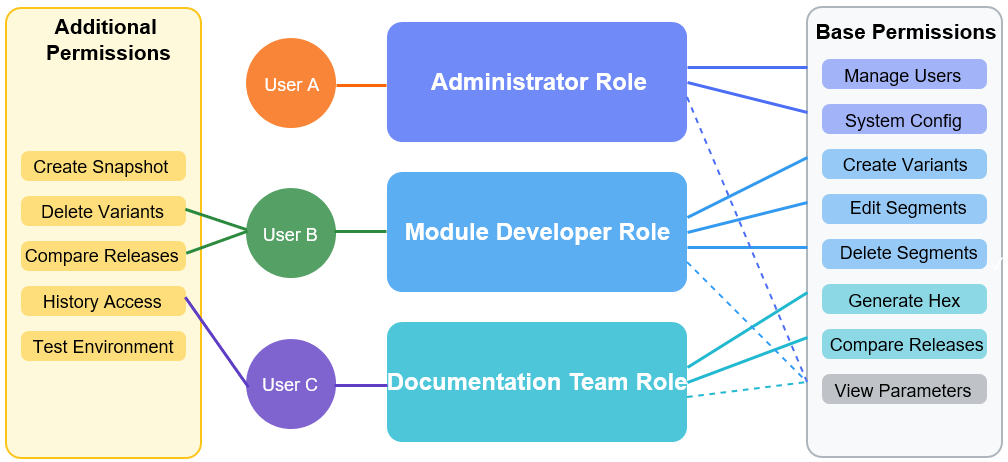
\includegraphics[width=0.95\textwidth]{figures/hybrid_role_permission_model.png}
    \caption{Hybrid Role-Permission Model}
    \label{fig:hybrid-role-model}
\end{figure}

Figure \ref{fig:hybrid-role-model} illustrates the hybrid role-permission approach that balances structured role assignments with flexible permission customization. This model supports both organizational clarity and individual access requirements.

\subsection{Data Management Requirements}
\label{subsec:data-management-requirements}

The system must maintain distinct parameter versions across different release phases, allowing simultaneous work on multiple phases while enabling access to parameter values from any development lifecycle point. Data integrity requires maintaining referential integrity across all related entities, particularly ensuring variants and segments associate with valid parameters \cite{elmasri2015fundamentals}.

Multi-dimensional parameter support is essential for complex automotive parameters such as mapping tables. Operations modifying multiple related entities must function as atomic transactions to maintain data consistency—particularly important for phase transitions where numerous parameters, variants, and segments may change simultaneously \cite{bhattacherjee2015principles}.

Query performance is critical, with efficient parameter data querying across dimensions including ECU, module, PID, release phase, and parameter name. These requirements influenced schema design decisions regarding normalization and indexing strategies to optimize common query patterns.

\subsection{Integration Requirements}
\label{subsec:integration-requirements}

VMAP must integrate with two external enterprise systems: the Parameter Definition Database (PDD) providing base ECU, module, PID, and parameter definitions; and the Vehicle Database supporting parameter file generation and variant code rule validation. The database must store necessary vehicle configuration data and maintain relationships between vehicle codes and variants, supporting practical application of parameter variants in vehicle-specific configurations \cite{staron2021automotive}.

These requirements follow enterprise integration patterns focusing on reliable data exchange, appropriate error handling, and minimal impact on existing systems \cite{hohpe2002enterprise}. The database implements these through specialized structures mapping between VMAP and external entities, tracking synchronization operations, and storing imported data with appropriate relationships to internally generated content.

\section{System Architecture Design}
\label{sec:system-architecture-design}

Based on the requirements analysis, a comprehensive system architecture was designed following a layered pattern with clear separation of concerns, enhancing maintainability while allowing independent component evolution \cite{fowler2003patterns}.

\subsection{Entity-Relationship Model}
\label{subsec:entity-relationship-model}

The entity-relationship (ER) model forms the foundation of the database design, capturing complex relationships between system entities. User management entities include Users, Roles, Permissions, and their relationships, implementing the hybrid role-permission model. Release management entities encompass Releases, Release Phases, and ECU Phase mappings, providing the foundation for version control. Parameter structure entities include ECUs, Modules, PIDs, Parameters, and Parameter Dimensions, representing the hierarchical organization of vehicle electronic systems \cite{staron2021automotive}.

\begin{figure}[htbp]
    \centering
    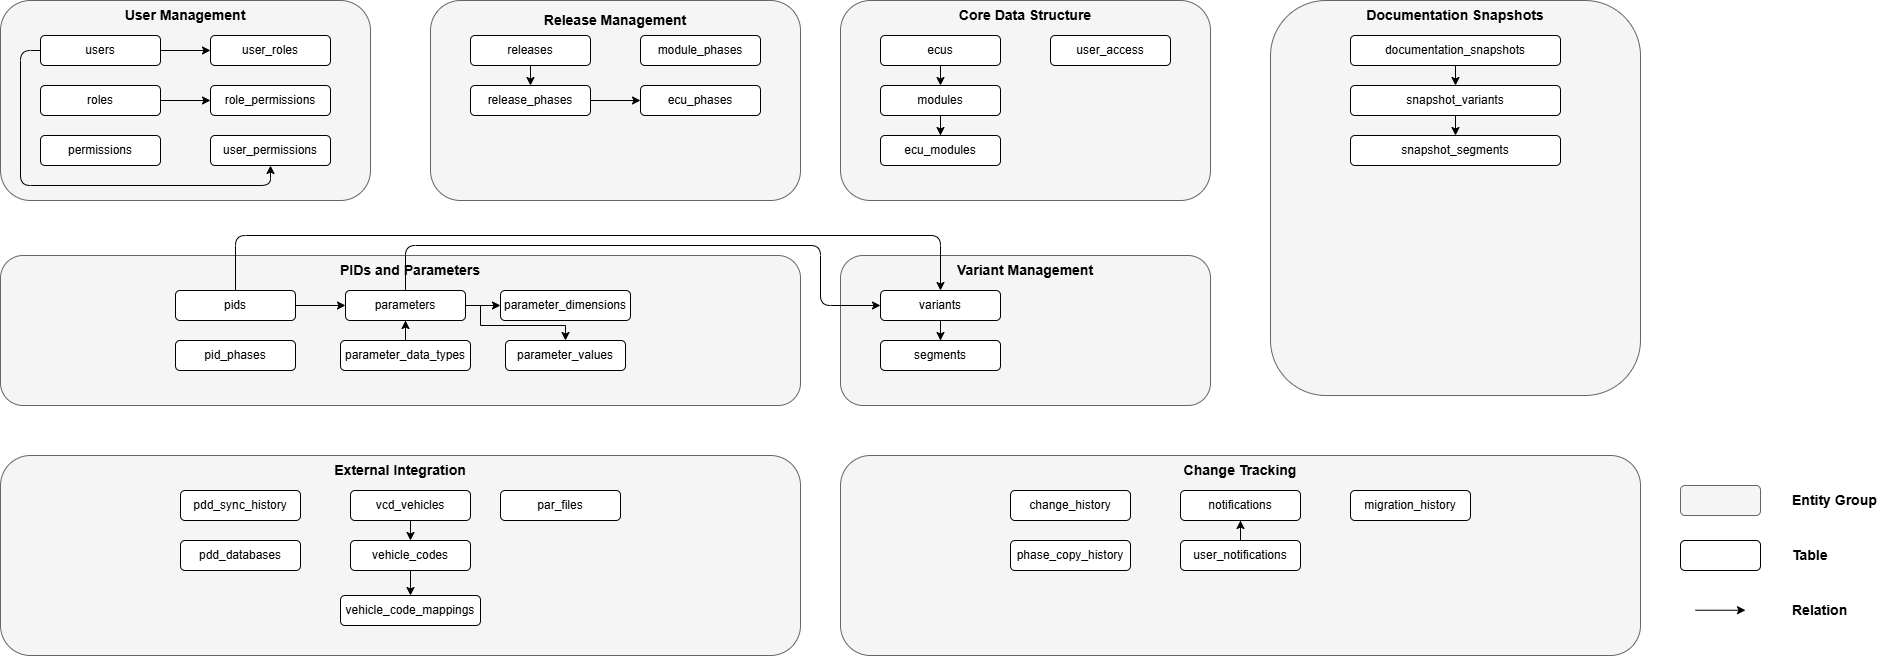
\includegraphics[width=0.95\textwidth]{figures/vmap_er_diagram.png}
    \caption{Entity-Relationship Diagram for VMAP Database}
    \label{fig:er-diagram}
\end{figure}

As shown in Figure \ref{fig:er-diagram}, variant management entities comprise Variants, Segments, and their relationships to parameters, implementing the core parameter customization functionality. Documentation entities include Documentation Snapshots, Snapshot Variants, and Snapshot Segments, supporting preservation of historical parameter states. Integration entities consist of Synchronization Records, Vehicle Configurations, and Parameter File Records, supporting external system connectivity. Finally, audit entities encompass Change History, Transaction Records, and Phase Copy History, providing comprehensive operation traceability.

This model was developed using data normalization principles to minimize redundancy while maintaining data integrity \cite{elmasri2015fundamentals}. Special attention was given to temporal data representation, incorporating bi-temporal database design concepts to track both transaction time and valid time \cite{kulkarni2012temporal}.

\subsection{Temporal Database Consideration}
\label{subsec:temporal-database-consideration}

Considerable attention was given to temporal database concepts as a potential foundation for the version control mechanism. The evaluation focused on bi-temporal modeling \cite{snodgrass1999developing}, which tracks both transaction time (when changes were made) and valid time (when changes are applicable).

% \begin{figure}[htbp]
%     \centering
%     %\includegraphics[width=0.9\textwidth]{figures/temporal_vs_phase_comparison.png}
%     \caption{Comparison of Temporal Database vs. Phase-based Versioning Approach}
%     \label{fig:temporal-comparison}
% \end{figure}

%As shown in Figure \ref{fig:temporal-comparison}, despite potential advantages including comprehensive historical preservation and flexible time-point querying, practical evaluation revealed significant limitations for automotive parameter management. Temporal queries' inherent complexity would introduce overhead potentially impacting interactive performance. The automotive development process organizes around discrete phases rather than continuous time, making the temporal model potentially misaligned with domain concepts. Temporal tables require additional columns and typically more rows to track historical states, substantially increasing storage requirements for a system with millions of parameter values. Effective temporal data querying requires additional indexes, further increasing storage overhead and potentially impacting write performance \cite{bohlen2018database}.
Despite potential advantages including comprehensive historical preservation and flexible time-point querying, practical evaluation revealed significant limitations for automotive parameter management. Temporal queries' inherent complexity would introduce overhead potentially impacting interactive performance. The automotive development process organizes around discrete phases rather than continuous time, making the temporal model potentially misaligned with domain concepts. Temporal tables require additional columns and typically more rows to track historical states, substantially increasing storage requirements for a system with millions of parameter values. Effective temporal data querying requires additional indexes, further increasing storage overhead and potentially impacting write performance \cite{bohlen2018database}.

Based on this evaluation, the system adopted an explicit phase-based approach rather than a temporal database model. This approach explicitly represents the phase-based structure of automotive development, making the model more intuitive for domain experts while supporting efficient parameter and variant retrieval without temporal query complexity \cite{bhattacherjee2015principles}. The phase-based approach better matches automotive parameter management's nature, where discrete development phases form the primary organizing principle rather than continuous time.

\subsection{Release/Phase Separation Rationale}
\label{subsec:release-phase-separation}

A key architectural decision was explicitly separating releases and phases into distinct but related entities. Releases represent major planning cycles in automotive development (typically aligned with model years or major updates like "24.1" or "24.3"), serving as organizational containers for development activities. Phases represent specific development process states (Phase1, Phase2, Phase3, and Phase4) occurring in a predictable sequence, reflecting parameter configuration maturity levels \cite{staron2021automotive}.

This separation provides several benefits: flexible release management allowing new releases with their own phase sequences without disrupting existing development; phase sequence standardization for consistent workflows; independent phase progression allowing different ECUs to advance through phases at different rates; simplified queries for common operations; and clear access control definition at either release or phase level.

The database schema implements this through distinct tables with a parent-child relationship. The releases table defines high-level development cycles, while release\_phases defines specific development states within each release with explicit sequencing. This structure enables efficient release-phase hierarchy navigation while maintaining clear semantic separation between these distinct concepts.

\subsection{Database Schema Design}
\label{subsec:database-schema-design}

The database schema translates the conceptual ER model into concrete database structures optimized for VMAP system requirements. PostgreSQL was selected as the underlying database management system due to its robust support for advanced features essential for this application domain, including complex data types (JSON/JSONB), sophisticated indexing mechanisms (including GIN indexes for text search), powerful procedural language (PL/pgSQL), comprehensive transaction support, and extensibility through custom extensions \cite{biriukov2018implementation}.

The schema addresses several key challenges in representing the automotive parameter domain. Parameters are organized hierarchically (ECU → Module → PID → Parameter) through related tables with appropriate foreign key constraints. Multi-dimensional parameters (arrays or matrices of values) are addressed through dedicated tables for parameter dimensions. Instead of traditional temporal database approaches, a phase-based versioning approach associates each parameter, variant, and segment with a specific phase and maintains phase sequence through explicit numbering.

Comprehensive change tracking is implemented through a specialized change history table capturing both old and new values for each change, using JSONB for flexible storage of different entity structures, grouping related changes by transaction, and supporting efficient filtering by entity type, user, and timestamp. This approach balances comprehensive auditing with performance considerations \cite{bhattacherjee2015principles}.

\subsection{Version Control Mechanism}
\label{subsec:version-control-mechanism}

The version control mechanism is central to VMAP, enabling parameter evolution management across different development phases. Unlike traditional version control systems focusing on linear history, VMAP implements a phase-based approach tailored to the automotive development process.

The release phase framework defines a structured parameter versioning approach based on the established automotive development cycle: Phase1 (initial definition and configuration), Phase2 (adjustments based on initial testing), Phase3 (refinement based on extended testing), and Phase4 (completed configuration ready for production).

This framework is implemented through table structures and procedural logic. Each phase is a distinct database entity associated with releases through a parent-child relationship. Parameters, variants, and segments are tagged with their corresponding phase, enabling explicit versioning without temporal database approach overhead. Explicit phase sequence numbers enable orderly progression, supporting both the development workflow and database operations propagating changes between phases.

The phase transition mechanism handles parameter configuration copying from one phase to the next through a specialized stored procedure. This approach provides several advantages: phases can be modified independently after copying; changes can be propagated forward selectively; each phase maintains a complete parameter configuration; and historical phase data remains accessible indefinitely.

A phase freezing mechanism supports documentation and regulatory compliance. When a phase is frozen, all parameters, variants, and segments become read-only, the frozen state is recorded with timestamp and user information, documentation snapshots are automatically generated, and the change is logged. This ensures significant development milestone configurations are preserved while allowing development to continue in subsequent phases.

\subsection{Parameter Definition Database Synchronization}
\label{subsec:parameter-db-sync}

Parameter Definition Database (CDI) synchronization presented complex architectural challenges. Initially, a version-based approach was considered, tracking parameter changes across releases by storing release information at synchronization. The system would dynamically construct appropriate parameter sets by evaluating parameter version histories. This approach offered theoretical storage efficiency advantages by maintaining only parameter changes rather than complete sets for each release \cite{bhattacherjee2015principles}.

\begin{figure}[htbp]
    \centering
    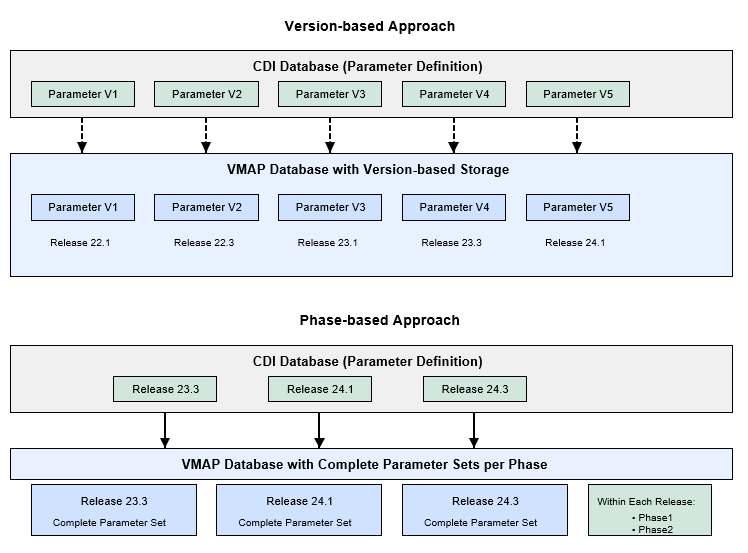
\includegraphics[width=0.9\textwidth]{figures/param-sync-approaches.png}
    \caption{Comparison of Version-based vs. Phase-based Parameter Synchronization Approaches}
    \label{fig:param-sync-approaches}
\end{figure}

Figure \ref{fig:param-sync-approaches} illustrates the comparison between the initially considered version-based approach and the implemented phase-based approach. Detailed analysis revealed significant challenges with versioning. Complex relationships between parameters and their parent entities would require sophisticated versioning logic for the entire hierarchy. Reconstructing parameter sets would require multiple joins across version tables and complex temporal predicates, potentially degrading system responsiveness. Additionally, version-based synchronization would complicate phase inheritance implementation \cite{kulkarni2012temporal}.

After evaluation, a phase-based synchronization approach was adopted instead. This design maintains complete parameter sets for each ECU in each release phase, rather than tracking individual parameter versions across releases. This simplifies query patterns by establishing direct relationships between parameters and their release phases, enables efficient retrieval without complex version reconstruction, aligns naturally with the automotive development process, provides clearer traceability between parameter versions across phases, and offers greater resilience against synchronization failures \cite{hohpe2002enterprise}.

While this approach consumes more storage than a version-based approach, detailed analysis indicated storage requirements remained within acceptable limits, with performance benefits and simplified implementation outweighing additional storage costs.

\section{Validation Mechanisms}
\label{sec:validation-mechanisms}

To ensure data integrity and consistency, VMAP implements multiple validation mechanism layers from basic constraints to sophisticated business rule validation. These layers work together to maintain parameter data quality and reliability throughout the system lifecycle.

\subsection{Data Integrity Constraints}
\label{subsec:data-integrity-constraints}

Database-level constraints enforce basic integrity rules: primary key constraints ensure unique entity identifiers; foreign key constraints maintain referential integrity between related entities; not-null constraints ensure required fields contain values; unique constraints prevent duplicate values in specified columns; and check constraints enforce domain-specific rules such as valid date ranges and parameter value ranges. These constraints are designed into the database schema as integral parts of entity definitions, ensuring consistent enforcement throughout the system \cite{elmasri2015fundamentals}.

\subsection{Business Rule Validation}
\label{subsec:business-rule-validation}

Domain-specific business rules are implemented through database triggers and stored procedures. Parameter range validation automatically checks modified values against defined minimum and maximum bounds, rejecting values outside allowed ranges—critical for automotive parameter management where incorrect values could impact vehicle safety or performance \cite{staron2021automotive}.

Phase status validation prevents frozen phase modification, ensuring historical parameter configuration integrity. Segment validation ensures segments reference valid parameters and variants, contain appropriate dimensional values, and maintain consistent entity relationships. User access validation ensures users can only modify parameters, variants, and segments for modules to which they have been granted access, maintaining data security and integrity in multi-user enterprise systems \cite{sandhu1998role}.

\subsection{Conflict Resolution Strategies}
\label{subsec:conflict-resolution-strategies}

In a multi-user environment, concurrent modifications can create conflicts. VMAP implements several strategies to detect and resolve these, maintaining data consistency while supporting collaborative parameter management. For web-based interactions, optimistic concurrency control using version timestamps allows multiple users to view the same data concurrently, detecting conflicts only when updates collide \cite{bhattacherjee2015principles}.

When changes propagate from one phase to the next, conflicts can arise if the target phase has already been modified. Explicit conflict resolution mechanisms compare the source variant or segment with existing target configurations during phase propagation operations. When conflicts are detected, resolution options allow users to make informed decisions: override the target with source values, preserve target values, or merge values based on specified rules.

Complex operations modifying multiple related entities use explicit transactions to maintain data consistency. Database transactions ensure related modification sets either complete entirely or fail without partial changes. For operations spanning multiple transactions or requiring user interaction, application-level coordination through transaction identifiers and session state enables complex workflows requiring user input while maintaining logical data consistency.

\subsection{Audit and Traceability Mechanisms}
\label{subsec:audit-mechanisms}

Comprehensive audit and traceability mechanisms are essential for regulatory compliance and quality assurance. VMAP includes robust audit capabilities tracking all significant operations while minimizing performance impact. The core is the change history tracking mechanism, automatically capturing both before and after states for entity modifications. For each change, the system records the entity being modified, change type, user, timestamp, and detailed before/after values \cite{bhattacherjee2015principles}.

\begin{figure}[h]
    \centering
    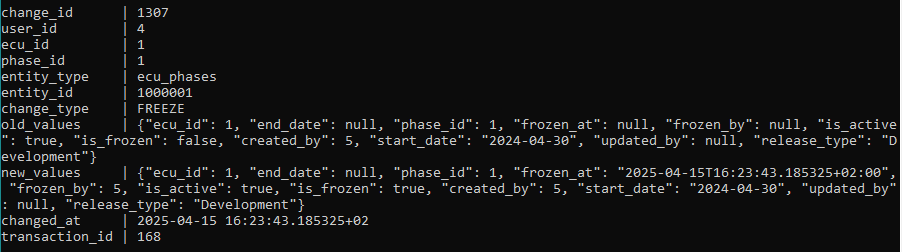
\includegraphics[width=0.95\textwidth]{figures/freeze_audit_trail.png}
    \caption{Audit Trail for Phase Freeze Operation}
    \label{fig:freeze-audit-trail}
\end{figure}

Figure \ref{fig:freeze-audit-trail} shows an example of the audit trail for a phase freeze operation, demonstrating the comprehensive tracking of significant system events. To optimize performance, the audit system selectively filters change data, excluding non-essential fields such as timestamps and large binary data. Additionally, asynchronous audit recording for bulk operations reduces performance impact on high-volume operations while ensuring all changes are eventually recorded.

Beyond change tracking, specialized audit mechanisms address specific scenarios: phase transition logging records all phase propagation operations; freeze operation logging records phase freeze and unfreeze operations; user access logging captures authentication and authorization events; and integration operation logging records all external system interactions.

    \cleardoublepage
    \chapter{Implementation}
\label{chap:implementation}

This chapter presents the technical implementation of the \ac{VMAP} system conceptual architecture described in Chapter \ref{chap:methodology}. The discussion focuses on key architectural components and technical decisions that enable efficient parameter versioning in automotive software development, with concrete implementation details demonstrating how theoretical concepts translate to practical solutions.

\section{Database Structure Implementation}
\label{sec:database-structure-implementation}

Following the comparative analysis of database systems presented in Chapter \ref{chap:methodology}, PostgreSQL was selected as the implementation platform due to its superior support for complex data types, extensibility features, and advanced indexing capabilities \cite{obe2017postgresql}. The database implementation transforms abstract entities and relationships into concrete database structures, implementing the hierarchical organization of automotive electronic systems through physical tables and relationships.

\subsection{Core Data Entities}
\label{subsec:core-data-entities}

The hierarchical structure of automotive electronic systems is implemented through four primary entity types: \acp{ECU}, Modules, \acp{PID}, and Parameters. The \ac{ECU} and Module entities form the top levels of the hierarchy, with a many-to-many relationship reflecting the reality that modules can exist across multiple \acp{ECU}. This structure aligns with the domain model described by Staron \cite{staron2021automotive}, where logical groupings of software functions must be maintained across different hardware configurations.

\begin{lstlisting}[language=SQL, caption={ECU and Module Table Implementation}, label={lst:ecu-module-tables}]
CREATE TABLE ecus (
    ecu_id INTEGER PRIMARY KEY,
    name VARCHAR(100) NOT NULL,
    description TEXT,
    byte_order VARCHAR(50),
    created_at TIMESTAMP WITH TIME ZONE DEFAULT CURRENT_TIMESTAMP,
    external_id INTEGER UNIQUE -- \ac{PDD}reference ID
);

CREATE TABLE modules (
    module_id INTEGER PRIMARY KEY,
    shortcut VARCHAR(50) NOT NULL,
    name VARCHAR(255) NOT NULL,
    kind VARCHAR(255),
    created_at TIMESTAMP WITH TIME ZONE DEFAULT CURRENT_TIMESTAMP,
    external_id INTEGER UNIQUE -- \ac{PDD}reference ID
);

CREATE TABLE ecu_modules (
    ecu_id INTEGER REFERENCES ecus(ecu_id) ON DELETE CASCADE,
    module_id INTEGER REFERENCES modules(module_id) ON DELETE CASCADE,
    created_at TIMESTAMP WITH TIME ZONE DEFAULT CURRENT_TIMESTAMP,
    PRIMARY KEY (ecu_id, module_id)
);
\end{lstlisting}

The junction table \texttt{ecu\_modules} implements the many-to-many relationship using foreign key constraints as described by Elmasri and Navathe \cite{elmasri2015fundamentals}. Each entity includes an \texttt{external\_id} attribute to maintain mapping with the Parameter Definition Database (PDD), facilitating integration through persistent identifier correlation as recommended by Hohpe and Woolf \cite{hohpe2002enterprise}.

\acp{PID} and parameters constitute the lower levels of the hierarchy, with PIDs grouping related parameters for specific modules. The parameter table implements additional attributes for handling the complexity of automotive parameter specifications:

\begin{lstlisting}[language=SQL, caption={Parameter Table Implementation}, label={lst:parameter-table}]
CREATE TABLE parameters (
    parameter_id BIGINT PRIMARY KEY,
    pid_id BIGINT REFERENCES pids(pid_id) ON DELETE CASCADE,
    ecu_id INTEGER,
    phase_id INTEGER,
    name VARCHAR(255) NOT NULL,
    parameter_name VARCHAR(255),
    type_id INTEGER REFERENCES parameter_data_types(data_type_id),
    array_definition VARCHAR(50),
    position INTEGER,
    factor DECIMAL,
    unit VARCHAR(50),
    bias_offset DECIMAL,
    is_active BOOLEAN DEFAULT true,
    external_id INTEGER, -- \ac{PDD}reference ID
    FOREIGN KEY (ecu_id, phase_id) REFERENCES ecu_phases(ecu_id, phase_id)
);
\end{lstlisting}

The parameter table incorporates a form of strategic denormalization by including direct references to \texttt{ecu\_id} and \texttt{phase\_id} alongside the \ac{PID} foreign key. While this introduces some redundancy, this approach aims to improve query execution for parameter queries filtered by release phase, a critical operation in the system. Bhattacherjee et al. \cite{bhattacherjee2015principles} note that such denormalization can be justified when query performance benefits outweigh the overhead of maintaining consistency, especially for frequently accessed paths in the data model.

A particularly challenging aspect of the implementation was supporting multi-dimensional parameters, which are common in automotive applications for representing lookup tables and characteristic curves \cite{kiencke2000automotive}. This was addressed through a specialized table structure:

\begin{lstlisting}[language=SQL, caption={Parameter Dimension Implementation}, label={lst:parameter-dimension}]
CREATE TABLE parameter_dimensions (
    dimension_id BIGINT PRIMARY KEY,
    parameter_id BIGINT REFERENCES parameters(parameter_id) ON DELETE CASCADE,
    dimension_index INTEGER NOT NULL,
    default_value NUMERIC NOT NULL,
    external_id INTEGER, -- \ac{PDD}reference ID
    UNIQUE (parameter_id, dimension_index)
);
\end{lstlisting}

This implementation follows a modified entity-attribute-value (EAV) pattern while addressing the potential challenges typically associated with such models \cite{dinu2007guidelines}. The introduction of a dimension index provides an ordered structure to parameter dimensions, enabling efficient representation of arrays and matrices while maintaining the relationship between parameters and their dimensional values.

\subsection{Version Control Implementation}
\label{subsec:version-control-implementation}

The version control implementation is a defining feature of the \ac{VMAP} system, enabling parameter evolution management across different development phases. After evaluating multiple approaches described in Chapter \ref{chap:methodology}, the phase-based versioning model was implemented, creating explicit relationships between parameters and development phases rather than using a generic temporal approach.

\begin{lstlisting}[language=SQL, caption={Release and Phase Management Implementation}, label={lst:release-phase-tables}]
CREATE TABLE releases (
    release_id INTEGER PRIMARY KEY,
    name VARCHAR(50) NOT NULL UNIQUE, -- e.g., "24.1", "24.3"
    description TEXT,
    is_active BOOLEAN DEFAULT true,
    created_at TIMESTAMP WITH TIME ZONE DEFAULT CURRENT_TIMESTAMP,
    created_by BIGINT REFERENCES users(user_id)
);

CREATE TABLE release_phases (
    phase_id INTEGER PRIMARY KEY,
    release_id INTEGER REFERENCES releases(release_id) ON DELETE CASCADE,
    name VARCHAR(50) NOT NULL, -- e.g., "Initial", "PreTest1", "PreTest2", "Final"
    sequence_number INTEGER NOT NULL, -- Determines the order of phases
    is_active BOOLEAN DEFAULT true,
    created_at TIMESTAMP WITH TIME ZONE DEFAULT CURRENT_TIMESTAMP,
    created_by BIGINT REFERENCES users(user_id),
    UNIQUE (release_id, name),
    UNIQUE (release_id, sequence_number)
);

CREATE TABLE ecu_phases (
    ecu_id INTEGER REFERENCES ecus(ecu_id) ON DELETE CASCADE,
    phase_id INTEGER REFERENCES release_phases(phase_id) ON DELETE CASCADE,
    is_active BOOLEAN DEFAULT true,
    is_frozen BOOLEAN DEFAULT false,
    frozen_at TIMESTAMP WITH TIME ZONE,
    frozen_by BIGINT REFERENCES users(user_id),
    created_at TIMESTAMP WITH TIME ZONE DEFAULT CURRENT_TIMESTAMP,
    created_by BIGINT REFERENCES users(user_id),
    PRIMARY KEY (ecu_id, phase_id)
);
\end{lstlisting}

This implementation supports the bi-annual release cycle with four sequential phases per release. The \texttt{sequence\_number} field provides explicit ordering of phases within a release, while unique constraints ensure consistency of phase naming and sequencing. The ECU-phase mapping implements the association between ECUs and specific release phases, supporting independent progression of different ECUs through the development cycle as described by Broy \cite{broy2006challenges}.

The phase-based approach was selected over temporal versioning for several reasons supported by database design principles:

\begin{itemize}
    \item Direct phase associations align with the process-based nature of automotive development, where parameters evolve through explicitly defined development stages.
    \item The explicit phase relationships simplify the implementation of phase transitions and comparison operations, which are fundamental to the automotive development process as described by Pretschner et al. \cite{pretschner2007software}.
    \item The approach aligns with the mental model of automotive development engineers, who conceptualize parameter evolution in terms of distinct development phases rather than continuous time.
\end{itemize}

Phase management functionality was implemented through a stored procedure for phase transitions and parameter propagation:

\begin{lstlisting}[language=SQL, caption={Phase Transition Function}, label={lst:phase-transition}]
CREATE OR REPLACE FUNCTION copy_phase_data(
    source_ecu_id INTEGER,
    source_phase_id INTEGER,
    target_ecu_id INTEGER,
    target_phase_id INTEGER,
    user_id BIGINT
)
RETURNS TABLE (
    variants_copied INTEGER,
    segments_copied INTEGER
) AS $$
DECLARE
    variant_count INTEGER := 0;
    segment_count INTEGER := 0;
    transaction_id BIGINT;
BEGIN
    -- Get a transaction ID for change tracking
    SELECT nextval('change_history_transaction_id_seq') INTO transaction_id;
    
    -- Set the transaction ID for tracking in logging trigger
    PERFORM set_config('app.transaction_id', transaction_id::text, true);
    PERFORM set_config('app.user_id', user_id::text, true);
    
    -- Create a temporary table to map source variant IDs to target variant IDs
    CREATE TEMPORARY TABLE variant_mapping (
        source_variant_id BIGINT,
        target_variant_id BIGINT
    ) ON COMMIT DROP;
    
    -- Copy variants with modified attributes for target phase
    WITH inserted_variants AS (
        INSERT INTO variants (
            pid_id, ecu_id, phase_id, name, code_rule, 
            created_at, created_by, updated_by
        )
        SELECT 
            v.pid_id, target_ecu_id, target_phase_id, v.name, v.code_rule,
            CURRENT_TIMESTAMP, user_id, user_id
        FROM variants v
        WHERE v.ecu_id = source_ecu_id AND v.phase_id = source_phase_id
        RETURNING variant_id, pid_id, name, code_rule
    )
    INSERT INTO variant_mapping (source_variant_id, target_variant_id)
    SELECT v.variant_id, iv.variant_id
    FROM variants v
    JOIN inserted_variants iv ON v.pid_id = iv.pid_id 
                             AND v.name = iv.name 
                             AND v.code_rule = iv.code_rule
    WHERE v.ecu_id = source_ecu_id AND v.phase_id = source_phase_id;
    
    -- Get count of copied variants
    SELECT COUNT(*) INTO variant_count FROM variant_mapping;
    
    -- Copy segments with parameter mapping
    -- [Additional implementation details omitted for brevity]
    
    RETURN QUERY SELECT variant_count, segment_count;
END;
$$ LANGUAGE plpgsql;
\end{lstlisting}

This implementation provides an atomic transaction for phase transition, copying parameter variants and segments from one phase to another while maintaining proper references and tracking the operation in the change history. The function returns counts of affected entities, providing immediate feedback on the operation's scope. The use of temporary tables for mapping entities between phases implements the identity map pattern described by Fowler \cite{fowler2003patterns}, ensuring proper relationship preservation during complex operations.

\subsection{Variant and Segment Management}
\label{subsec:variant-segment-management}

The variant and segment management implementation realizes the core parameter customization capabilities of the \ac{VMAP} system:

\begin{lstlisting}[language=SQL, caption={Variant and Segment Implementation}, label={lst:variant-segment-tables}]
CREATE TABLE variants (
    variant_id BIGINT PRIMARY KEY,
    pid_id BIGINT REFERENCES pids(pid_id) ON DELETE CASCADE,
    ecu_id INTEGER,
    phase_id INTEGER,
    name VARCHAR(100) NOT NULL,
    code_rule TEXT,
    created_at TIMESTAMP WITH TIME ZONE DEFAULT CURRENT_TIMESTAMP,
    created_by BIGINT REFERENCES users(user_id),
    updated_by BIGINT REFERENCES users(user_id),
    FOREIGN KEY (ecu_id, phase_id) REFERENCES ecu_phases(ecu_id, phase_id),
    UNIQUE (phase_id, pid_id, name),
    UNIQUE (phase_id, pid_id, code_rule)
);

CREATE TABLE segments (
    segment_id BIGINT PRIMARY KEY,
    variant_id BIGINT REFERENCES variants(variant_id) ON DELETE CASCADE,
    parameter_id BIGINT REFERENCES parameters(parameter_id) ON DELETE CASCADE,
    dimension_index INTEGER NOT NULL,
    decimal NUMERIC NOT NULL,
    created_at TIMESTAMP WITH TIME ZONE DEFAULT CURRENT_TIMESTAMP,
    created_by BIGINT REFERENCES users(user_id),
    updated_by BIGINT REFERENCES users(user_id)
);
\end{lstlisting}

Each variant is associated with a specific PID, ECU, and phase, creating a three-way relationship that places the variant in both functional and temporal contexts. The uniqueness constraints prevent duplicate variant names or code rules within the same \ac{PID} and phase, enforcing a critical business rule identified during requirements analysis. The \texttt{code\_rule} field stores boolean expressions determining when a variant applies based on vehicle configuration codes, implementing a domain-specific rule language for variant applicability.

Segments form the foundation of parameter customization, linking parameters to variants and storing modified values. The canonical decimal representation for all parameter values, regardless of native data type, implements the canonical model pattern described by Hohpe and Woolf \cite{hohpe2002enterprise}, simplifying data manipulation while ensuring consistent value handling.

For parameter value resolution, a specialized database function was implemented:

\begin{lstlisting}[language=SQL, caption={Parameter Resolution Function}, label={lst:parameter-resolution}]
CREATE OR REPLACE FUNCTION resolve_parameter_value(
    p_parameter_id BIGINT,
    p_dimension_index INTEGER,
    p_variant_ids BIGINT[]
)
RETURNS NUMERIC AS $$
DECLARE
    v_value NUMERIC;
    v_default_value NUMERIC;
BEGIN
    -- First try to find a segment with the given parameter and variant
    SELECT s.decimal INTO v_value
    FROM segments s
    WHERE s.parameter_id = p_parameter_id
      AND s.dimension_index = p_dimension_index
      AND s.variant_id = ANY(p_variant_ids)
    ORDER BY array_position(p_variant_ids, s.variant_id)
    LIMIT 1;
    
    -- If no segment found, get the default value
    IF v_value IS NULL THEN
        SELECT pd.default_value INTO v_default_value
        FROM parameter_dimensions pd
        WHERE pd.parameter_id = p_parameter_id
          AND pd.dimension_index = p_dimension_index;
          
        -- If no dimension record, try parameter default
        IF v_default_value IS NULL THEN
            SELECT p.default_value INTO v_default_value
            FROM parameters p
            WHERE p.parameter_id = p_parameter_id;
        END IF;
        
        v_value := COALESCE(v_default_value, 0);
    END IF;
    
    RETURN v_value;
END;
$$ LANGUAGE plpgsql;
\end{lstlisting}

This function implements the value resolution logic required for parameter file generation, handling the complex logic of finding applicable parameter values based on variant precedence. The array position-based ordering ensures that variants are applied in the correct priority sequence, a critical requirement for automotive parameter management as described by Staron \cite{staron2021automotive}.

To support documentation and compliance requirements, a snapshot mechanism was implemented to capture complete parameter configurations at specific points in time:

\begin{lstlisting}[language=SQL, caption={Documentation Snapshot Implementation}, label={lst:documentation-snapshot}]
CREATE TABLE documentation_snapshots (
    snapshot_id INTEGER PRIMARY KEY,
    name VARCHAR(255) NOT NULL,
    description TEXT,
    ecu_id INTEGER,
    phase_id INTEGER,
    variant_count INTEGER DEFAULT 0,
    segment_count INTEGER DEFAULT 0,
    created_at TIMESTAMP WITH TIME ZONE DEFAULT CURRENT_TIMESTAMP,
    created_by BIGINT REFERENCES users(user_id),
    FOREIGN KEY (ecu_id, phase_id) REFERENCES ecu_phases(ecu_id, phase_id)
);

CREATE TABLE snapshot_variants (
    snapshot_variant_id INTEGER PRIMARY KEY,
    snapshot_id INTEGER REFERENCES documentation_snapshots(snapshot_id) ON DELETE CASCADE,
    original_variant_id BIGINT, -- Reference to the original variant
    pid_id BIGINT REFERENCES pids(pid_id) ON DELETE CASCADE,
    name VARCHAR(100) NOT NULL,
    code_rule TEXT,
    created_at TIMESTAMP WITH TIME ZONE,
    created_by BIGINT REFERENCES users(user_id)
);

CREATE TABLE snapshot_segments (
    snapshot_segment_id INTEGER PRIMARY KEY,
    snapshot_id INTEGER REFERENCES documentation_snapshots(snapshot_id) ON DELETE CASCADE,
    snapshot_variant_id INTEGER REFERENCES snapshot_variants(snapshot_variant_id) ON DELETE CASCADE,
    original_segment_id BIGINT, -- Reference to the original segment
    parameter_id BIGINT REFERENCES parameters(parameter_id) ON DELETE CASCADE,
    dimension_index INTEGER NOT NULL,
    decimal NUMERIC NOT NULL,
    created_at TIMESTAMP WITH TIME ZONE,
    created_by BIGINT REFERENCES users(user_id)
);
\end{lstlisting}

This implementation follows the snapshot pattern described by Fowler \cite{fowler2003patterns}, creating a complete copy of variant and segment data at specific points in time. Rather than using a temporal database approach with validity periods, the system explicitly materializes historical states, ensuring they remain accessible regardless of subsequent modifications to live data. References to original entities enable traceability between snapshot and live data, implementing the origin tracking pattern described by Tichy \cite{tichy1985rcs}.

The snapshot creation function automates the process of capturing parameter configurations:

\begin{lstlisting}[language=SQL, caption={Documentation Snapshot Function}, label={lst:documentation-snapshot-function}]
CREATE OR REPLACE FUNCTION create_documentation_snapshot(
    p_name VARCHAR(255),
    p_description TEXT,
    p_ecu_id INTEGER,
    p_phase_id INTEGER,
    p_user_id BIGINT
)
RETURNS INTEGER AS $$
DECLARE
    v_snapshot_id INTEGER;
BEGIN
    -- Create the snapshot record
    INSERT INTO documentation_snapshots (
        name, description, ecu_id, phase_id,
        variant_count, segment_count, created_at, created_by
    ) VALUES (
        p_name, p_description, p_ecu_id, p_phase_id,
        0, 0, CURRENT_TIMESTAMP, p_user_id
    ) RETURNING snapshot_id INTO v_snapshot_id;

    -- Copy all variants for the ECU and phase
    INSERT INTO snapshot_variants (
        snapshot_id, original_variant_id, pid_id, name,
        code_rule, created_at, created_by
    )
    SELECT 
        v_snapshot_id, v.variant_id, v.pid_id, v.name,
        v.code_rule, v.created_at, v.created_by
    FROM variants v
    WHERE v.ecu_id = p_ecu_id AND v.phase_id = p_phase_id;
    
    -- Copy all segments for the variants
    -- [Implementation details omitted for brevity]
    
    -- Update the counts in the snapshot record
    -- [Implementation details omitted for brevity]
    
    RETURN v_snapshot_id;
END;
$$ LANGUAGE plpgsql;
\end{lstlisting}

In the automotive industry, these snapshots serve multiple purposes: providing immutable records of parameter configurations at significant development milestones, supporting quality assurance processes and regulatory compliance requirements, and facilitating comparative analysis between development phases.

\section{Access Control Implementation}
\label{sec:access-control-implementation}

The access control implementation realizes the hybrid role-permission model described in Chapter \ref{chap:methodology}, providing a flexible foundation for managing user permissions across the system.

\subsection{Role-Based Permission Model}
\label{subsec:role-based-permission-model}

The core \ac{RBAC} implementation follows the structure defined by Sandhu et al. \cite{sandhu1998role}, with tables for users, roles, permissions, and their relationships:

\begin{lstlisting}[language=SQL, caption={Core RBAC Implementation}, label={lst:rbac-implementation}]
CREATE TABLE roles (
    role_id INTEGER PRIMARY KEY,
    name VARCHAR(255) UNIQUE NOT NULL,
    description TEXT
);

CREATE TABLE permissions (
    permission_id INTEGER PRIMARY KEY,
    name VARCHAR(255) UNIQUE NOT NULL,
    description TEXT
);

CREATE TABLE role_permissions (
    role_id INTEGER REFERENCES roles(role_id) ON DELETE CASCADE,
    permission_id INTEGER REFERENCES permissions(permission_id) ON DELETE CASCADE,
    granted_at TIMESTAMP WITH TIME ZONE DEFAULT CURRENT_TIMESTAMP,
    granted_by BIGINT REFERENCES users(user_id),
    PRIMARY KEY (role_id, permission_id)
);

CREATE TABLE user_roles (
    user_id BIGINT REFERENCES users(user_id) ON DELETE CASCADE,
    role_id INTEGER REFERENCES roles(role_id) ON DELETE CASCADE,
    granted_at TIMESTAMP WITH TIME ZONE DEFAULT CURRENT_TIMESTAMP,
    granted_by BIGINT REFERENCES users(user_id),
    PRIMARY KEY (user_id, role_id)
);
\end{lstlisting}

The model is extended with direct user permissions to implement the hybrid approach:

\begin{lstlisting}[language=SQL, caption={User-Permission Implementation}, label={lst:user-permission}]
CREATE TABLE user_permissions (
    user_permission_id INTEGER PRIMARY KEY,
    user_id BIGINT REFERENCES users(user_id) ON DELETE CASCADE,
    permission_id INTEGER REFERENCES permissions(permission_id) ON DELETE CASCADE,
    granted_by BIGINT REFERENCES users(user_id),
    granted_at TIMESTAMP WITH TIME ZONE DEFAULT CURRENT_TIMESTAMP,
    UNIQUE (user_id, permission_id)
);
\end{lstlisting}

This hybrid model allows permissions to be granted either through role assignments or directly to users, providing the flexibility to handle exceptional cases without creating specialized roles, as recommended by Ferraiolo et al. \cite{ferraiolo2011policy}.

The permission checking function implements the core security verification logic:

\begin{lstlisting}[language=SQL, caption={Permission Check Implementation}, label={lst:permission-check}]
CREATE OR REPLACE FUNCTION has_permission(
    p_user_id BIGINT,
    p_permission_name VARCHAR
)
RETURNS BOOLEAN AS $$
BEGIN
    RETURN EXISTS (
        -- Check role-based permissions
        SELECT 1
        FROM user_roles ur
        JOIN role_permissions rp ON ur.role_id = rp.role_id
        JOIN permissions p ON rp.permission_id = p.permission_id
        WHERE ur.user_id = p_user_id AND p.name = p_permission_name
        
        UNION
        
        -- Check direct user permissions
        SELECT 1
        FROM user_permissions up
        JOIN permissions p ON up.permission_id = p.permission_id
        WHERE up.user_id = p_user_id AND p.name = p_permission_name
    );
END;
$$ LANGUAGE plpgsql;
\end{lstlisting}

The UNION-based approach combines role-based and direct permission checks in a single database query, implementing an efficient verification mechanism. This implementation supports the separation of permission checking from application logic, allowing security policies to be enforced consistently across different access paths.

\subsection{Module-Based Access Control}
\label{subsec:module-based-access-control}

To complement the role-based permission model, a module-based access control system was implemented to restrict write access based on module assignments:

\begin{lstlisting}[language=SQL, caption={Module Access Control Implementation}, label={lst:module-access}]
CREATE TABLE user_access (
    user_id BIGINT REFERENCES users(user_id) ON DELETE CASCADE,
    ecu_id INTEGER REFERENCES ecus(ecu_id) ON DELETE CASCADE,
    module_id INTEGER REFERENCES modules(module_id) ON DELETE CASCADE,
    write_access BOOLEAN DEFAULT true,
    created_at TIMESTAMP WITH TIME ZONE DEFAULT CURRENT_TIMESTAMP,
    created_by BIGINT REFERENCES users(user_id),
    PRIMARY KEY (user_id, ecu_id, module_id),
    CONSTRAINT user_access_ecu_module_fk FOREIGN KEY (ecu_id, module_id) 
    REFERENCES ecu_modules(ecu_id, module_id)
);
\end{lstlisting}

This implementation establishes a three-way relationship between users, ECUs, and modules, with a boolean flag distinguishing between read and write access. The constraint ensures access is granted only for valid ECU-module combinations, enforcing structural integrity. Database functions verify both role-based permissions and module-based access rights during critical operations:

\begin{lstlisting}[language=SQL, caption={Module Access Check Implementation}, label={lst:module-access-check}]
CREATE OR REPLACE FUNCTION has_module_write_access(
    p_user_id BIGINT,
    p_ecu_id INTEGER,
    p_module_id INTEGER
)
RETURNS BOOLEAN AS $$
BEGIN
    -- First check if user has administrator role (bypasses module restrictions)
    IF EXISTS (
        SELECT 1
        FROM user_roles ur
        JOIN roles r ON ur.role_id = r.role_id
        WHERE ur.user_id = p_user_id AND r.name = 'administrator'
    ) THEN
        RETURN TRUE;
    END IF;
    
    -- Check module-specific write access
    RETURN EXISTS (
        SELECT 1
        FROM user_access ua
        WHERE ua.user_id = p_user_id
          AND ua.ecu_id = p_ecu_id
          AND ua.module_id = p_module_id
          AND ua.write_access = TRUE
    );
END;
$$ LANGUAGE plpgsql;
\end{lstlisting}

This implementation combines role-based and attribute-based access control approaches, creating what Ferraiolo et al. describe as policy-enhanced \ac{RBAC} \cite{ferraiolo2011policy}. The function first checks for administrator privileges, which bypass module-specific restrictions, then verifies specific module access rights if necessary.

\section{Query Optimization Implementation}
\label{sec:query-optimization-implementation}

The complex relationships and large data volumes in automotive parameter management necessitated a comprehensive indexing strategy to support common query patterns.

\subsection{Indexing Implementation}
\label{subsec:indexing-implementation}

The indexing strategy focuses on accelerating hierarchical navigation and parameter retrieval operations:

\begin{lstlisting}[language=SQL, caption={Core Index Implementation}, label={lst:core-indexes}]
-- Hierarchical path indexes
CREATE INDEX idx_pids_ecu_module ON pids(ecu_id, module_id);
CREATE INDEX idx_parameters_pid_phase ON parameters(pid_id, phase_id);
CREATE INDEX idx_variants_pid_phase ON variants(pid_id, phase_id);
CREATE INDEX idx_segments_variant ON segments(variant_id);
CREATE INDEX idx_segments_parameter ON segments(parameter_id);

-- Phase-specific indexes
CREATE INDEX idx_parameters_phase ON parameters(phase_id);
CREATE INDEX idx_variants_phase ON variants(phase_id);

-- Text search optimization
CREATE EXTENSION IF NOT EXISTS pg_trgm;
CREATE INDEX idx_parameters_name_trgm 
    ON parameters USING gin (name gin_trgm_ops);
CREATE INDEX idx_variants_name_trgm 
    ON variants USING gin (name gin_trgm_ops);
\end{lstlisting}

These indexes match the natural navigation paths in the data model, implementing the access path optimization pattern described by Molinaro \cite{molinaro2005sql}. The hierarchical path indexes support efficient traversal from ECUs through modules and PIDs to parameters, while the phase-specific indexes accelerate queries filtered by release phase, a common operation in the system.

The trigram-based text search indexes utilize PostgreSQL's specialized text search capabilities as described by Obe and Hsu \cite{obe2017postgresql}. These indexes enable efficient pattern matching and similarity-based searches, accommodating the fuzzy search requirements identified during user interviews. According to Karwin \cite{karwin2010sql}, these specialized indexes can significantly improve the performance of text-based queries, which are common in parameter management systems where engineers need to locate parameters by name or partial name.

\subsection{Function-Based Optimization}
\label{subsec:function-based-optimization}

To optimize complex parameter retrieval operations, several specialized database functions were implemented:

\begin{lstlisting}[language=SQL, caption={Parameter Search Function}, label={lst:parameter-search}]
CREATE OR REPLACE FUNCTION search_parameters(
    search_term TEXT,
    max_results INT DEFAULT 20,
    ecu_id_filter INT DEFAULT NULL,
    phase_id_filter INT DEFAULT NULL
)
RETURNS TABLE (
    parameter_id BIGINT,
    name VARCHAR,
    parameter_name VARCHAR, 
    pid_id BIGINT,
    pid_name VARCHAR,
    module_id INTEGER,
    module_name VARCHAR,
    ecu_id INTEGER,
    ecu_name VARCHAR,
    phase_id INTEGER,
    relevance REAL
) AS $$
BEGIN
  RETURN QUERY
  SELECT 
    p.parameter_id,
    p.name,
    p.parameter_name,
    pid.pid_id,
    pid.name AS pid_name,
    m.module_id,
    m.name AS module_name,
    e.ecu_id,
    e.name AS ecu_name,
    p.phase_id,
    -- Calculate relevance score based on different matching criteria
    (CASE 
        -- Exact matches get highest score
        WHEN p.name ILIKE search_term OR p.parameter_name ILIKE search_term THEN 1.0
        -- Starts with gets high score
        WHEN p.name ILIKE (search_term || '%') OR p.parameter_name ILIKE (search_term || '%') THEN 0.8
        -- Contains gets medium score
        ELSE GREATEST(
            similarity(p.name, search_term),
            similarity(p.parameter_name, search_term)
        )
    END) AS relevance
  FROM 
    parameters p
  JOIN 
    pids\ac{PID}ON p.pid_id = pid.pid_id
  JOIN 
    modules m ON pid.module_id = m.module_id
  JOIN 
    ecus e ON pid.ecu_id = e.ecu_id
  WHERE 
    -- Apply filters if provided
    (ecu_id_filter IS NULL OR e.ecu_id = ecu_id_filter) AND
    (phase_id_filter IS NULL OR p.phase_id = phase_id_filter) AND
    -- Match parameter name or display name
    (p.name ILIKE '%' || search_term || '%' OR 
     p.parameter_name ILIKE '%' || search_term || '%') AND
    -- Only active parameters
    p.is_active = true
  ORDER BY 
    relevance DESC, 
    p.name ASC
  LIMIT max_results;
END;
$$ LANGUAGE plpgsql;
\end{lstlisting}

This function implements a sophisticated parameter search algorithm that combines exact matches, prefix matches, and similarity-based matching to provide relevant search results. The relevance scoring approach ensures that the most relevant parameters appear first in the results, following the information retrieval principles described by Obe and Hsu \cite{obe2017postgresql}.

For phase comparison operations, a specialized function implements the parameter difference detection logic:

\begin{lstlisting}[language=SQL, caption={Phase Comparison Function}, label={lst:phase-comparison}]
CREATE OR REPLACE FUNCTION get_pids_with_changes_between_phases(
    p_ecu_id INTEGER,
    p_module_id INTEGER,
    p_source_phase_id INTEGER,
    p_target_phase_id INTEGER
)
RETURNS TABLE (
    pid_id BIGINT,
    name VARCHAR,
    has_param_changes BOOLEAN,
    has_variant_changes BOOLEAN,
    has_segment_changes BOOLEAN
) AS $
BEGIN
    RETURN QUERY
    WITH common_pids AS (
        -- Get PIDs available in at least one of the phases
        SELECT DISTINCT p.pid_id, p.name
        FROM pids p
        LEFT JOIN pid_phases pp1 ON p.pid_id = pp1.pid_id AND pp1.phase_id = p_source_phase_id
        LEFT JOIN pid_phases pp2 ON p.pid_id = pp2.pid_id AND pp2.phase_id = p_target_phase_id
        WHERE p.ecu_id = p_ecu_id AND p.module_id = p_module_id
          AND (pp1.phase_id IS NOT NULL OR pp2.phase_id IS NOT NULL)
    ),
    -- Parameter changes detection
    param_changes AS (
        SELECT cp.pid_id
        FROM common_pids cp
        WHERE EXISTS (
            -- Parameters that exist in target but not in source
            SELECT 1 FROM parameters pt
            WHERE pt.pid_id = cp.pid_id
              AND pt.phase_id = p_target_phase_id
              AND NOT EXISTS (
                  SELECT 1 FROM parameters ps
                  WHERE ps.pid_id = cp.pid_id
                    AND ps.phase_id = p_source_phase_id
                    AND ps.external_id = pt.external_id
              )
        ) OR EXISTS (
            -- Parameters that exist in source but not in target
            SELECT 1 FROM parameters ps
            WHERE ps.pid_id = cp.pid_id
              AND ps.phase_id = p_source_phase_id
              AND NOT EXISTS (
                  SELECT 1 FROM parameters pt
                  WHERE pt.pid_id = cp.pid_id
                    AND pt.phase_id = p_target_phase_id
                    AND pt.external_id = ps.external_id
              )
        ) OR EXISTS (
            -- Parameters that exist in both but have differences
            SELECT 1 FROM parameters ps
            JOIN parameters pt ON ps.external_id = pt.external_id
            WHERE ps.pid_id = cp.pid_id
              AND pt.pid_id = cp.pid_id
              AND ps.phase_id = p_source_phase_id
              AND pt.phase_id = p_target_phase_id
              AND (
                  ps.name != pt.name OR
                  ps.parameter_name != pt.parameter_name OR
                  ps.type_id != pt.type_id OR
                  ps.factor != pt.factor OR
                  ps.bias_offset != pt.bias_offset OR
                  ps.unit != pt.unit
              )
        )
    ),
    -- Variant changes detection
    variant_changes AS (
        SELECT cp.pid_id
        FROM common_pids cp
        WHERE EXISTS (
            -- Different variant counts between phases
            SELECT 1
            FROM (
                SELECT pid_id, count(*) as cnt
                FROM variants
                WHERE pid_id = cp.pid_id AND phase_id = p_source_phase_id
                GROUP BY pid_id
                
                UNION ALL
                
                SELECT pid_id, -count(*) as cnt
                FROM variants
                WHERE pid_id = cp.pid_id AND phase_id = p_target_phase_id
                GROUP BY pid_id
            ) v
            GROUP BY v.pid_id
            HAVING sum(v.cnt) != 0
        ) OR EXISTS (
            -- Variants with same name but different code rules
            SELECT 1
            FROM variants vs
            JOIN variants vt ON vs.name = vt.name
            WHERE vs.pid_id = cp.pid_id
              AND vt.pid_id = cp.pid_id
              AND vs.phase_id = p_source_phase_id
              AND vt.phase_id = p_target_phase_id
              AND vs.code_rule != vt.code_rule
        )
    ),
    -- Segment changes detection
    segment_changes AS (
        SELECT cp.pid_id
        FROM common_pids cp
        JOIN parameters ps ON ps.pid_id = cp.pid_id AND ps.phase_id = p_source_phase_id
        JOIN parameters pt ON pt.pid_id = cp.pid_id AND pt.phase_id = p_target_phase_id
                         AND pt.external_id = ps.external_id
        JOIN variants vs ON vs.pid_id = cp.pid_id AND vs.phase_id = p_source_phase_id
        JOIN variants vt ON vt.pid_id = cp.pid_id AND vt.phase_id = p_target_phase_id
                       AND vt.name = vs.name
        JOIN segments ss ON ss.parameter_id = ps.parameter_id AND ss.variant_id = vs.variant_id
        JOIN segments st ON st.parameter_id = pt.parameter_id AND st.variant_id = vt.variant_id
                       AND st.dimension_index = ss.dimension_index
        WHERE ss.decimal != st.decimal
        
        UNION
        
        -- Segments in source not in target
        SELECT cp.pid_id
        FROM common_pids cp
        JOIN parameters ps ON ps.pid_id = cp.pid_id AND ps.phase_id = p_source_phase_id
        JOIN parameters pt ON pt.pid_id = cp.pid_id AND pt.phase_id = p_target_phase_id
                         AND pt.external_id = ps.external_id
        JOIN variants vs ON vs.pid_id = cp.pid_id AND vs.phase_id = p_source_phase_id
        JOIN variants vt ON vt.pid_id = cp.pid_id AND vt.phase_id = p_target_phase_id
                       AND vt.name = vs.name
        JOIN segments ss ON ss.parameter_id = ps.parameter_id AND ss.variant_id = vs.variant_id
        WHERE NOT EXISTS (
            SELECT 1 FROM segments st
            WHERE st.parameter_id = pt.parameter_id
              AND st.variant_id = vt.variant_id
              AND st.dimension_index = ss.dimension_index
        )
        
        UNION
        
        -- Segments in target not in source
        SELECT cp.pid_id
        FROM common_pids cp
        JOIN parameters ps ON ps.pid_id = cp.pid_id AND ps.phase_id = p_source_phase_id
        JOIN parameters pt ON pt.pid_id = cp.pid_id AND pt.phase_id = p_target_phase_id
                         AND pt.external_id = ps.external_id
        JOIN variants vs ON vs.pid_id = cp.pid_id AND vs.phase_id = p_source_phase_id
        JOIN variants vt ON vt.pid_id = cp.pid_id AND vt.phase_id = p_target_phase_id
                       AND vt.name = vs.name
        JOIN segments st ON st.parameter_id = pt.parameter_id AND st.variant_id = vt.variant_id
        WHERE NOT EXISTS (
            SELECT 1 FROM segments ss
            WHERE ss.parameter_id = ps.parameter_id
              AND ss.variant_id = vs.variant_id
              AND ss.dimension_index = st.dimension_index
        )
    )
    -- Return\acp{PID} with change indicators
    SELECT 
        cp.pid_id,
        cp.name,
        (cp.pid_id IN (SELECT pid_id FROM param_changes)) AS has_param_changes,
        (cp.pid_id IN (SELECT pid_id FROM variant_changes)) AS has_variant_changes,
        (cp.pid_id IN (SELECT pid_id FROM segment_changes)) AS has_segment_changes
    FROM 
        common_pids cp
    WHERE
        -- Only return\acp{PID} that have at least one type of change
        cp.pid_id IN (SELECT pid_id FROM param_changes)
        OR cp.pid_id IN (SELECT pid_id FROM variant_changes)
        OR cp.pid_id IN (SELECT pid_id FROM segment_changes)
    ORDER BY 
        cp.name;
END;
$ LANGUAGE plpgsql;
\end{lstlisting}

This function implements an efficient algorithm for identifying differences between parameter configurations in different release phases. Unlike a naive approach that would require retrieving and comparing all parameters, variants, and segments, this function performs the comparison directly in the database using specialized subqueries for each type of change. This implementation follows the set-based processing pattern recommended by Date \cite{date2011sql}, leveraging the database engine's capabilities for efficient data comparison.

\section{Change Tracking Implementation}
\label{sec:change-tracking-implementation}

The change tracking implementation provides comprehensive audit capabilities for all parameter data modifications, addressing both regulatory compliance requirements and supporting diagnostic analysis of parameter evolution.

\subsection{Automatic Change Logging}
\label{subsec:automatic-change-logging}

A database trigger mechanism automatically records all modifications to critical entities:

\begin{lstlisting}[language=SQL, caption={Change Tracking Trigger}, label={lst:change-tracking-trigger}]
CREATE TABLE change_history (
    change_id BIGINT PRIMARY KEY,
    user_id BIGINT REFERENCES users(user_id),
    ecu_id INTEGER,
    phase_id INTEGER,
    entity_type VARCHAR(50) NOT NULL,
    entity_id BIGINT NOT NULL,
    change_type VARCHAR(50),
    old_values JSONB,
    new_values JSONB,
    changed_at TIMESTAMP WITH TIME ZONE DEFAULT CURRENT_TIMESTAMP,
    transaction_id BIGINT NOT NULL
);

CREATE OR REPLACE FUNCTION log_change()
RETURNS TRIGGER AS $
DECLARE
    transaction_id BIGINT;
    change_type VARCHAR(50);
    old_values JSONB;
    new_values JSONB;
    entity_id BIGINT;
    phase_id INTEGER;
    ecu_id INTEGER;
BEGIN
    -- Get the user ID from the application context
    user_id := NULLIF(current_setting('app.user_id', TRUE), '')::BIGINT;
    
    -- Get the current transaction ID or create a new one
    SELECT COALESCE(NULLIF(current_setting('app.transaction_id', TRUE), '')::BIGINT, 
                   nextval('change_history_transaction_id_seq')) INTO transaction_id;
    
    -- Set the transaction ID for other triggers in the same transaction
    PERFORM set_config('app.transaction_id', transaction_id::text, TRUE);
    
    -- Determine entity_id and context information based on table and operation
    CASE TG_TABLE_NAME 
        WHEN 'variants' THEN 
            entity_id := CASE WHEN TG_OP = 'DELETE' THEN OLD.variant_id ELSE NEW.variant_id END;
            ecu_id := CASE WHEN TG_OP = 'DELETE' THEN OLD.ecu_id ELSE NEW.ecu_id END;
            phase_id := CASE WHEN TG_OP = 'DELETE' THEN OLD.phase_id ELSE NEW.phase_id END;
            
        WHEN 'segments' THEN 
            entity_id := CASE WHEN TG_OP = 'DELETE' THEN OLD.segment_id ELSE NEW.segment_id END;
            
            -- Get phase_id from associated variant
            IF TG_OP = 'DELETE' THEN
                SELECT v.phase_id, v.ecu_id INTO phase_id, ecu_id 
                FROM variants v WHERE v.variant_id = OLD.variant_id;
            ELSE
                SELECT v.phase_id, v.ecu_id INTO phase_id, ecu_id 
                FROM variants v WHERE v.variant_id = NEW.variant_id;
            END IF;
            
        -- Additional entity types handled here
        -- [Implementation details omitted for brevity]
    END CASE;
    
    -- Determine change type and capture entity state
    IF TG_OP = 'INSERT' THEN
        change_type := 'CREATE';
        old_values := NULL;
        new_values := to_jsonb(NEW);
    ELSIF TG_OP = 'UPDATE' THEN
        change_type := 'UPDATE';
        old_values := to_jsonb(OLD);
        new_values := to_jsonb(NEW);
    ELSIF TG_OP = 'DELETE' THEN
        change_type := 'DELETE';
        old_values := to_jsonb(OLD);
        new_values := NULL;
    END IF;
    
    -- Remove large or sensitive fields from the JSON
    IF old_values IS NOT NULL THEN
        old_values := old_values - 'created_at' - 'updated_at';
    END IF;
    
    IF new_values IS NOT NULL THEN
        new_values := new_values - 'created_at' - 'updated_at';
    END IF;
    
    -- Insert into change_history
    INSERT INTO change_history (
        user_id, ecu_id, phase_id, entity_type, entity_id,
        change_type, old_values, new_values, transaction_id, changed_at
    ) VALUES (
        user_id, ecu_id, phase_id, TG_TABLE_NAME, entity_id,
        change_type, old_values, new_values, transaction_id, CURRENT_TIMESTAMP
    );
    
    RETURN NULL;
END;
$ LANGUAGE plpgsql;

-- Apply the trigger to critical entities
CREATE TRIGGER variants_change_trigger
AFTER INSERT OR UPDATE OR DELETE ON variants
FOR EACH ROW EXECUTE FUNCTION log_change();

CREATE TRIGGER segments_change_trigger
AFTER INSERT OR UPDATE OR DELETE ON segments
FOR EACH ROW EXECUTE FUNCTION log_change();

-- Additional triggers for other entities
-- [Implementation details omitted for brevity]
\end{lstlisting}

This implementation captures complete entity states rather than just modified fields, storing them as JSONB documents. JSON path operators enable efficient extraction and querying of specific changes without complex joins, leveraging PostgreSQL's advanced document storage capabilities as described by Obe and Hsu \cite{obe2017postgresql}. The automatic trigger system ensures consistent logging regardless of how changes are made, preventing circumvention of audit controls.

The change tracking system implements several key patterns described by Fowler \cite{fowler2003patterns}: the unit of work pattern through transaction grouping, the state snapshot pattern through complete entity state capture, and the audit log pattern through comprehensive change recording. These patterns collectively support the sophisticated audit requirements common in regulated industries like automotive development.

\subsection{Change Analysis Functions}
\label{subsec:change-analysis-functions}

Specialized functions enable analysis of parameter evolution over time:

\begin{lstlisting}[language=SQL, caption={Parameter History Function}, label={lst:parameter-history}]
CREATE OR REPLACE FUNCTION get_parameter_history(
    p_parameter_id BIGINT,
    p_start_date TIMESTAMP WITH TIME ZONE DEFAULT NULL,
    p_end_date TIMESTAMP WITH TIME ZONE DEFAULT NULL
)
RETURNS TABLE (
    change_id BIGINT,
    changed_at TIMESTAMP WITH TIME ZONE,
    user_name VARCHAR,
    variant_name VARCHAR,
    old_value NUMERIC,
    new_value NUMERIC,
    change_type VARCHAR,
    transaction_id BIGINT,
    phase_name VARCHAR
) AS $
BEGIN
    RETURN QUERY
    SELECT 
        ch.change_id,
        ch.changed_at,
        u.first_name || ' ' || u.last_name AS user_name,
        v.name AS variant_name,
        (ch.old_values->>'decimal')::NUMERIC AS old_value,
        (ch.new_values->>'decimal')::NUMERIC AS new_value,
        ch.change_type,
        ch.transaction_id,
        rp.name AS phase_name
    FROM 
        change_history ch
        JOIN users u ON ch.user_id = u.user_id
        JOIN segments s ON ch.entity_id = s.segment_id 
                      AND ch.entity_type = 'segments'
        JOIN variants v ON s.variant_id = v.variant_id
        JOIN release_phases rp ON ch.phase_id = rp.phase_id
    WHERE 
        s.parameter_id = p_parameter_id
        AND (p_start_date IS NULL OR ch.changed_at >= p_start_date)
        AND (p_end_date IS NULL OR ch.changed_at <= p_end_date)
    ORDER BY 
        ch.changed_at DESC;
END;
$ LANGUAGE plpgsql;
\end{lstlisting}

This function provides a comprehensive view of how a parameter has evolved over time, including who made changes, which variants were affected, and the specific value modifications. The function uses JSON path operators to extract specific values from the JSONB store, implementing what Obe and Hsu \cite{obe2017postgresql} describe as the document extraction pattern. By including user and phase information in the result set, the function provides comprehensive context for each change, supporting both diagnostic and compliance requirements.

\subsection{Partitioning Implementation}
\label{subsec:partitioning-implementation}

To address the potential performance and management challenges associated with the growing change history table, a partitioning strategy was implemented based on the phase model that forms the foundation of the \ac{VMAP} system. PostgreSQL's declarative partitioning capabilities provide an efficient mechanism for dividing the large change\_history table into smaller, more manageable segments based on logical boundaries \cite{obe2017postgresql}.

\subsubsection{Partition Design}
\label{subsubsec:partition-design}

The partitioning strategy leverages the phase-based organization of parameter data, creating individual partitions for each development phase to align the physical storage structure with the logical organization of the data. This approach offers several advantages over time-based or release-based partitioning alternatives.

Phase-based partitioning creates a direct correspondence between the database's physical organization and the domain's logical structure. According to Schwartz et al. \cite{schwartz2012high}, alignment between logical data organization and physical partitioning is an essential factor for successful partition design.

Queries filtering by phase (a predominant access pattern in the system) benefit from partition pruning, where PostgreSQL automatically eliminates irrelevant partitions from consideration. This pruning mechanism reduces I/O and improves query response time for phase-specific operations \cite{obe2017postgresql}.

Additionally, phase-based partitioning simplifies maintenance operations such as archiving or removing historical data for completed phases. When phases transition from active development to frozen status, their corresponding partitions can be managed accordingly without affecting ongoing development work.

The implementation uses PostgreSQL's LIST partitioning strategy, with phase\_id as the partition key:

\begin{lstlisting}[language=SQL, caption={Change History Table Partitioning Definition}, label={lst:change-history-partitioning}]
-- Create the partitioned change_history table
CREATE TABLE change_history (
    change_id BIGINT NOT NULL,
    user_id BIGINT REFERENCES users(user_id),
    ecu_id INTEGER,
    phase_id INTEGER, 
    entity_type VARCHAR(50) NOT NULL,
    entity_id BIGINT NOT NULL,
    change_type VARCHAR(50),
    old_values JSONB,
    new_values JSONB,
    changed_at TIMESTAMP WITH TIME ZONE DEFAULT CURRENT_TIMESTAMP,
    transaction_id BIGINT NOT NULL
) PARTITION BY LIST (phase_id);

-- Create default partition for NULL phase_id values 
-- (for system-level changes not tied to a specific phase)
CREATE TABLE change_history_default PARTITION OF change_history DEFAULT;
ALTER TABLE change_history_default ADD PRIMARY KEY (change_id);

-- Create indexes on the default partition
CREATE INDEX idx_ch_default_entity ON change_history_default(entity_type, entity_id, changed_at);
CREATE INDEX idx_ch_default_user ON change_history_default(user_id, changed_at);
CREATE INDEX idx_ch_default_ecu ON change_history_default(ecu_id, changed_at);
CREATE INDEX idx_ch_default_transaction ON change_history_default(transaction_id, changed_at);
CREATE INDEX idx_ch_default_changed_at ON change_history_default(changed_at);
\end{lstlisting}

The default partition handles system-level changes that are not associated with specific phases, ensuring all change records have an appropriate storage location even if they don't fit the defined partition scheme. This approach aligns with PostgreSQL best practices for handling exceptions to the primary partitioning scheme \cite{obe2017postgresql}.

\subsubsection{Automated Partition Management}
\label{subsubsec:automated-partition-management}

To ensure that appropriate partitions exist for each phase, an automated partition creation mechanism was implemented using database triggers. When a new phase is created, the system automatically creates a corresponding partition for change history records associated with that phase:

\begin{lstlisting}[language=SQL, caption={Automatic Partition Creation}, label={lst:auto-partition-creation}]
-- Procedure to safely create partitions by moving data first
CREATE OR REPLACE PROCEDURE create_change_history_partition_for_phase(p_phase_id INTEGER, p_phase_name VARCHAR)
LANGUAGE plpgsql
AS $$
DECLARE
    partition_name TEXT;
    partition_exists BOOLEAN;
    row_count INTEGER;
BEGIN
    partition_name := 'change_history_p' || p_phase_id;
    
    -- Check if partition already exists
    SELECT EXISTS (
        SELECT FROM pg_class c
        JOIN pg_namespace n ON n.oid = c.relnamespace
        WHERE c.relname = partition_name AND n.nspname = current_schema()
    ) INTO partition_exists;
    
    IF NOT partition_exists THEN
        -- Check if we have rows in the default partition with this phase_id
        EXECUTE 'SELECT COUNT(*) FROM change_history_default WHERE phase_id = $1'
        INTO row_count
        USING p_phase_id;
        
        IF row_count > 0 THEN
            -- Move the rows to a temporary table
            EXECUTE 'CREATE TEMPORARY TABLE temp_change_history AS 
                     SELECT * FROM change_history_default 
                     WHERE phase_id = $1'
            USING p_phase_id;
            
            -- Delete those rows from the default partition
            EXECUTE 'DELETE FROM change_history_default 
                     WHERE phase_id = $1'
            USING p_phase_id;
        END IF;
        
        -- Create the partition
        EXECUTE format(
            'CREATE TABLE %I PARTITION OF change_history FOR VALUES IN (%L)',
            partition_name, p_phase_id
        );
        
        -- Add primary key
        EXECUTE format(
            'ALTER TABLE %I ADD PRIMARY KEY (change_id)',
            partition_name
        );
        
        -- Add comment
        EXECUTE format(
            'COMMENT ON TABLE %I IS %L',
            partition_name, 'Change history for phase ' || p_phase_name
        );
        
        -- Add indexes
        EXECUTE format(
            'CREATE INDEX idx_%s_entity ON %I(entity_type, entity_id, changed_at)',
            substring(partition_name from 'change_history_(.*)'), partition_name
        );
        
        EXECUTE format(
            'CREATE INDEX idx_%s_user ON %I(user_id, changed_at)',
            substring(partition_name from 'change_history_(.*)'), partition_name
        );
        
        EXECUTE format(
            'CREATE INDEX idx_%s_ecu ON %I(ecu_id, changed_at)',
            substring(partition_name from 'change_history_(.*)'), partition_name
        );
        
        EXECUTE format(
            'CREATE INDEX idx_%s_transaction ON %I(transaction_id, changed_at)',
            substring(partition_name from 'change_history_(.*)'), partition_name
        );
        
        EXECUTE format(
            'CREATE INDEX idx_%s_changed_at ON %I(changed_at)',
            substring(partition_name from 'change_history_(.*)'), partition_name
        );
        
        -- If we moved rows, insert them back into the new partition
        IF row_count > 0 THEN
            EXECUTE 'INSERT INTO ' || partition_name || ' SELECT * FROM temp_change_history';
            
            -- Clean up the temporary table
            EXECUTE 'DROP TABLE temp_change_history';
        END IF;
        
        RAISE NOTICE 'Created partition % for phase % (ID %). Moved % rows.', 
                    partition_name, p_phase_name, p_phase_id, row_count;
    END IF;
END;
$$;

-- Function to trigger partition creation when a new phase is created
CREATE OR REPLACE FUNCTION create_phase_partition_trigger()
RETURNS TRIGGER
LANGUAGE plpgsql
AS $$
BEGIN
    CALL create_change_history_partition_for_phase(NEW.phase_id, NEW.name);
    RETURN NEW;
END;
$$;

-- Trigger to automatically create partitions for new phases
CREATE TRIGGER trig_create_phase_partition
AFTER INSERT ON release_phases
FOR EACH ROW
EXECUTE FUNCTION create_phase_partition_trigger();
\end{lstlisting}

This implementation follows the approach described by Schwartz et al. \cite{schwartz2012high} for maintaining partitioned tables in production environments. The procedure handles the complex task of safely creating new partitions, including migrating any existing records from the default partition to the newly created phase-specific partition. This migration step maintains data integrity during the partition creation process.

The partitioning implementation is particularly noteworthy for its attention to index creation. Each partition receives a complete set of indexes matching those on the default partition, ensuring consistent query performance across all partitions. According to Karwin \cite{karwin2010sql}, maintaining consistent indexing across partitions is essential for predictable query execution plans and optimal performance.

\subsubsection{Query Performance Implications}
\label{subsubsec:query-performance-implications}

The phase-based partitioning approach has significant performance implications for change history queries. For queries that include a phase\_id filter criterion—a dominant pattern in the \ac{VMAP} system—PostgreSQL can use partition pruning to eliminate irrelevant partitions from consideration. Salzberg and Tsotras \cite{salzberg1999comparison} note that with effective partitioning, query performance can improve by an order of magnitude for large temporal datasets.

This performance benefit is particularly valuable for the most common access patterns in the system. When comparing parameters between phases, queries can focus exclusively on the relevant phase partitions. When auditing a user's activity within a specific phase, queries can be efficiently directed to the appropriate partition. When retrieving the modification history for a specific entity within a phase, partition pruning significantly reduces the search space.

Importantly, the partitioning scheme is transparent to application code, requiring no modifications to existing queries. The PostgreSQL query planner automatically applies partition pruning based on the WHERE clause predicates, allowing the application to benefit from partitioning without explicit partition selection in SQL statements.

\subsubsection{Archiving Strategy}
\label{subsubsec:archiving-strategy}

The phase-based partitioning strategy provides a natural foundation for long-term data archiving. As phases transition from active development to frozen status, their change history records become less frequently accessed but must be preserved for regulatory compliance and occasional historical analysis.

The partitioning implementation supports a future archiving strategy where frozen phase partitions could be compressed using PostgreSQL's table compression options to reduce storage requirements. According to Bhattacherjee et al. \cite{bhattacherjee2015principles}, efficient archiving strategies are essential for managing the growing storage requirements of versioned datasets.

Frozen phase partitions could be moved to alternative tablespaces, relocating older partitions to lower-cost storage media while maintaining accessibility. For very old phases that have progressed to production, partitions could be detached from the main table and accessed only when specifically required. These archiving capabilities align with the recommendations of Al-Kateb et al. \cite{al2013temporal} for managing historical data in temporal database systems, where different storage tiers can be leveraged based on data age and access frequency. Snodgrass \cite{snodgrass1999developing} suggests that this tiered approach to historical data management provides an optimal balance between accessibility and resource utilization.

At defined archive thresholds, typically when a release including multiple phases transitions to production status, historical data can be compressed or moved while preserving selective access capabilities. This approach ensures that historical reference data remains available for compliance purposes while optimizing system performance for active development phases.


\section{Integration Implementation}
\label{sec:integration-implementation}

The integration implementation connects \ac{VMAP} with external enterprise systems providing parameter definitions and vehicle configuration data. Two primary integration points were implemented: synchronization with the \ac{PDD} and communication with the Vehicle Configuration Database.

\subsection{Parameter Definition Database Synchronization}
\label{subsec:pdd-synchronization}

Synchronization with the \ac{PDD} was implemented through a structured process that maintains parameter definitions across different release phases. The database structure for tracking synchronization includes:

\begin{lstlisting}[language=SQL, caption={Synchronization Tracking Implementation}, label={lst:sync-tracking}]
CREATE TABLE pdd_sync_history (
    sync_id INTEGER PRIMARY KEY,
    ecu_id INTEGER,
    phase_id INTEGER,
    database_name VARCHAR(255),
    database_label VARCHAR(255),
    sync_date TIMESTAMP WITH TIME ZONE DEFAULT CURRENT_TIMESTAMP,
    status VARCHAR(50) NOT NULL,
    modules_count INTEGER DEFAULT 0,
    pids_count INTEGER DEFAULT 0,
    parameters_count INTEGER DEFAULT 0,
    executed_by BIGINT REFERENCES users(user_id),
    transaction_id BIGINT,
    entity_changes TEXT,
    FOREIGN KEY (ecu_id, phase_id) REFERENCES ecu_phases(ecu_id, phase_id)
);
\end{lstlisting}

This infrastructure implements the external system registry pattern described by Hohpe and Woolf \cite{hohpe2002enterprise}, tracking synchronization operations with external database systems. The detailed history supports both operational monitoring and troubleshooting of integration issues.

The parameter loading implementation uses a bulk loading approach for efficiency:

\begin{lstlisting}[language=SQL, caption={Bulk Parameter Loading Implementation}, label={lst:bulk-loading}]
CREATE OR REPLACE FUNCTION load_parameters_bulk(
    p_parameters JSONB,
    p_ecu_id INTEGER,
    p_phase_id INTEGER,
    p_user_id BIGINT
)
RETURNS INTEGER AS $
DECLARE
    v_count INTEGER;
BEGIN
    -- Create temporary table for bulk loading
    CREATE TEMPORARY TABLE temp_parameters (
        parameter_id BIGINT,
        pid_id BIGINT,
        name VARCHAR(255),
        parameter_name VARCHAR(255),
        type_id INTEGER,
        array_definition VARCHAR(50),
        position INTEGER,
        factor DECIMAL,
        unit VARCHAR(50),
        bias_offset DECIMAL,
        external_id INTEGER
    ) ON COMMIT DROP;
    
    -- Load data from JSON into temporary table
    INSERT INTO temp_parameters
    SELECT 
        (elem->>'parameter_id')::BIGINT,
        (elem->>'pid_id')::BIGINT,
        elem->>'name',
        elem->>'parameter_name',
        (elem->>'type_id')::INTEGER,
        elem->>'array_definition',
        (elem->>'position')::INTEGER,
        (elem->>'factor')::DECIMAL,
        elem->>'unit',
        (elem->>'bias_offset')::DECIMAL,
        (elem->>'external_id')::INTEGER
    FROM jsonb_array_elements(p_parameters) AS elem;
    
    -- Bulk insert into parameters table
    INSERT INTO parameters (
        parameter_id, pid_id, ecu_id, phase_id, 
        name, parameter_name, type_id, array_definition,
        position, factor, unit, bias_offset, external_id,
        created_by
    )
    SELECT 
        tp.parameter_id, tp.pid_id, p_ecu_id, p_phase_id,
        tp.name, tp.parameter_name, tp.type_id, tp.array_definition,
        tp.position, tp.factor, tp.unit, tp.bias_offset, tp.external_id,
        p_user_id
    FROM temp_parameters tp
    ON CONFLICT (parameter_id) DO UPDATE SET
        name = EXCLUDED.name,
        parameter_name = EXCLUDED.parameter_name,
        type_id = EXCLUDED.type_id,
        array_definition = EXCLUDED.array_definition,
        position = EXCLUDED.position,
        factor = EXCLUDED.factor,
        unit = EXCLUDED.unit,
        bias_offset = EXCLUDED.bias_offset;
    
    GET DIAGNOSTICS v_count = ROW_COUNT;
    RETURN v_count;
END;
$ LANGUAGE plpgsql;
\end{lstlisting}

This bulk loading approach uses temporary tables and JSON parsing to efficiently process large volumes of parameter data, implementing the bulk transfer pattern described by Hohpe and Woolf \cite{hohpe2002enterprise}. The use of PostgreSQL's ON CONFLICT clause implements an efficient upsert operation, enabling both insertion of new parameters and updating of existing ones in a single operation.

\subsection{Vehicle Configuration Database Integration}
\label{subsec:vcd-integration}

The \ac{VCD} integration enables validation of variant code rules and supports parameter file generation for specific vehicle configurations. The database structure includes tables for vehicles and their associated configuration codes:

\begin{lstlisting}[language=SQL, caption={Vehicle Configuration Tables}, label={lst:vehicle-configuration}]
CREATE TABLE vcd_vehicles (
    vehicle_id INTEGER PRIMARY KEY,
    vcd_vehicle_id VARCHAR(100) UNIQUE NOT NULL,
    name VARCHAR(255) NOT NULL,
    description TEXT,
    is_active BOOLEAN DEFAULT true,
    last_sync_at TIMESTAMP WITHOUT TIME ZONE,
    created_at TIMESTAMP WITHOUT TIME ZONE DEFAULT CURRENT_TIMESTAMP
);

CREATE TABLE vehicle_codes (
    code_id INTEGER PRIMARY KEY,
    vcd_code_id VARCHAR(100) UNIQUE,
    code VARCHAR(50) NOT NULL,
    vehicle_type VARCHAR(100),
    description TEXT,
    is_active BOOLEAN DEFAULT true,
    created_at TIMESTAMP WITHOUT TIME ZONE DEFAULT CURRENT_TIMESTAMP
);

CREATE TABLE vehicle_code_mapping (
    vehicle_id INTEGER REFERENCES vcd_vehicles(vehicle_id) ON DELETE CASCADE,
    code_id INTEGER REFERENCES vehicle_codes(code_id) ON DELETE CASCADE,
    created_at TIMESTAMP WITHOUT TIME ZONE DEFAULT CURRENT_TIMESTAMP,
    PRIMARY KEY (vehicle_id, code_id)
);
\end{lstlisting}

This structure separates vehicles from codes with a mapping table, implementing the many-to-many relationship pattern described by Elmasri and Navathe \cite{elmasri2015fundamentals}. External identifiers (\texttt{vcd\_vehicle\_id}, \texttt{vcd\_code\_id}) link to the Vehicle Configuration Database system, implementing the integration reference pattern described by Hohpe and Woolf \cite{hohpe2002enterprise}.

A critical component of this integration is the code rule evaluation engine, which determines when variants apply to specific vehicles. The implementation uses a postfix expression evaluator to process boolean expressions efficiently:

\begin{lstlisting}[language=SQL, caption={Code Rule Evaluation Implementation}, label={lst:code-rule-evaluation}]
CREATE OR REPLACE FUNCTION evaluate_code_rule(
    p_rule TEXT,
    p_vehicle_id INTEGER
)
RETURNS BOOLEAN AS $
DECLARE
    v_tokens TEXT[];
    v_stack BOOLEAN[] DEFAULT '{}';
    v_token TEXT;
    v_operand1 BOOLEAN;
    v_operand2 BOOLEAN;
    v_code_exists BOOLEAN;
    v_i INTEGER;
BEGIN
    -- If rule is empty, it applies to all vehicles
    IF p_rule IS NULL OR p_rule = '' THEN
        RETURN TRUE;
    END IF;
    
    -- Tokenize the rule (assuming rule is in postfix notation)
    v_tokens := string_to_array(p_rule, ' ');
    
    -- Process each token
    FOR v_i IN 1..array_length(v_tokens, 1) LOOP
        v_token := v_tokens[v_i];
        
        -- Check if token is an operator
        IF v_token = 'AND' THEN
            IF array_length(v_stack, 1) < 2 THEN
                RAISE EXCEPTION 'Invalid rule expression: insufficient operands for AND';
            END IF;
            v_operand2 := v_stack[array_length(v_stack, 1)];
            v_operand1 := v_stack[array_length(v_stack, 1) - 1];
            v_stack := v_stack[1:array_length(v_stack, 1) - 2];
            v_stack := array_append(v_stack, v_operand1 AND v_operand2);
            
        ELSIF v_token = 'OR' THEN
            IF array_length(v_stack, 1) < 2 THEN
                RAISE EXCEPTION 'Invalid rule expression: insufficient operands for OR';
            END IF;
            v_operand2 := v_stack[array_length(v_stack, 1)];
            v_operand1 := v_stack[array_length(v_stack, 1) - 1];
            v_stack := v_stack[1:array_length(v_stack, 1) - 2];
            v_stack := array_append(v_stack, v_operand1 OR v_operand2);
            
        ELSIF v_token = 'NOT' THEN
            IF array_length(v_stack, 1) < 1 THEN
                RAISE EXCEPTION 'Invalid rule expression: insufficient operands for NOT';
            END IF;
            v_operand1 := v_stack[array_length(v_stack, 1)];
            v_stack := v_stack[1:array_length(v_stack, 1) - 1];
            v_stack := array_append(v_stack, NOT v_operand1);
            
        ELSE
            -- Token is a vehicle code - check if it exists for this vehicle
            SELECT EXISTS (
                SELECT 1
                FROM vehicle_code_mapping vcm
                JOIN vehicle_codes vc ON vcm.code_id = vc.code_id
                WHERE vcm.vehicle_id = p_vehicle_id
                AND vc.code = v_token
            ) INTO v_code_exists;
            
            v_stack := array_append(v_stack, v_code_exists);
        END IF;
    END LOOP;
    
    -- Result should be a single boolean value on the stack
    IF array_length(v_stack, 1) != 1 THEN
        RAISE EXCEPTION 'Invalid rule expression: did not evaluate to a single result';
    END IF;
    
    RETURN v_stack[1];
END;
$ LANGUAGE plpgsql;
\end{lstlisting}

This evaluation function implements a stack-based interpreter for boolean expressions, efficiently determining whether a variant applies to a specific vehicle based on its configuration codes. The implementation follows the interpreter pattern described by Fowler \cite{fowler2003patterns}, translating a domain-specific language (boolean expressions) into executable operations. The use of PostgreSQL's array operations enables efficient stack manipulation without requiring complex data structures.

\subsection{Parameter File Generation}
\label{subsec:parameter-file-generation}

The parameter file generation capability represents a core integration point between the version control system and vehicle testing infrastructure. The database structure includes records for generated parameter files:

\begin{lstlisting}[language=SQL, caption={Parameter File Records}, label={lst:par-file-records}]
CREATE TABLE par_files (
    par_file_id BIGINT PRIMARY KEY,
    vehicle_id INTEGER REFERENCES vcd_vehicles(vehicle_id),
    ecu_id INTEGER,
    phase_id INTEGER,
    generated_at TIMESTAMP WITH TIME ZONE DEFAULT CURRENT_TIMESTAMP,
    generated_by BIGINT REFERENCES users(user_id),
    description TEXT,
    FOREIGN KEY (ecu_id, phase_id) REFERENCES ecu_phases(ecu_id, phase_id)
);
\end{lstlisting}

This table tracks the generation of parameter files, recording metadata about when they were created, which vehicle configuration they target, and which user generated them. This tracking mechanism supports both operational auditing and diagnostic capabilities when issues arise with parameter files.

The parameter file generation process implements a multi-step algorithm:

\begin{itemize}
  \item Retrieve vehicle configuration codes from the Vehicle Configuration Database
  \item Evaluate variant code rules against the vehicle configuration to determine applicable variants
  \item Resolve parameter values using the variant resolution process
  \item Format the resolved values according to the \ac{ECU}-specific parameter file format
  \item Record the parameter file generation in the database for traceability
\end{itemize}

According to Staron \cite{staron2021automotive}, this integration point is critical in automotive software development, transforming abstract parameter configurations into testable implementations that can be validated on actual hardware.

    \cleardoublepage
    \chapter{Evaluation and Validation}
\label{chap:evaluation}

This chapter presents the systematic evaluation and validation of the \ac{VMAP} database system. Following the implementation described in Chapter \ref{chap:implementation}, a comprehensive testing strategy was developed to assess the system's functionality, performance, and compliance with requirements. The evaluation process focused on four key areas: user management, release management, parameter versioning, and variant management, using both controlled test scenarios and production-scale data volumes.

\section{Validation Methodology}
\label{sec:validation-methodology}

The validation methodology followed a structured approach combining functional testing, performance analysis, and integration verification. To ensure realistic evaluation, both baseline and production-scale datasets were used, with the baseline dataset containing approximately 20,000 parameters across 2 \acp{ECU}, and the production-scale dataset containing over 100,000 parameters across 5 \acp{ECU}.

\subsection{Test Scenario Development}
\label{subsec:test-scenario-development}

Test scenarios were developed based on actual automotive parameter management workflows identified during requirements analysis in Chapter \ref{chap:methodology}. Each test scenario was designed to validate specific functional requirements while reflecting real-world usage patterns across four functional areas: user management (authentication, authorization, role assignment, module access), release management (phase transitions, freeze operations, phase comparison), variant management (variant creation, segment modification, inheritance), and integration (\ac{PDD} synchronization, vehicle configuration).

Each scenario was implemented as a structured test case with defined inputs, expected outcomes, and verification steps at both the application and database levels. The test design followed a modified version of Churcher's approach to database validation \cite{churcher2008beginning}, with additional emphasis on traceability between requirements and test cases.

\subsection{Performance Measurement Framework}
\label{subsec:performance-measurement-framework}

A performance measurement framework was established to assess system responsiveness and resource utilization under various operational conditions. Key performance indicators included query response time, transaction throughput, database size growth patterns, memory utilization, and execution time for batch operations.

Performance measurements were conducted on a standardized test environment matching the target production specifications: PostgreSQL 17 running on a server with 8 vCPUs, 32GB RAM, and SSD storage. The measurement methodology employed automated test scripts with integrated timing capture, following the principles outlined by Krogh \cite{kroghmysql} for database performance evaluation.

\section{Functional Testing Results}
\label{sec:functional-testing-results}

Functional testing validated the core capabilities of the \ac{VMAP} system against the requirements defined in Chapter \ref{chap:methodology}. This section presents the key findings for each functional area, focusing on representative test cases and critical system behaviors.

\subsection{User Management Validation}
\label{subsec:user-management-validation}

The user management and access control system was evaluated to verify the implementation of the hybrid role-permission model described in Section \ref{subsec:user-role-requirements}. Testing focused on verifying that the implemented database schema and logic correctly enforced the defined access control rules for each user role. As Sandhu et al. \cite{sandhu1998role} emphasize, effective evaluation of role-based access control requires testing both positive permissions (granted access) and negative permissions (denied access) across role boundaries.

A test matrix was developed covering key permission boundaries: role-based permissions, module-based access control, direct permission assignment, and phase-specific permissions. Table \ref{tab:module-dev-test-cases} presents a representative sample of test cases that focus on the Module Developer role, illustrating the connection between functional requirements and verification scenarios.

\begin{table}[H]
\centering
\caption{Sample Module Developer Role Permission Test Cases}
\label{tab:module-dev-test-cases}
\begin{tabular}{|p{0.7cm}|p{3.5cm}|p{3.7cm}|p{3.7cm}|c|}
\hline
\textbf{ID} & \textbf{Description} & \textbf{Test Action} & \textbf{Expected Outcome} & \textbf{Status} \\
\hline
MD-01 & Create Variant (Assigned Module) & Create new variant for parameter in assigned module & Variant created successfully & Pass \\
\hline
MD-02 & Create Variant (Unassigned Module) & Create new variant for parameter in unassigned module & Access denied error & Pass \\
\hline
MD-03 & Edit Variant (Assigned Module) & Modify existing variant code rule & Variant updated successfully & Pass \\
\hline
MD-04 & Delete Variant & Attempt to delete variant & Access denied error & Pass \\
\hline
MD-05 & Create Segment (Assigned Module) & Create new segment with valid value & Segment created successfully & Pass \\
\hline
MD-06 & Modify Frozen Phase & Attempt to modify segment in frozen phase & Access denied error & Pass \\
\hline
\end{tabular}
\end{table}

All critical functional requirements were successfully validated. The module-based access control tests verified that write access was correctly limited to assigned modules for Module Developers while read access remained available for all modules, implementing the principle of least privilege as recommended by Sandhu and Bhamidipati \cite{sandhu1997arbac97}. Direct permission assignment tests confirmed that user-specific permissions effectively overrode role defaults, essential for supporting exception cases in complex organizational structures. Phase-specific permission tests validated the interaction between the access control system and the phase management framework, confirming that modifications to frozen phases were properly prevented while still allowing appropriate access for documentation purposes.

\begin{table}[h]
    \centering
    \caption{User Management Test Results}
    \label{tab:rbac-test-results}
    \begin{tabular}{|p{3cm}|p{5cm}|}
    \hline
    \textbf{Test Category} & \textbf{Results} \\
    \hline
    Role Permission Validation & Core permissions correctly applied through roles \\
    \hline
    Module-Based Access & Write access correctly limited to assigned modules \\
    \hline
    Direct Permission Assignment & User-specific permissions overrode role defaults \\
    \hline
    Phase-Specific Permissions & Frozen phase protection enforced correctly \\
    \hline
    \end{tabular}
\end{table}

\subsection{Module Access Impact on Performance}
\label{subsec:module-access-impact}

The impact of module-specific access checks on performance was evaluated as part of the access control testing. Figure \ref{fig:module-access-impact} illustrates the measured performance difference between standard permission checks and combined permission and module access checks.

\begin{figure}[h]
    \centering
    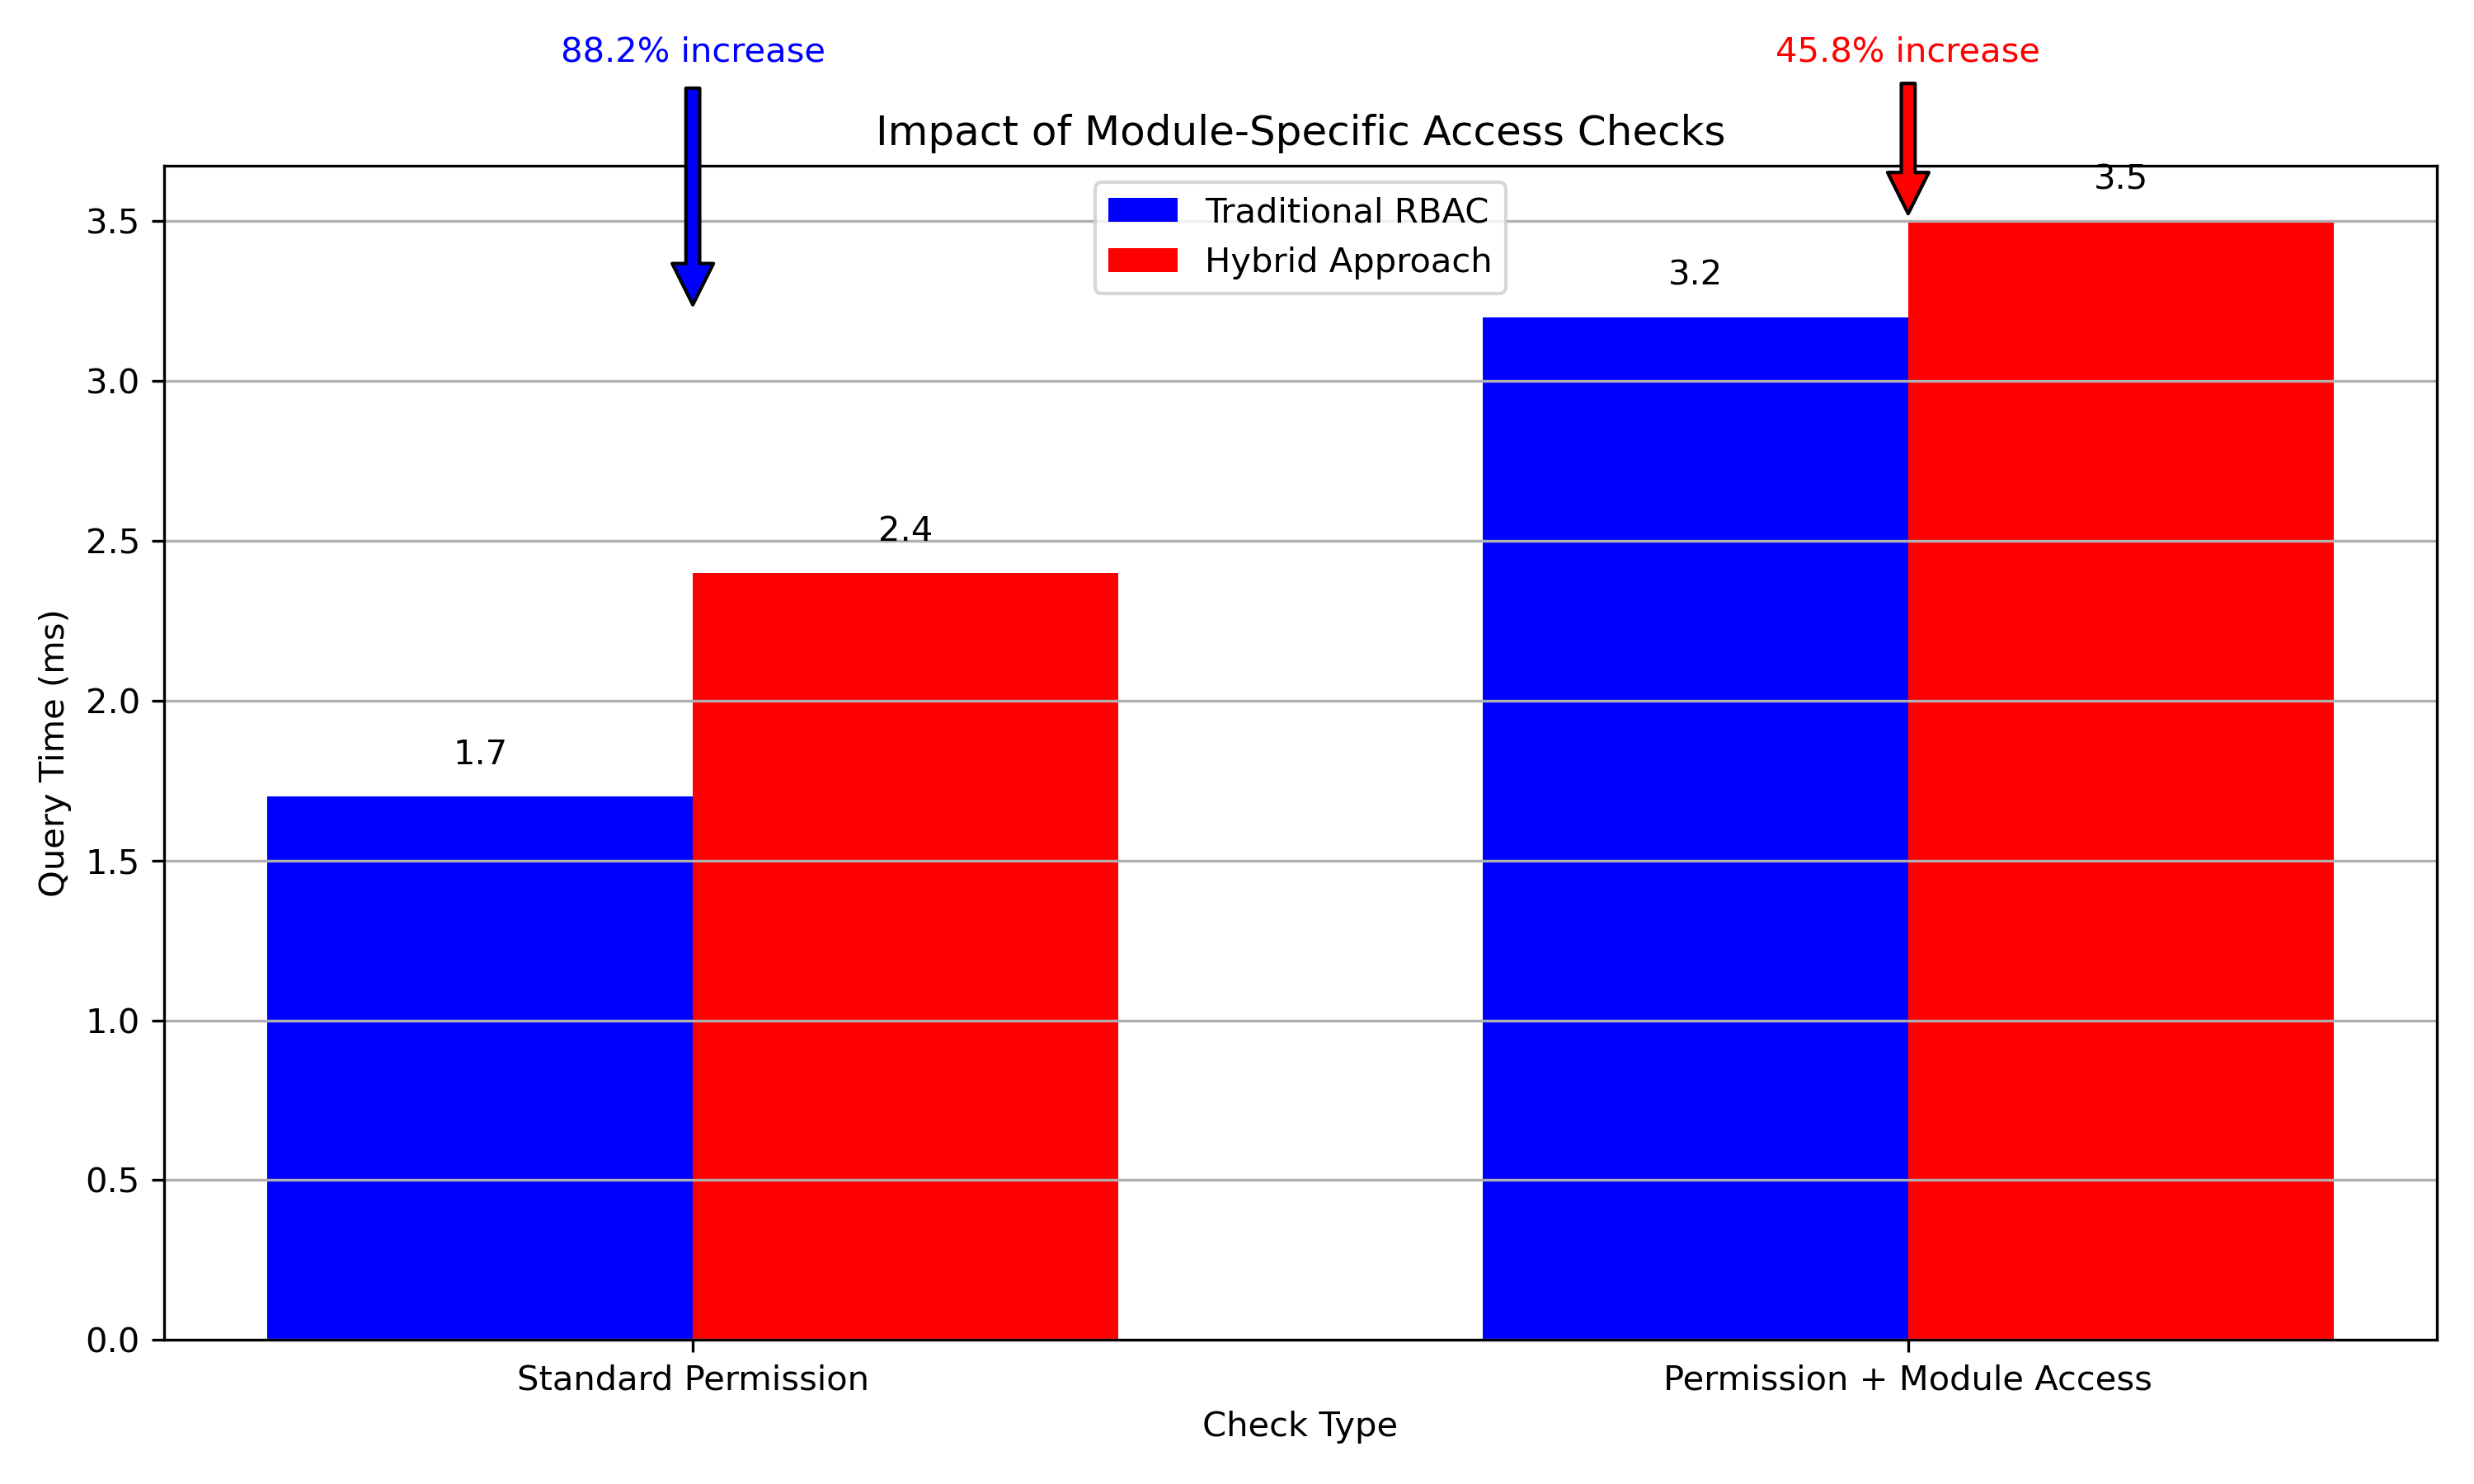
\includegraphics[width=0.8\textwidth]{figures/module_access_impact.png}
    \caption{Impact of Module-Specific Access Checks}
    \label{fig:module-access-impact}
\end{figure}

The performance analysis reveals that adding module-specific access verification introduces an 88.2\% overhead for the traditional role-based approach (increasing from 1.7ms to 3.2ms) and a 45.8\% overhead for the hybrid approach (increasing from 2.4ms to 3.5ms). Despite the performance overhead, both approaches maintain acceptable performance for interactive operations, with response times below 4ms for individual permission checks, confirming that the implemented module-specific access control provides the required access granularity without introducing prohibitive performance penalties.

\subsection{Release Management Validation}
\label{subsec:release-management-validation}

Release management testing evaluated the phase-based versioning approach that forms the foundation of the \ac{VMAP} system. Testing focused on four key aspects: phase sequence validation, phase transition operations, freeze functionality, and phase comparison. Phase sequence validation confirmed that the system correctly enforced the defined sequence of development phases with successful validation of each phase transition, essential for maintaining the structured development workflow described by Broy \cite{broy2006challenges} for automotive software development.

Phase transition testing verified that parameter configurations were correctly copied between phases with complete preservation of parameter-variant-segment relationships. Table \ref{tab:phase-transition-results} shows the test data revealing interesting patterns in development intensity across phases.

\begin{table}[h]
\centering
\caption{Phase Transition Test Results}
\label{tab:phase-transition-results}
\begin{tabular}{|l|c|c|p{2cm}|p{2cm}|c|}
\hline
\textbf{Transition Type} & \textbf{Variants} & \textbf{Segments} & \textbf{Added Variants} & \textbf{Added Segments} & \textbf{Time} \\
\hline
\multicolumn{6}{|c|}{\textbf{Baseline Dataset}} \\
\hline
Phase1 & 188 & 28,776 & - & - & - \\
\hline
Phase1 → Phase2 & 188 & 28,776 & 90 & 14,104 & 2.51s \\
\hline
Phase2 → Phase3 & 278 & 42,880 & 0 & 0 & 2.96s \\
\hline
Phase3 → Phase4 & 278 & 42,880 & 0 & 0 & 2.97s \\
\hline
\multicolumn{6}{|c|}{\textbf{Full Dataset}} \\
\hline
Phase1 & 830 & 167,990 & - & - & - \\
\hline
Phase1 → Phase2 & 830 & 167,990 & 170 & 41,113 & 12.39s \\
\hline
Phase2 → Phase3 & 1,000 & 209,103 & 0 & 0 & 12.87s \\
\hline
Phase3 → Phase4 & 1,000 & 209,103 & 0 & 0 & 12.89 \\
\hline
\end{tabular}
\end{table}

The test results reveal a significant pattern in development intensity across phases, consistent with Staron's observations \cite{staron2021automotive} regarding automotive software development cycles. The data demonstrates that the majority of parameter configurations occur during Phase1, with substantial additions in Phase2, while Phase3 and Phase4 typically involve refinement and validation rather than introducing new parameters or variants. This concentration of development activity in early phases aligns with the V-model approach common in automotive software development \cite{pretschner2007software}.

Phase transition performance characteristics showed only modest increases in execution time despite growing data volumes across phases. For the baseline dataset, transition times increased from 2.51s to approximately 3 seconds, demonstrating efficient scaling. Comparing baseline to full dataset transitions reveals transition times increasing to approximately 13 seconds, representing a sublinear scaling factor of approximately 4.3x for a dataset size increase of 5.6x.

Phase freezing functionality was validated through test cases targeting both database-level constraints and service-layer restrictions. The system successfully prevented modification attempts while maintaining appropriate read access, implementing the controlled milestone management required for regulated development environments as described by Staron \cite{staron2021automotive}.

\subsection{Variant Management Validation}
\label{subsec:variant-management-validation}

Variant management validation focused on assessing the system's capabilities for handling parameter customization through variants and segments. Testing employed an approach covering variant creation and segment modification workflows, using both the baseline dataset (188 variants, 28,776 segments) and the production-scale dataset (830 variants, 167,990 segments) to analyze functionality and performance under varying data volumes.

Variant creation testing verified proper implementation of domain constraints as defined in the conceptual architecture. Test cases included validation of unique name constraints within \acp{PID}, verification of proper code rule storage, and confirmation of correct relationship establishment between variants and their parent \acp{PID}. All test cases passed successfully for both scalar and complex parameters, with constraint enforcement consistently preventing invalid operations. As Vileikis \cite{vileikishacking} notes, constraint-based validation provides a robust foundation for maintaining data integrity in complex relational systems.

Performance analysis of variant operations revealed consistent response times across different variant complexities. Table \ref{tab:variant-operation-performance} details performance measurements for key variant operations under different data volumes.

\begin{table}[h]
\centering
\caption{Variant Operation Performance Metrics}
\label{tab:variant-operation-performance}
\begin{tabular}{|l|c|c|c|}
\hline
\textbf{Operation} & \textbf{Baseline Dataset} & \textbf{Production Dataset} & \textbf{Scaling Factor} \\
\hline
Variant Creation & 53ms & 55ms & 1.03x \\
\hline
Variant Update & 86ms & 124ms & 1.44x \\
\hline
Variant Retrieval & 45ms & 72ms & 1.60x \\
\hline
Variant Listing (per PID) & 38ms & 68ms & 1.79x \\
\hline
\end{tabular}
\end{table}

The observed scaling characteristics validate the effectiveness of the database schema design and indexing strategy described in Section \ref{sec:query-optimization}. The relatively small increase in execution time despite a 5x increase in data volume suggests efficient handling of larger datasets, with all operations remaining well under the 200ms threshold for interactive operations.

Segment modification testing employed a systematic approach covering one-dimensional arrays, two-dimensional matrices, and three-dimensional parameter representations. The database schema design proved effective for managing these complex data structures, with robust constraint enforcement correctly rejecting segment modifications with invalid dimension indices. Performance analysis for segment operations showed moderate scaling across different dataset sizes, with scaling factors ranging from 1.46x to 1.81x, validating the efficiency of the database schema design described in Section \ref{sec:entity-relationship-model}.

\section{Performance Analysis}
\label{sec:performance-analysis}

Beyond functional validation, performance analysis was conducted to assess the system's efficiency and scalability under various operational conditions. This section presents the key findings related to query performance and data volume scaling.

\subsection{Query Performance Assessment}
\label{subsec:query-performance-assessment}

Query performance was evaluated for common database operations across different data volumes. Figure~\ref{fig:query-performance-comparison} presents performance measurements for key query types between the baseline dataset (20,000 parameters) and full dataset (100,000 parameters).

\begin{figure}[h]
    \centering
    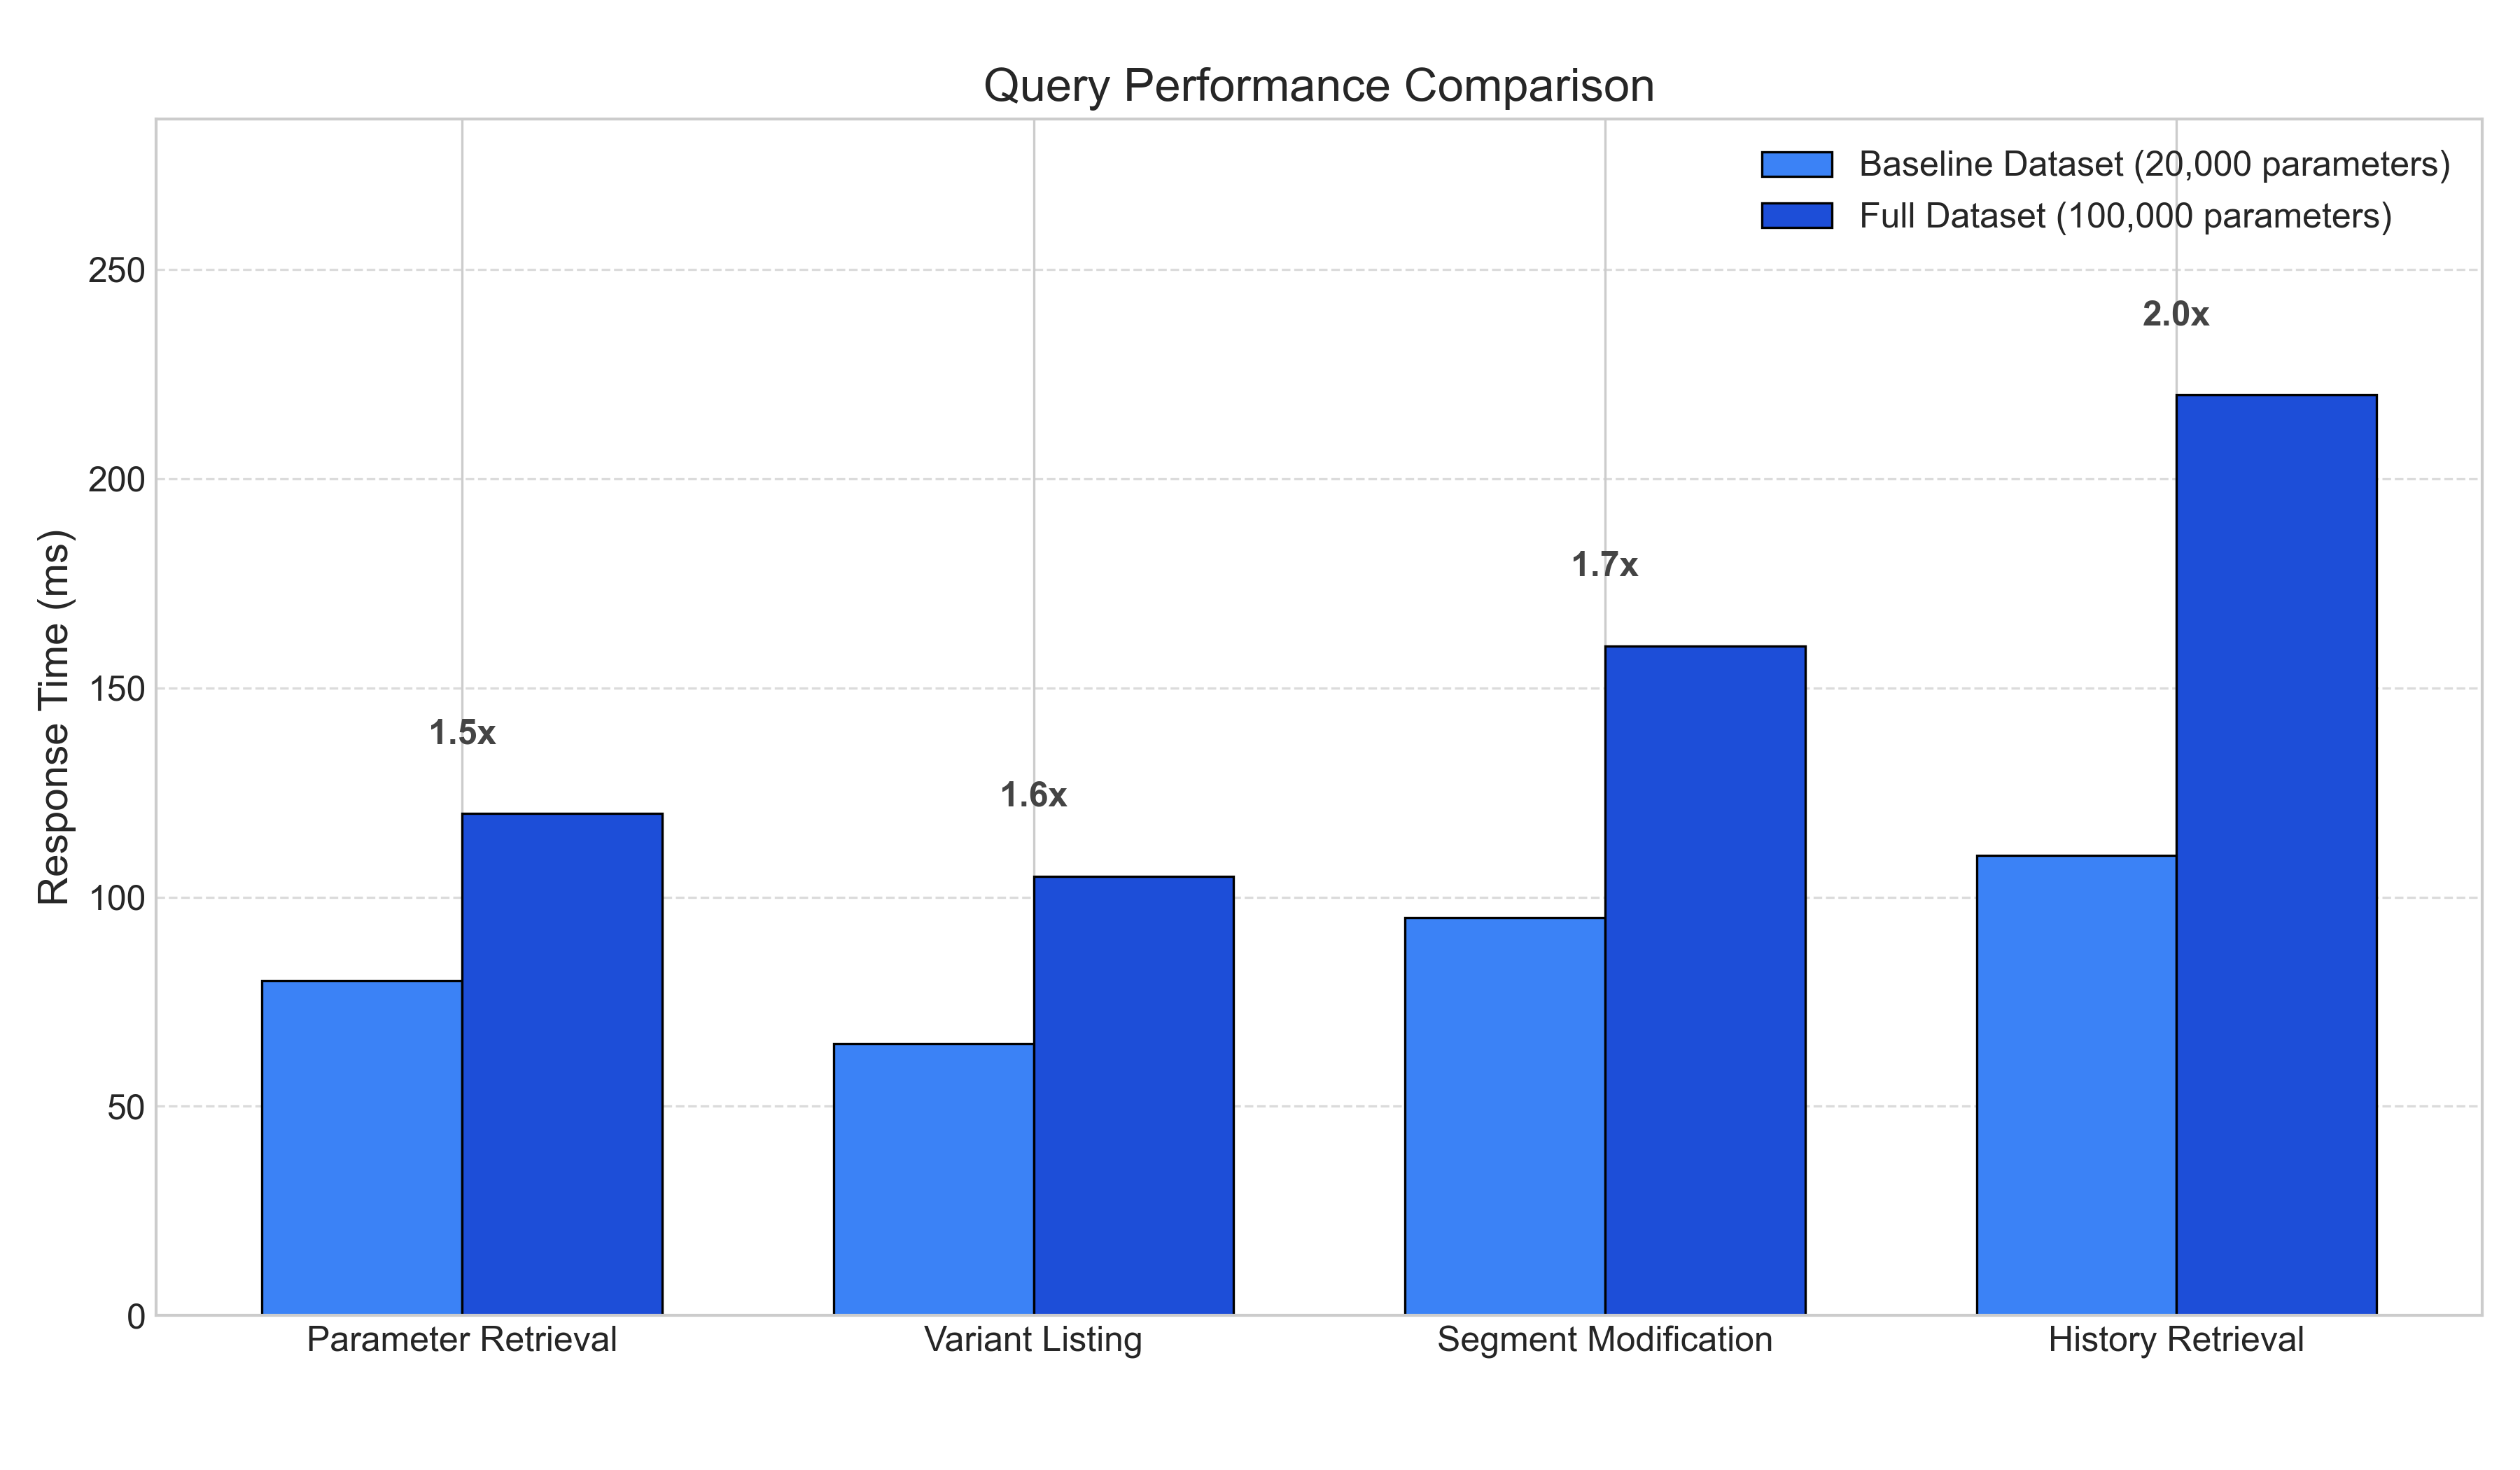
\includegraphics[width=0.8\textwidth]{figures/query_performance_comparison.png}
    \caption{Query Performance Comparison}
    \label{fig:query-performance-comparison}
\end{figure}

The performance analysis reveals that most common operations maintain reasonable performance with increasing data volumes. The system maintained interactive response times (below 200ms) for most operations even with the full dataset, ensuring a responsive user experience. Parameter retrieval operations showed a scaling factor of 1.5x when moving from the baseline to full dataset, while variant listing demonstrated a slightly higher factor of 1.6x. History retrieval operations exhibited the highest scaling factor among standard queries at 2.0x, reflecting the additional processing required when retrieving records from the substantially larger audit history tables.

The phase comparison operation demonstrated longer execution times and suboptimal scaling, with execution times increasing from 2.8s for the baseline dataset to 12.4s for the full dataset—a scaling factor of 4.4x. This operation exceeds the interactive response threshold for larger datasets, identifying it as a candidate for future optimization. The execution of queries with and without indexes demonstrated the critical importance of the indexing strategy, with response times increasing by factors of 6.5x to 21.8x without proper indexes.

\subsection{Indexing Strategy Performance Validation}
\label{subsec:indexing-strategy-performance}

The indexing strategy described in Section \ref{sec:query-optimization} was validated through comprehensive performance measurements comparing query execution times with and without strategic indexes. Figure \ref{fig:index-performance-comparison} presents the performance comparison across five critical query patterns that represent the dominant access patterns in automotive parameter management workflows.

\begin{figure}[h]
    \centering
    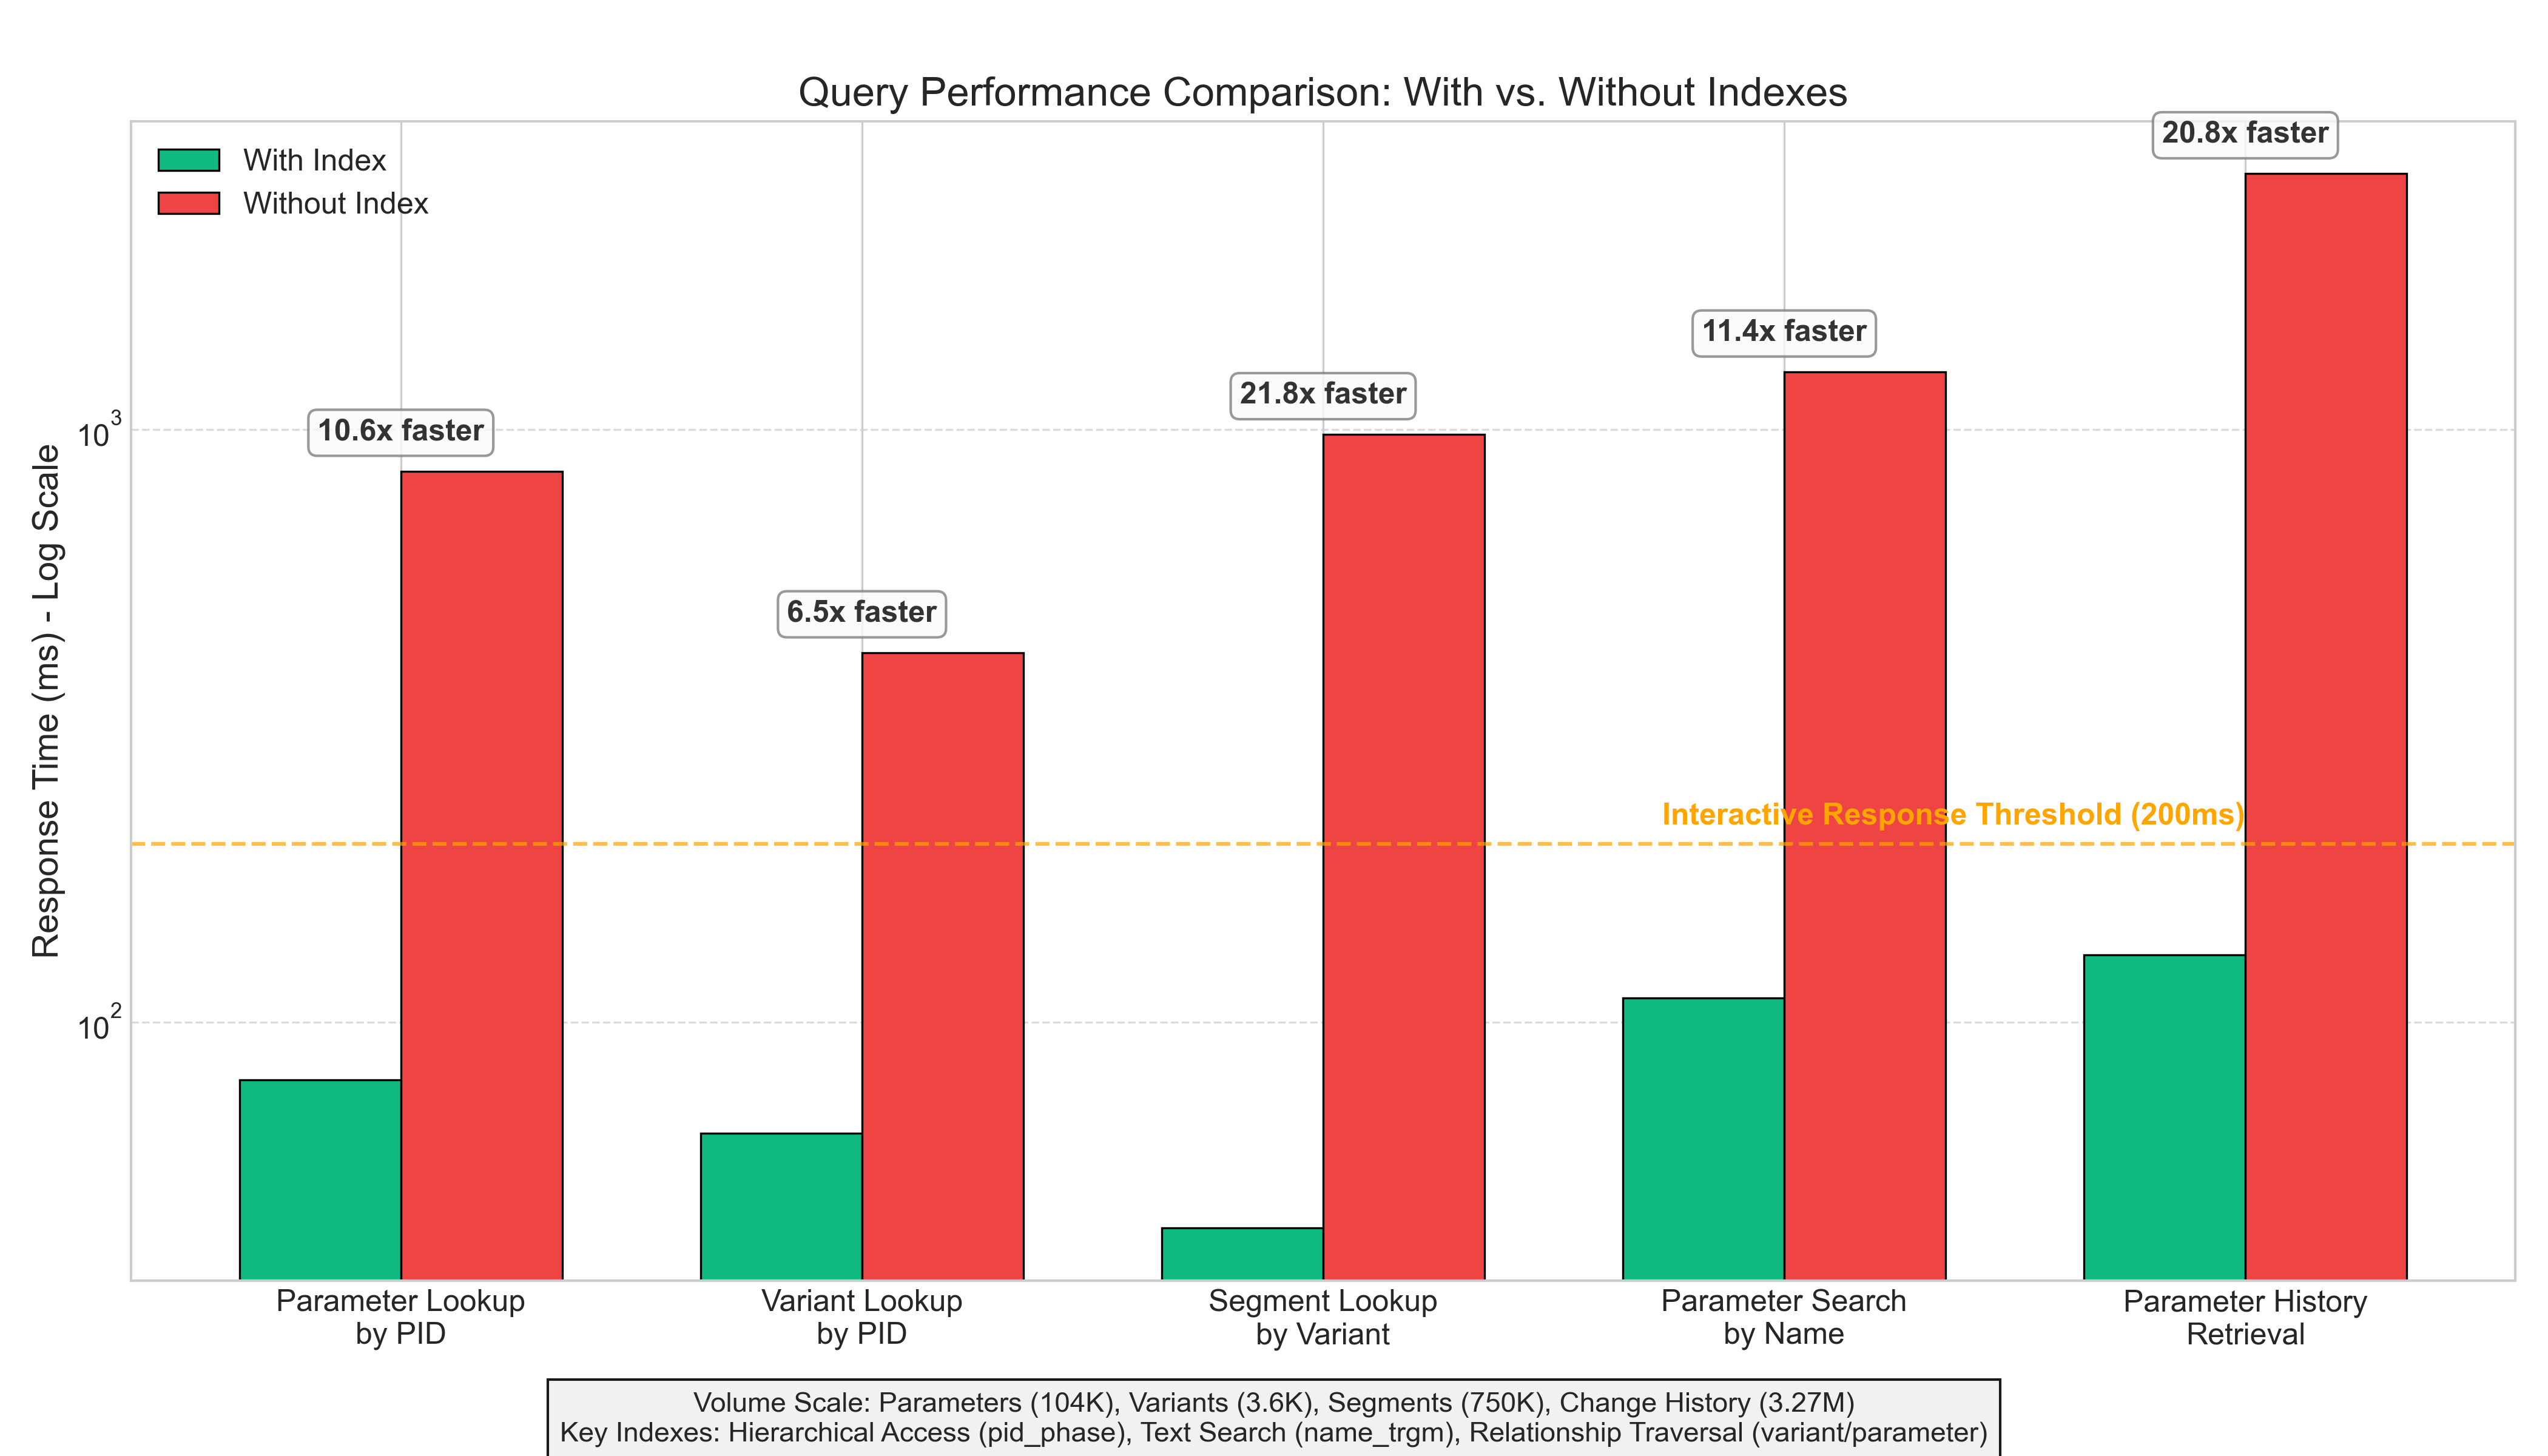
\includegraphics[width=0.95\textwidth]{figures/index_performance_comparison.png}
    \caption{Query Performance Comparison: With vs. Without Indexes}
    \label{fig:index-performance-comparison}
\end{figure}

The performance evaluation demonstrates the critical importance of the implemented indexing strategy for maintaining interactive response times in production environments. Parameter lookup operations by PID achieved a 10.6x performance improvement, reducing response times from 850ms to 80ms through the \texttt{idx\_parameters\_\allowbreak pid\_\allowbreak phase} composite index. Variant lookup operations showed a 6.5x improvement, with response times decreasing from 420ms to 65ms using the same hierarchical indexing approach. The most dramatic improvement was observed in segment lookup operations, which achieved a 21.8x speedup from 980ms to 45ms through the \texttt{idx\_segments\_variant} index, reflecting the efficiency of direct relationship traversal compared to sequential scanning.

Text-based parameter search operations, enabled by PostgreSQL's trigram indexes, demonstrated an 11.4x performance improvement from 1,250ms to 110ms. This capability is particularly valuable for engineering workflows where parameters are often located through partial name matching rather than exact hierarchical navigation. Parameter history retrieval, which accesses the extensive change history tables containing over 3.2 million records, showed the most substantial absolute improvement with a 20.8x speedup from 2,700ms to 130ms, validating the effectiveness of the audit system indexing strategy described in Section \ref{sec:audit-system}.

All indexed operations maintained response times well below the 200ms interactive response threshold, ensuring that the system provides a responsive user experience even with production-scale datasets containing over 100,000 parameters. The performance improvements validate the strategic indexing decisions made during implementation, particularly the use of composite indexes for hierarchical navigation and specialized trigram indexes for text-based searching. These results demonstrate that the database design successfully addresses the performance requirements of automotive parameter management while maintaining the comprehensive audit capabilities essential for regulatory compliance.

\subsection{Variant Operation Performance}
\label{subsec:variant-operation-performance}

Variant operation performance was assessed across different data volumes to evaluate the system's handling of core parameter customization workflows. Figure~\ref{fig:variant-performance} illustrates the performance of variant operations under different data volumes.

\begin{figure}[h]
    \centering
    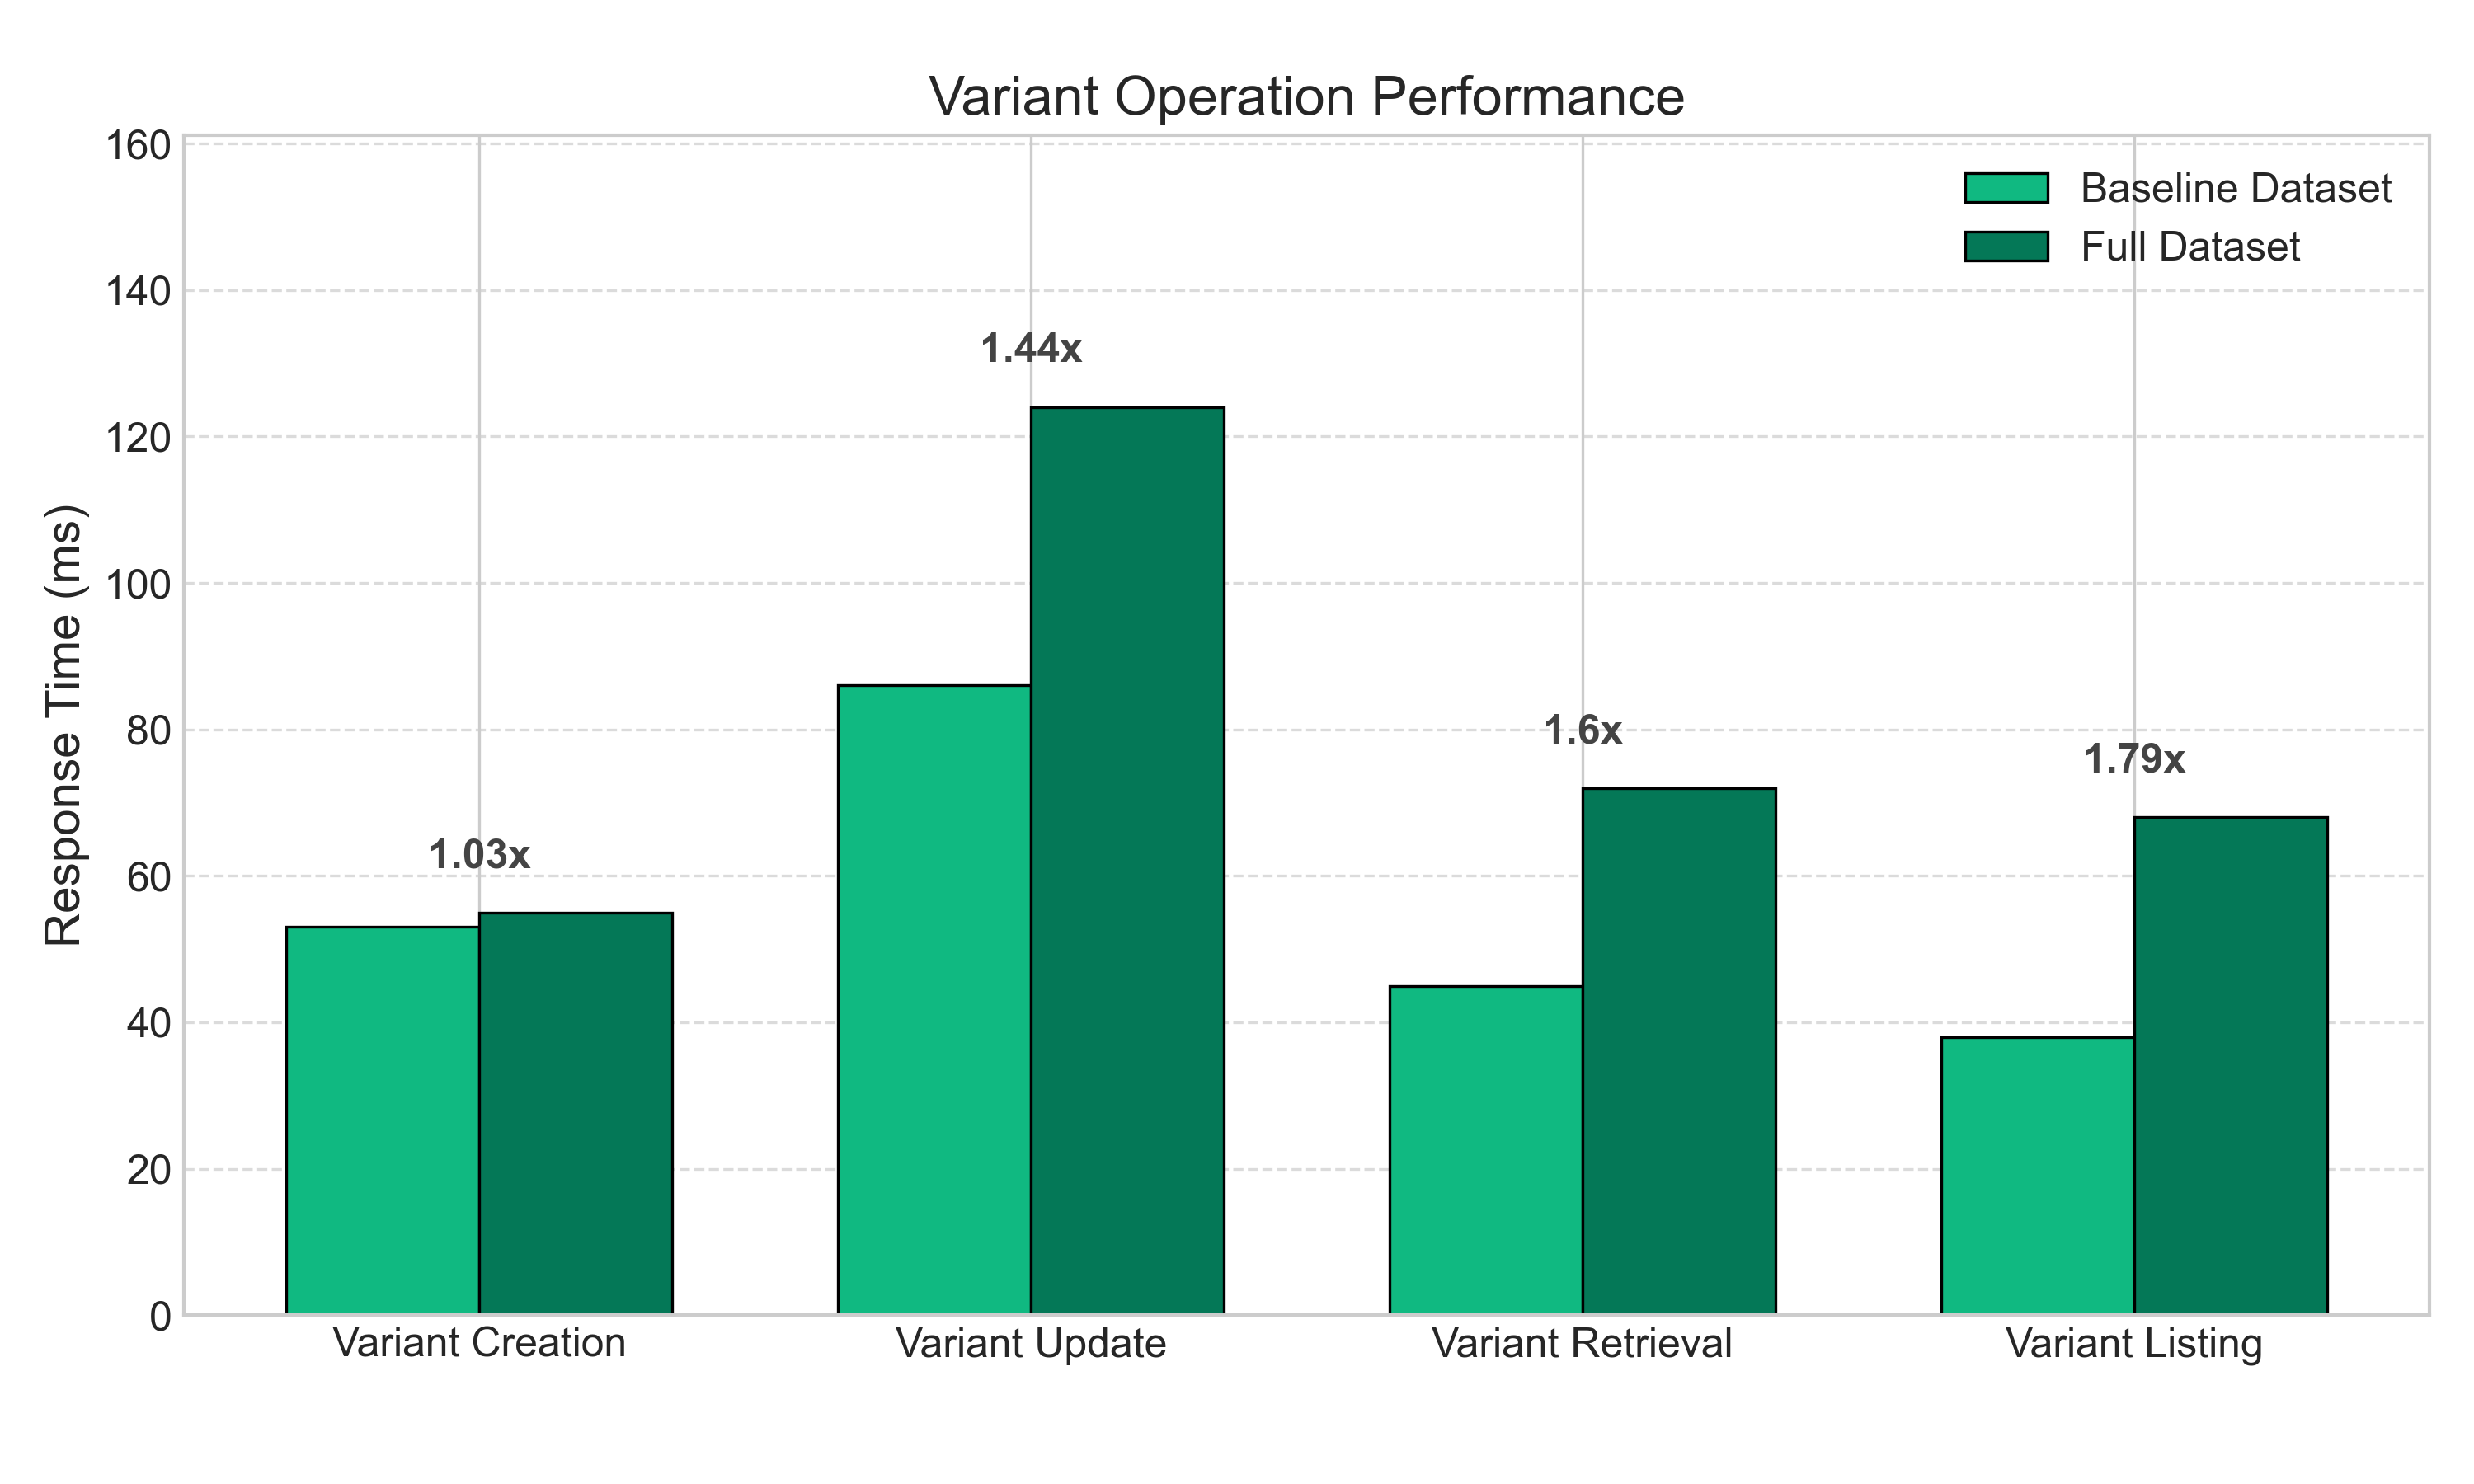
\includegraphics[width=0.8\textwidth]{figures/variant_performance.png}
    \caption{Variant Operation Performance}
    \label{fig:variant-performance}
\end{figure}

The analysis reveals consistent response times across different operation types, with scaling factors ranging from 1.03x for variant creation to 1.79x for variant listing when comparing baseline and full datasets. Variant creation operations demonstrated excellent scaling characteristics (1.03x), showing minimal performance impact despite the five-fold increase in dataset size. This efficiency can be attributed to the well-designed primary key and constraint implementation, allowing new records to be inserted with minimal overhead regardless of existing data volume. The average scaling factor across all variant operations was approximately 1.47x, indicating that these operations scale efficiently with increasing data volumes, with all variant operations maintaining response times under 125ms for the full dataset.

\subsection{Storage Requirements Analysis}
\label{subsec:storage-requirements-analysis}

Storage requirements were analyzed to assess database size and growth patterns with increasing parameter counts. Figure~\ref{fig:storage-analysis} presents the storage allocation across different entity types for the full dataset.

\begin{figure}[h]
    \centering
    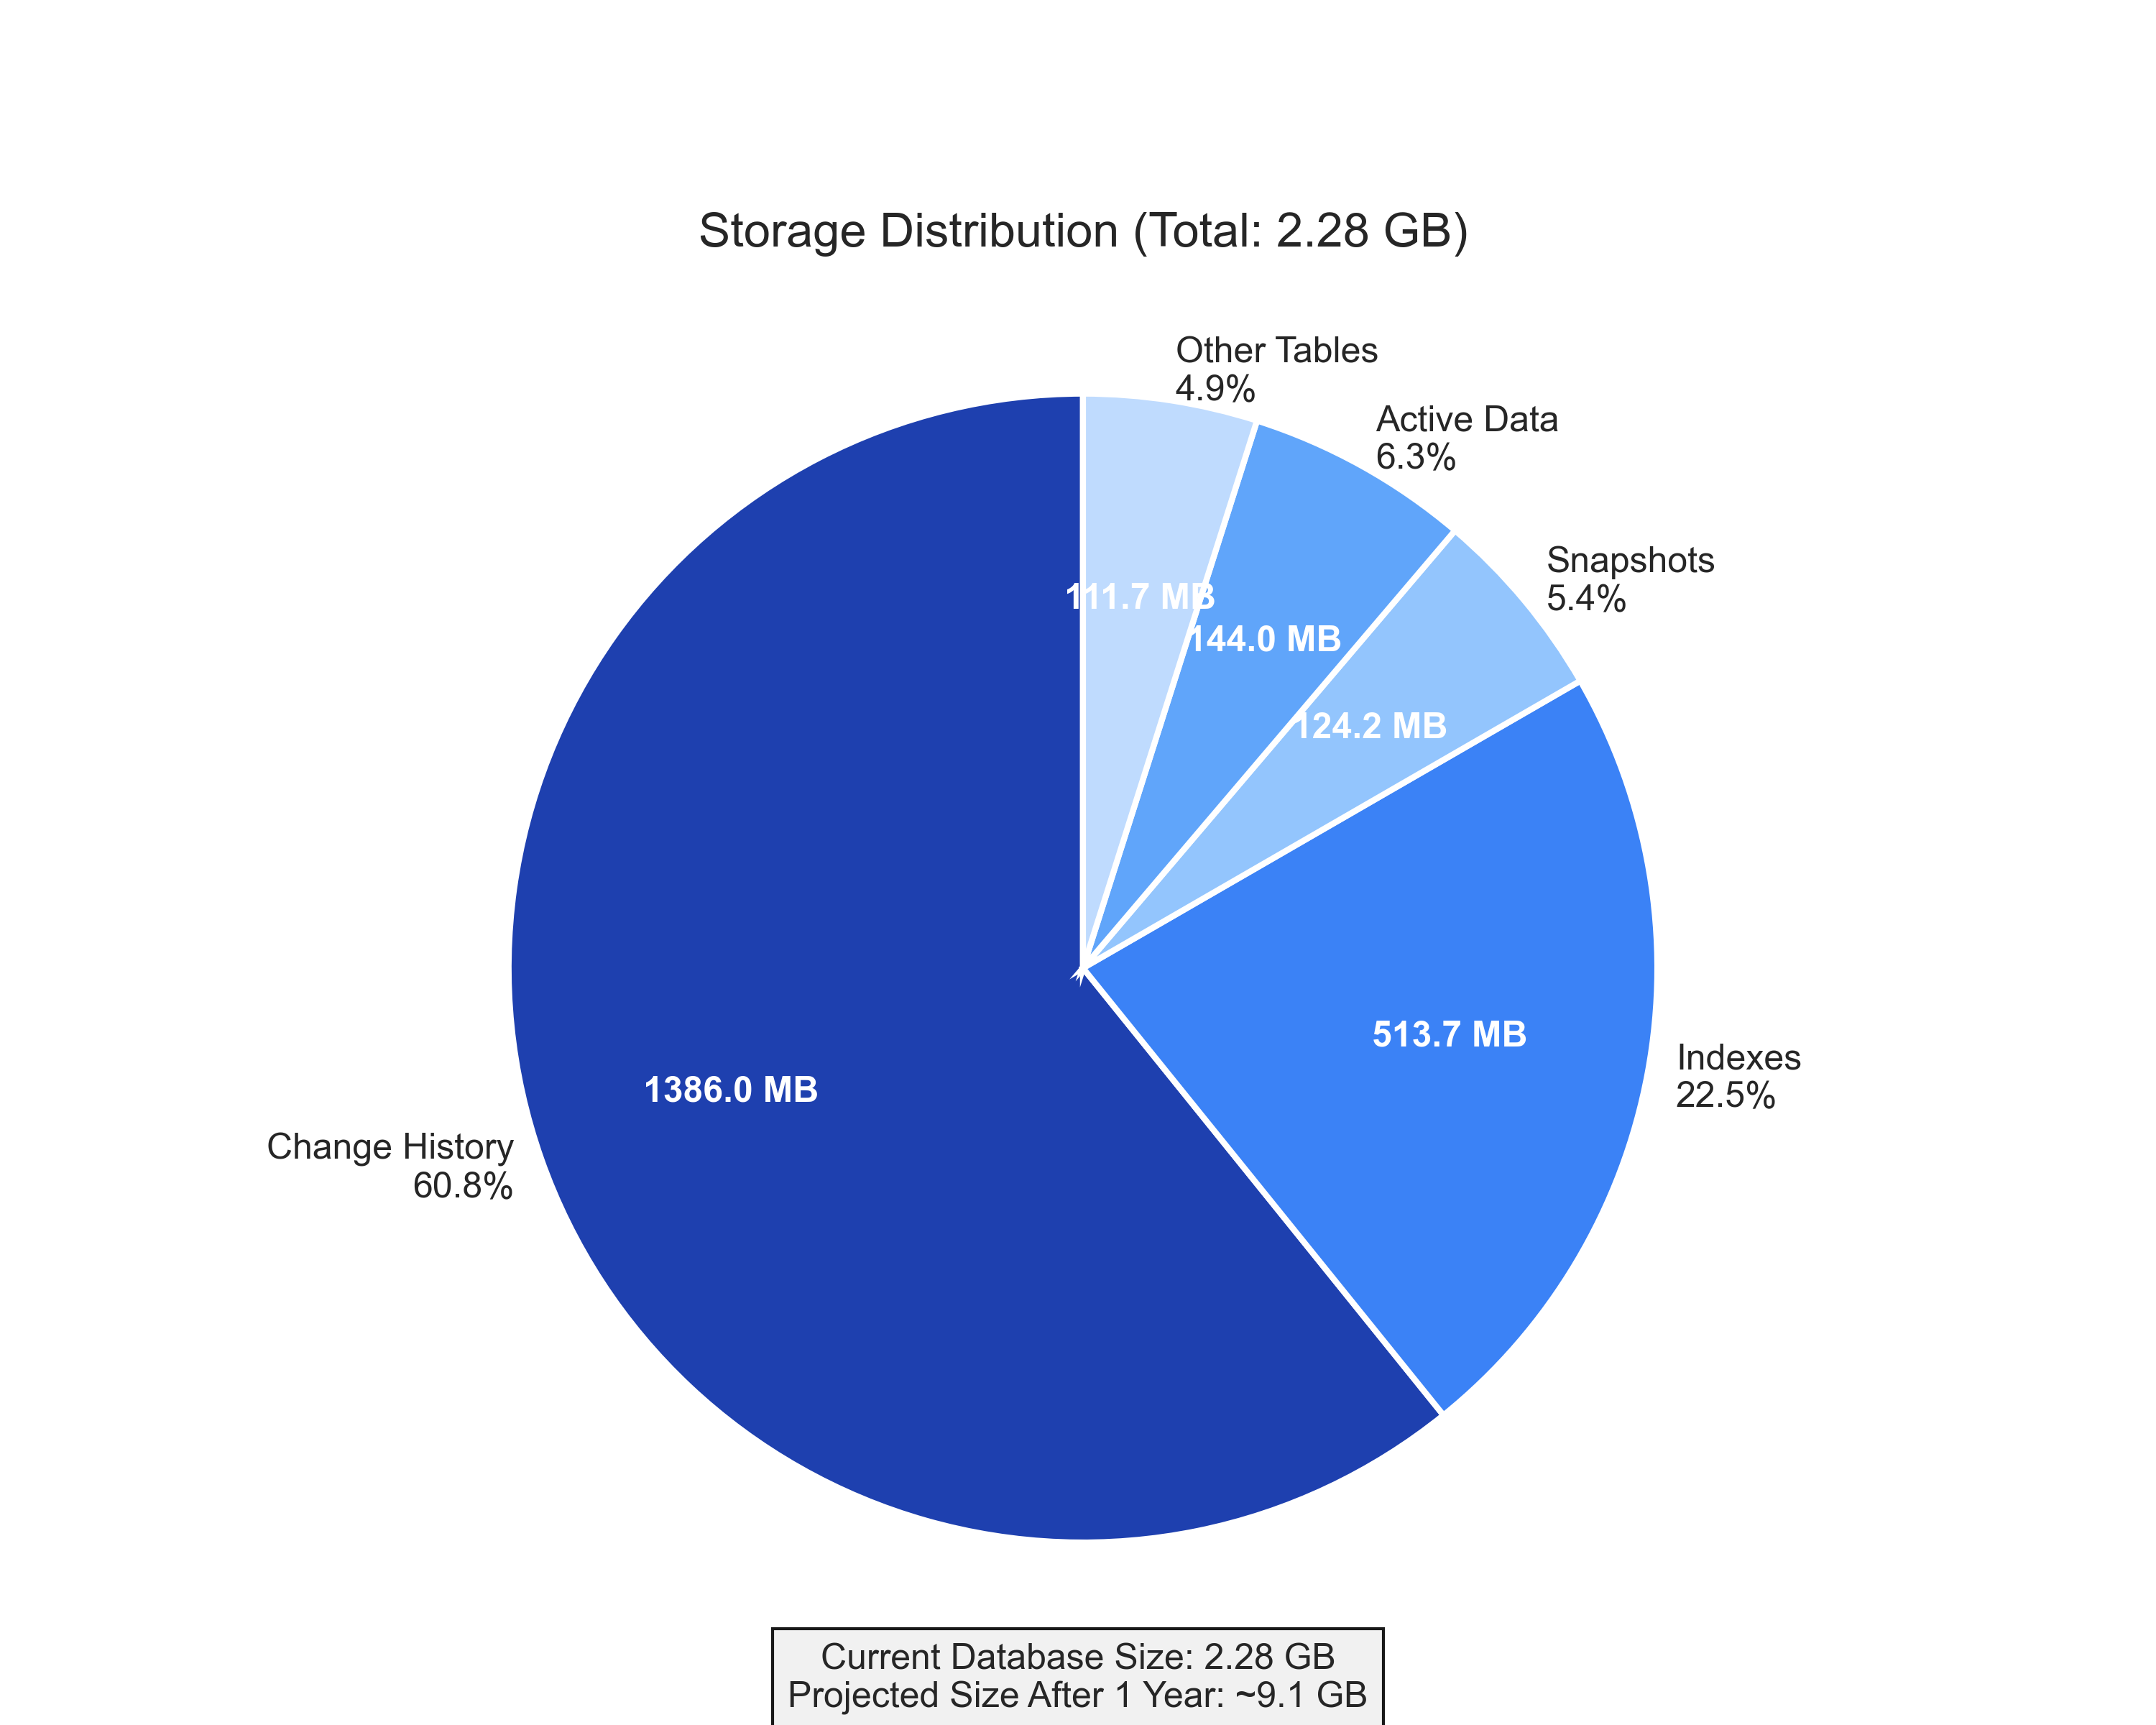
\includegraphics[width=0.8\textwidth]{figures/storage_distribution.png}
    \caption{Storage Distribution by Entity Type}
    \label{fig:storage-analysis}
\end{figure}

The analysis reveals that the change history table dominates the database storage allocation, accounting for approximately 60.8\% of the total database size. This distribution significantly exceeds the storage requirements of the current data state, aligning with Bhattacherjee's observations~\cite{bhattacherjee2015principles} regarding versioning and audit systems. While there are only 3,617 variants in the current state, the system maintains over 3.2 million change history records, reflecting the comprehensive auditing approach implemented in the system.

\begin{table}[h]
\centering
\caption{Storage Requirements Analysis}
\label{tab:storage-requirements}
\begin{tabular}{|l|r|r|}
\hline
\textbf{Entity Type} & \textbf{Record Count} & \textbf{Storage Size (MB)} \\
\hline
Parameters & 104,428 & 43.0 \\
\hline
Variants & 3,617 & 1.0 \\
\hline
Segments & 750,009 & 100.0 \\
\hline
Change History & 3,270,511 & 1,386.0 \\
\hline
Documentation Snapshots & 7 & 0.1 \\
\hline
Snapshot Variants & 4,980 & 0.1 \\
\hline
Snapshot Segments & 1,007,940 & 124.0 \\
\hline
Other Tables & - & 111.7 \\
\hline
Indexes & - & 513.7 \\
\hline
\textbf{Total} & - & \textbf{2,279.6} \\
\hline
\end{tabular}
\end{table}

Despite having only 7 documentation snapshots, the system maintains over 1 million snapshot segments, exceeding the count of active segments. This indicates that documentation snapshots capture extensive parameter configurations at specific time points, creating substantial storage requirements for historical state preservation. The index structures consume approximately 22.5\% of the total storage, reflecting the sophisticated indexing strategy described in Section~\ref{sec:query-optimization}. While this represents significant overhead, it provides essential performance benefits for query operations.

The actual active data—parameters, variants, and segments—consumes only 6.3\% of the total database size, with the majority of storage dedicated to audit trails, snapshots, and indexes. This distribution aligns with the requirements for regulated development environments described by Staron~\cite{staron2021automotive}, where comprehensive traceability and historical record maintenance are essential for compliance and quality assurance.

\subsection{Versioning Approach Performance}
\label{subsec:versioning-approach-performance}

The performance characteristics of the phase-based parameter versioning approach selected in Chapter~\ref{chap:methodology} were evaluated against the alternative change-based approach. Figure~\ref{fig:versioning-approach-comparison} presents the performance comparison between the two approaches for parameter retrieval operations across different data volumes, along with the storage requirements for each approach.

\begin{figure}[h]
    \centering
    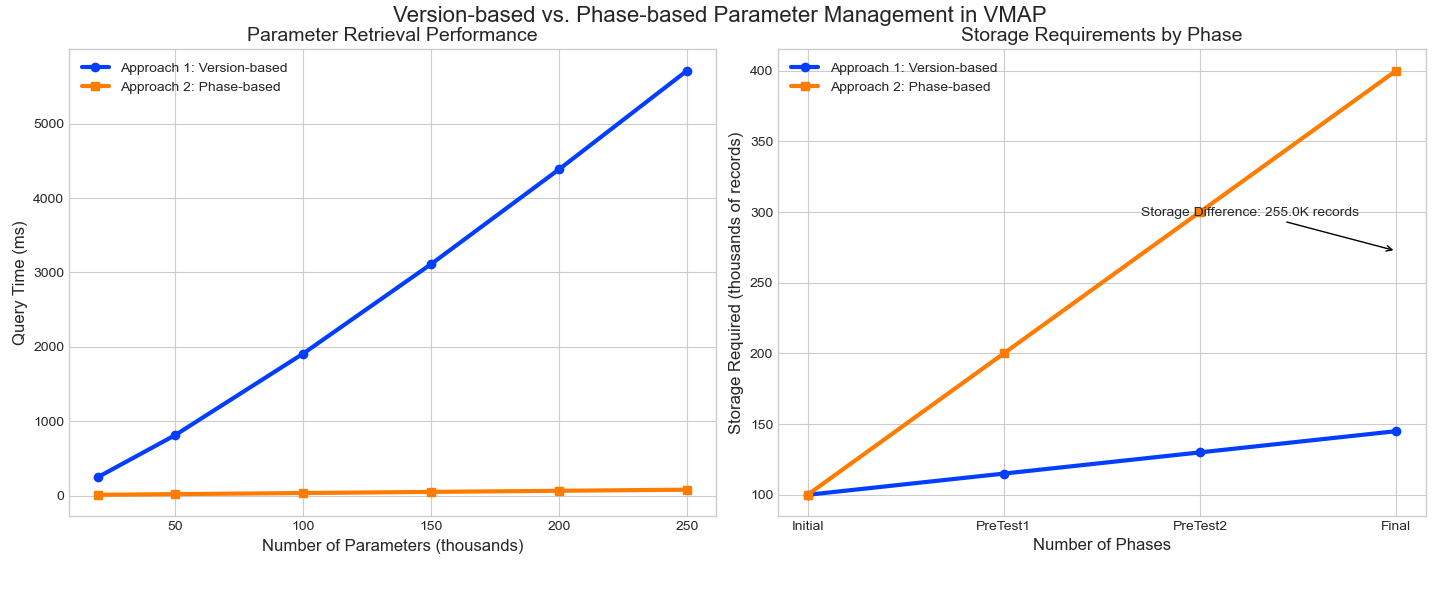
\includegraphics[width=0.8\textwidth]{figures/vmap_versioning_approaches_simplified.png}
    \caption{Version-based vs. Phase-based Parameter Management Comparison}
    \label{fig:versioning-approach-comparison}
\end{figure}

The performance analysis demonstrates that the phase-based approach offers better query performance, particularly as parameter counts increase. For the tested parameter counts, the phase-based approach remains below 100ms for parameter retrieval operations, while the version-based approach shows nonlinear growth with increasing parameter counts. The storage requirements analysis confirms that the phase-based approach consumes approximately 51\% higher storage requirements across all phases. However, this storage difference represents a reasonable tradeoff given the performance benefits for query operations, as noted by Bhattacherjee et al.~\cite{bhattacherjee2015principles}.

These findings validate the architectural decision to implement a phase-based versioning approach for the \ac{VMAP} system. While consuming more storage than a version-based approach, the phase model provides performance benefits, implementation simplicity, and alignment with domain concepts that outweigh the additional storage requirements.

\section{Integration Testing}
\label{sec:integration-testing}

Integration testing evaluated the system's interaction with external enterprise systems, focusing on Parameter Definition Database synchronization and Vehicle Configuration Database integration.

\subsection{Parameter Definition Database Synchronization}
\label{subsec:pdd-synchronization-testing}

Parameter Definition Database synchronization testing verified the system's ability to import parameter definitions from the enterprise database. Figure \ref{fig:pdd-sync-time} illustrates the synchronization time trends observed during testing.

\begin{figure}[h]
    \centering
    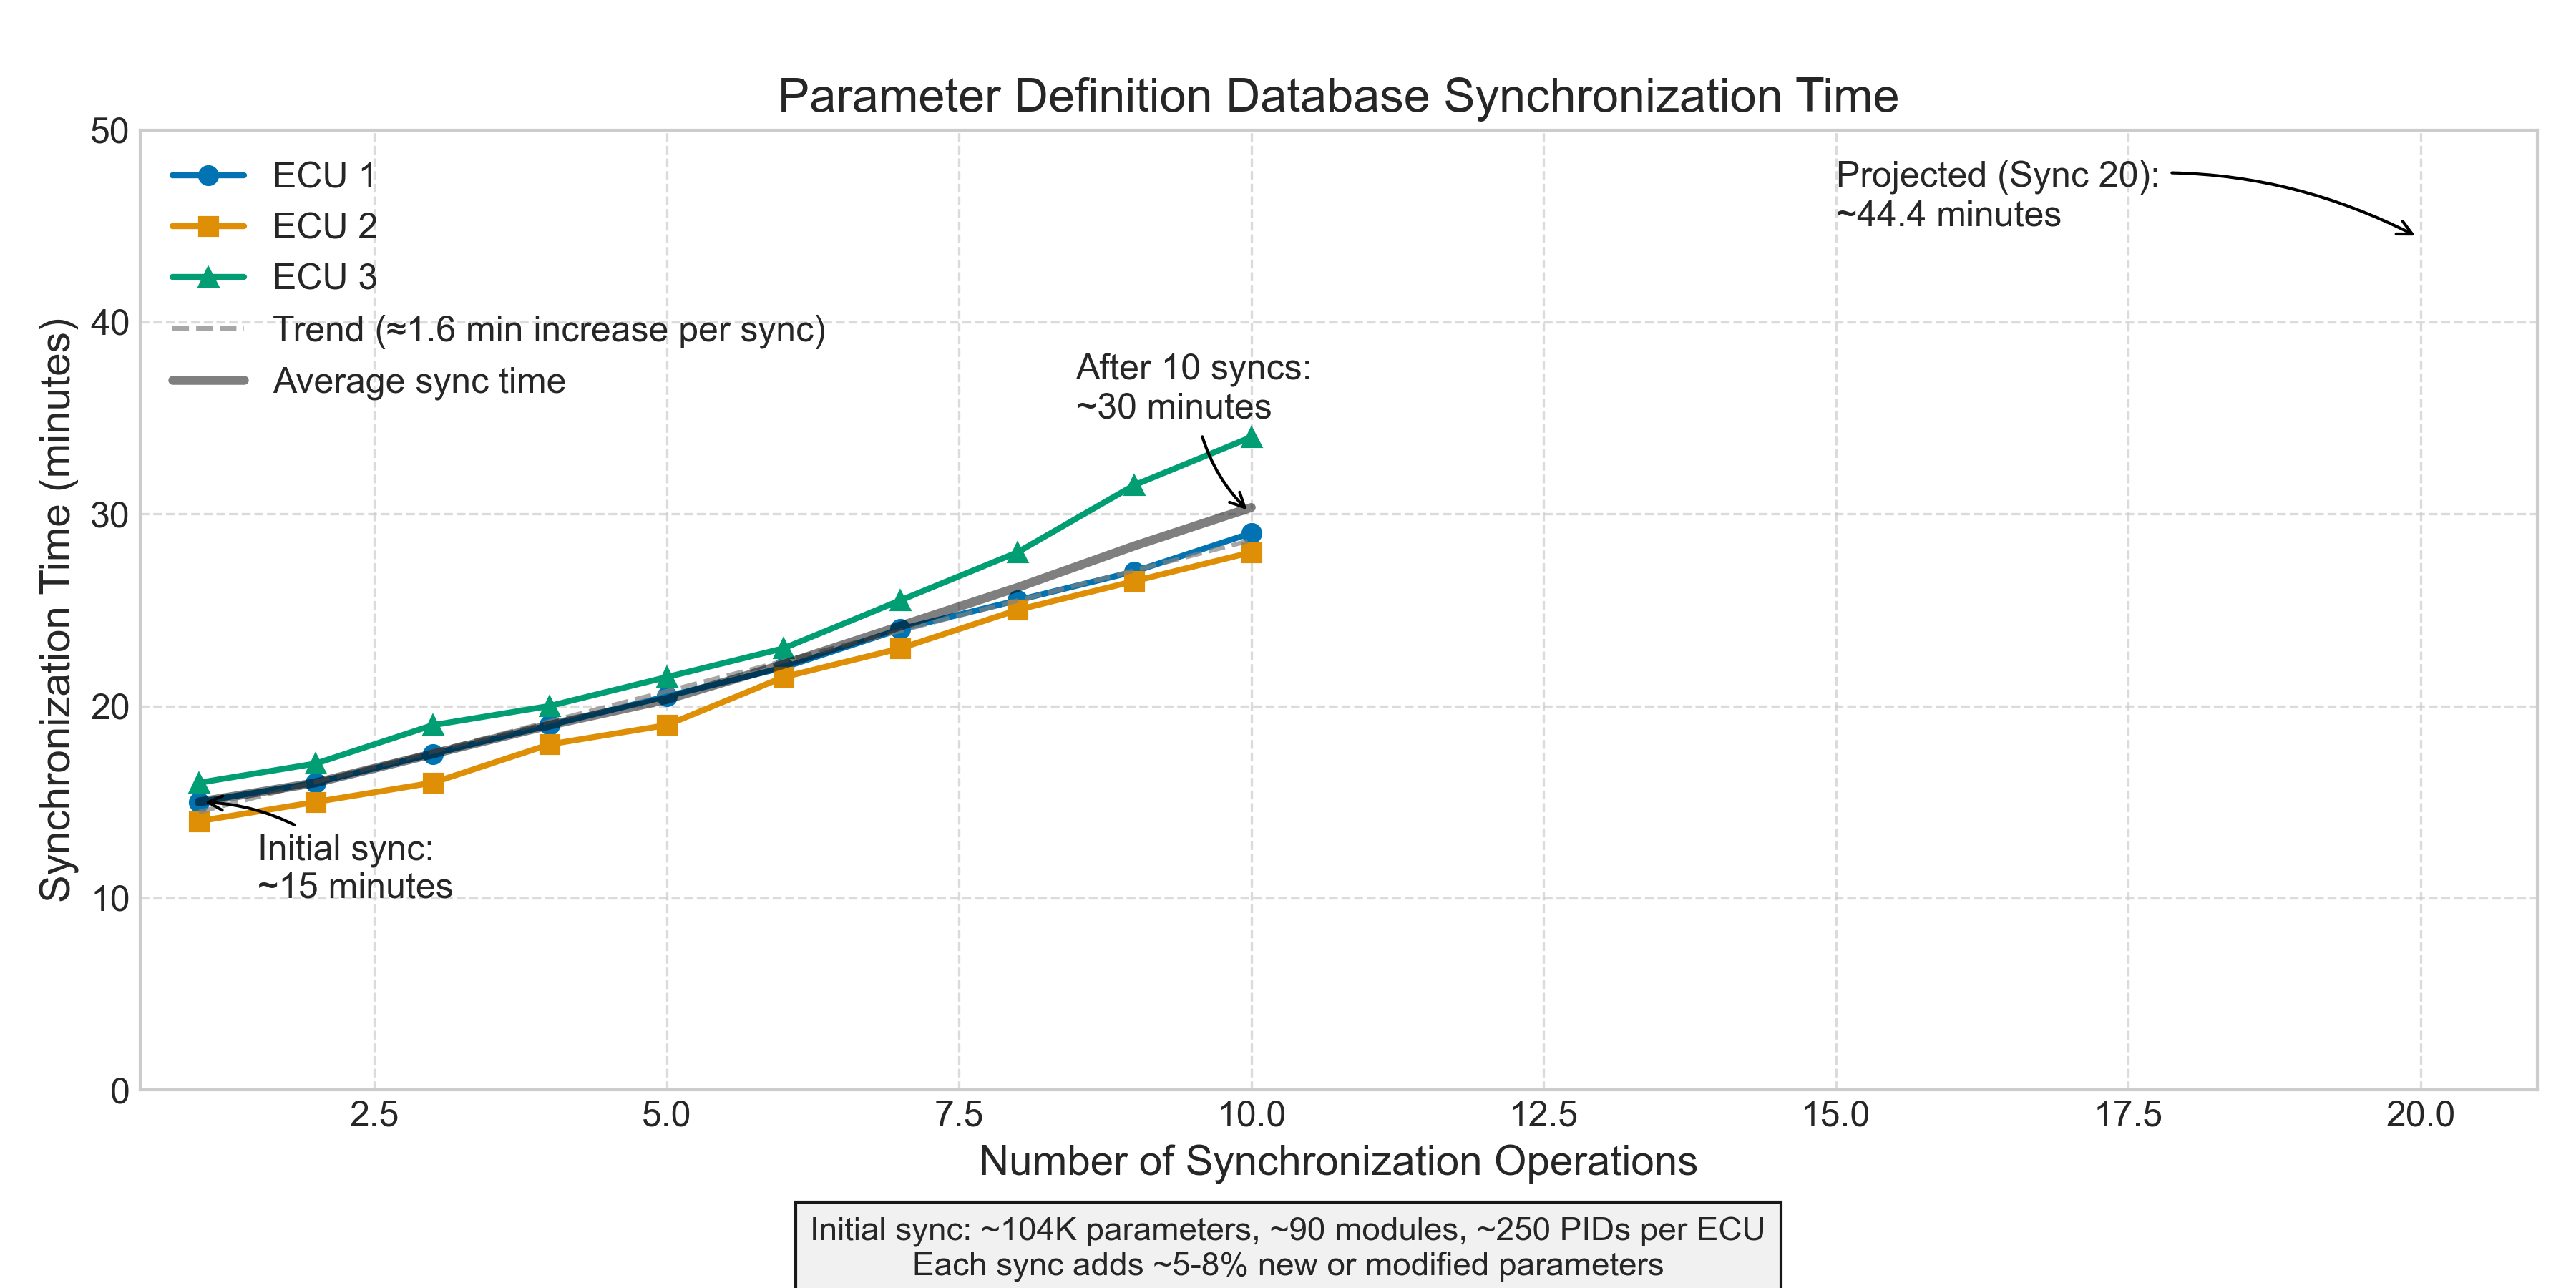
\includegraphics[width=0.8\textwidth]{figures/pdd_sync_time_graph.png}
    \caption{Parameter Definition Database Synchronization Time Trends}
    \label{fig:pdd-sync-time}
\end{figure}

The synchronization performance analysis revealed an increasing trend in execution time over successive synchronization operations. Initial synchronization operations required approximately 15 minutes for the tested \acp{ECU}, with execution times increasing to around 30 minutes after 10 synchronization cycles. This gradual increase aligns with the observations of Mueller and Müller \cite{mueller2018conception} regarding database synchronization in complex engineering environments.

Table \ref{tab:pdd-sync-results} presents the success rates for different types of parameter changes during synchronization operations.

\begin{table}[h]
\centering
\caption{Parameter Definition Database Synchronization Results}
\label{tab:pdd-sync-results}
\begin{tabular}{|l|c|c|c|}
\hline
\textbf{Change Type} & \textbf{Processed} & \textbf{Succeeded} & \textbf{Success Rate} \\
\hline
New Parameters & 5,218 & 5,218 & 100\% \\
\hline
Modified Parameters & 3,764 & 3,691 & 98.1\% \\
\hline
New Modules & 12 & 12 & 100\% \\
\hline
New \acp{PID} & 67 & 67 & 100\% \\
\hline
Removed Parameters & 42 & 42 & 100\% \\
\hline
\end{tabular}
\end{table}

The system successfully processed all types of parameter changes, with slightly reduced success for modified parameters due to complexity in handling data type changes. Based on the observed synchronization performance trends, the projected synchronization time for the 20th cycle would reach approximately 45 minutes. While still acceptable for the typical synchronization frequency, this suggests that synchronization performance optimization would be beneficial for long-term system maintenance.

Vehicle Configuration Database integration testing verified the system's ability to use vehicle configuration data for code rule evaluation and parameter file generation. Vehicle configuration data import testing confirmed that the system could correctly import and store vehicle configuration codes, with proper mapping between codes and vehicles. Code rule validation testing verified that the system could evaluate boolean expressions against vehicle configurations, with the evaluation engine correctly interpreting both simple logical operators and complex nested expressions. Parameter file generation testing confirmed that the system could produce valid parameter files for vehicle testing, with correct application of variant selection logic based on vehicle configuration codes.

\section{Feature Comparison with Excel-Based Approach}
\label{sec:feature-comparison-excel}

To assess the improvements provided by the \ac{VMAP} system, a feature comparison was conducted against the Excel-based approach currently used for parameter management. Table \ref{tab:feature-comparison} presents a comparison of key features between the \ac{VMAP} system and the Excel-based approach.

\begin{table}[h]
\centering
\caption{Feature Comparison with Excel-Based Approach}
\label{tab:feature-comparison}
\begin{tabular}{|l|c|c|}
\hline
\textbf{Feature} & \textbf{VMAP Database} & \textbf{Excel Approach} \\
\hline
Variant Management & Comprehensive & Limited \\
\hline
Multi-User Support & Concurrent & Sequential \\
\hline
Change Tracking & Automatic & Manual \\
\hline
Version Control & Phase-Based & File-Based \\
\hline
Access Control & Role + Module & File Permission \\
\hline
Validation & Automatic & Manual \\
\hline
Documentation & Integrated & Separate \\
\hline
Integration & Automated & Manual \\
\hline
\end{tabular}
\end{table}

The \ac{VMAP} system provides significant advantages in all feature categories, with particular improvements in multi-user support, change tracking, and access control. The \ac{VMAP} system demonstrated superior data integrity protection, correctly preventing invalid operations through database constraints and business rule validation. The database-level constraints and validation mechanisms provide a robust defense against data corruption, implementing the comprehensive validation approach described in Section \ref{sec:validation-mechanisms}.

Beyond technical improvements, the \ac{VMAP} system introduces significant enhancements to the automotive parameter development process. The centralized database approach enables concurrent work by multiple engineers, eliminating the file sharing bottlenecks common in the Excel-based approach. The role-based access control ensures that engineers can modify only their assigned modules, preventing accidental changes to other areas. The phase-based versioning approach aligns naturally with the automotive development lifecycle, supporting the structured progression from initial development through testing to final release. The comprehensive change tracking and documentation features address regulatory compliance requirements, providing complete traceability for all parameter modifications, increasingly important in the context of functional safety standards like ISO 26262.
    \cleardoublepage
    \chapter{Conclusion and Future Work}
\label{chap:conclusion}

This thesis presented the design, implementation, and evaluation of the \ac{VMAP} database system for automotive parameter management. The research addressed critical challenges in parameter versioning, access control, and enterprise integration through a comprehensive PostgreSQL-based solution that replaces error-prone spreadsheet approaches with structured database management.

\section{Research Contributions}
\label{sec:research-contributions}

The \ac{VMAP} system delivers significant advancements in automotive parameter management through four key contributions that address fundamental limitations in current approaches.

The phase-based versioning model provides an effective alternative to generic temporal database approaches by aligning parameter evolution with automotive development cycles. Unlike traditional change-based versioning, this domain-specific strategy supports simultaneous work across development phases while maintaining milestone integrity and clear separation between development stages. The approach enables efficient parameter retrieval without complex reconstruction while supporting the structured progression common in automotive engineering.

The hybrid role-permission access control model combines traditional \ac{RBAC} with module-specific permissions to accommodate complex organizational structures in automotive development. This approach balances administrative simplicity with access granularity, supporting engineers who typically have responsibility for specific vehicle subsystems rather than entire parameter sets. Comprehensive constraint enforcement maintains security while providing the flexibility needed for specialized access patterns.

The enterprise integration architecture establishes robust data synchronization with parameter definition and vehicle configuration databases through structured mechanisms that maintain consistency across the development environment. The implementation supports variant customization and parameter file generation while minimizing manual intervention and maintaining data integrity across interconnected systems.

The comprehensive audit system provides complete traceability through automatic change tracking, snapshot-based documentation, and detailed provenance information. This capability addresses increasing regulatory requirements for configuration management in automotive software development while supporting both diagnostic analysis and compliance verification.

\section{Technical Findings and Validation}
\label{sec:technical-findings}

The evaluation revealed significant findings that validate design decisions and provide insights for database system implementations in automotive contexts.

\subsection{Performance and Scalability}
\label{subsec:performance-scalability}

The phase-based versioning approach demonstrated superior performance compared to change-based alternatives, maintaining query response times below 100ms even with datasets exceeding 100,000 parameters. While consuming approximately 51\% more storage across phases, the performance benefits for query operations justify this tradeoff, particularly for interactive operations where response time directly impacts user productivity.

The hybrid access control model introduced a 45.8\% performance overhead compared to traditional approaches, but maintained acceptable response times below 4ms for permission checks. Strategic indexing provided 6.5x to 21.8x performance improvements over non-indexed implementations, validating the indexing strategy's effectiveness for common query patterns.

Storage analysis revealed that change history dominates allocation (60.8\% of database size) while active parameter data requires only 6.3\% of total storage. This distribution aligns with audit requirements in regulated automotive environments, demonstrating the feasibility of comprehensive audit systems despite substantial storage implications.

\subsection{System Limitations}
\label{subsec:system-limitations}

The phase comparison operation exhibited suboptimal scaling, with execution times increasing from 2.8 seconds for baseline datasets to 12.4 seconds for production-scale data, exceeding interactive response thresholds for larger datasets. This operation represents a candidate for future optimization through materialized view approaches or query restructuring.

Integration synchronization showed increasing execution times over successive operations, rising from approximately 15 minutes initially to 30 minutes after 10 cycles. While acceptable for typical synchronization frequencies, this trend suggests that performance optimization should be prioritized for long-term scalability.

The current implementation provides limited support for parameter dependency tracking, relying primarily on user knowledge rather than system enforcement for maintaining parameter consistency across complex interrelationships.

\section{Future Research Directions}
\label{sec:future-research}

Several opportunities for enhancement and research have been identified based on implementation experience and evaluation findings.

\subsection{Performance Optimization}
\label{subsec:performance-optimization}

Phase comparison operations could benefit from materialized view approaches where difference data is pre-computed and incrementally maintained rather than calculated on demand. Research into parallel query execution could leverage multi-core processors more effectively for resource-intensive operations.

Incremental synchronization approaches focusing on changed entities rather than comprehensive comparisons could address observed synchronization performance degradation. Automated partition management with time-based subpartitioning could further improve performance for historical queries while maintaining logical organization.

\subsection{Architectural Extensions}
\label{subsec:architectural-extensions}

The phase-based versioning model could be extended with branching capabilities to support parallel development streams, similar to distributed version control systems. Parametric inheritance mechanisms could enable more efficient management of variant similarities through inheritance hierarchies rather than independent entity treatment.

Advanced parameter dependency management represents a significant opportunity for research into dependency tracking and validation systems. By modeling parameter relationships explicitly, the system could automatically identify potential inconsistencies and implement rule-based validation capturing engineering knowledge.

Event-driven integration architectures could detect and react to changes in source systems in near-real-time, significantly reducing synchronization delays through message-based integration patterns and change data capture capabilities.

\section{Broader Implications}
\label{sec:broader-implications}

The \ac{VMAP} system demonstrates the effectiveness of domain-specific versioning approaches over generic temporal database techniques for specialized applications. By aligning database versioning with natural application domain structure, the system achieves both conceptual clarity and performance advantages, suggesting that domain-specific adaptations of established database patterns may offer significant benefits in specialized contexts.

For automotive software development, the system provides empirical evidence of performance, consistency, and traceability improvements possible through transitioning from document-based to structured database approaches. The comprehensive audit capabilities highlight the increasing importance of traceability in automotive software development as vehicles become more software-defined and subject to regulatory oversight.

The hybrid approach combining relational structure with document-oriented features (JSONB for change tracking) suggests promising directions for database research that bridges traditional relational models with document-oriented flexibility while maintaining schema enforcement.

\section{Conclusion}
\label{sec:final-conclusion}

The \ac{VMAP} database system successfully addresses fundamental challenges in automotive parameter management through a carefully designed PostgreSQL architecture that combines phase-based versioning, hybrid access control, and comprehensive audit capabilities. The system provides a robust foundation for managing parameter configurations across development phases while supporting variant customization for diverse vehicle configurations.

The evaluation demonstrates clear advantages over existing spreadsheet-based approaches in data consistency, access control, change traceability, and integration capabilities. While opportunities for enhancement remain in performance optimization and architectural extensions, the current implementation provides a solid foundation that successfully addresses immediate requirements while supporting future development.

The research contributes to both academic knowledge in database systems and practical advancement in automotive software development methodologies. By combining domain-specific knowledge with established database engineering principles, the system demonstrates the potential for database-driven approaches to transform complex engineering workflows and improve the reliability and efficiency of critical development processes.
    \cleardoublepage
    %\include{<your second chapter>}
    %\cleardoublepage
    
    % This includes the bibliography, use "references.bib" to manage the references
    \references
    
    \appendix
    % +---------------------------------------+
    % | Include your appendix's chapters here |
    % +---------------------------------------+
    % Insert \cleardoublepage after every include
    %\include{chapters/<your first appendix chapter>}
    %\cleardoublepage
    \appendix
\chapter{User Management Test Cases}
\label{appendix:user-management-tests}

This appendix provides a comprehensive listing of all test cases used to validate the user management and access control system implemented in the\ac{VMAP} database. The test cases are organized by category and include detailed information about test actions, expected outcomes, and test results.

\section{Role-Based Permission Test Cases}
\label{sec:role-based-permission-tests}

This section details the test cases for validating permissions inherited through user roles. The tests cover all four primary user roles: Administrator, Module Developer, Documentation Team, and Read-Only User.

\begin{longtable}{|p{0.7cm}|p{3.5cm}|p{3.7cm}|p{3.7cm}|c|}
\caption{Administrator Role Permission Test Cases} 
\label{tab:admin-test-cases} \\
\hline
\textbf{ID} & \textbf{Description} & \textbf{Test Action} & \textbf{Expected Outcome} & \textbf{Status} \\
\hline
\endfirsthead
\multicolumn{5}{c}%
{\tablename\ \thetable\ -- \textit{Continued from previous page}} \\
\hline
\textbf{ID} & \textbf{Description} & \textbf{Test Action} & \textbf{Expected Outcome} & \textbf{Status} \\
\hline
\endhead
\hline \multicolumn{5}{r}{\textit{Continued on next page}} \\
\endfoot
\hline
\endlastfoot
AD-01 & Create User & Add new user with valid details & User created successfully & Pass \\
\hline
AD-02 & Modify User Role & Change user's assigned role & Role updated successfully & Pass \\
\hline
AD-03 & Delete User & Remove existing user & User deleted successfully & Pass \\
\hline
AD-04 & Create Role & Create new role with permissions & Role created successfully & Pass \\
\hline
AD-05 & Delete Variant & Delete existing variant & Variant deleted successfully & Pass \\
\hline
AD-06 & Freeze Phase & Set phase status to frozen & Phase frozen successfully & Pass \\
\hline
\end{longtable}

\begin{longtable}{|p{0.7cm}|p{3.5cm}|p{3.7cm}|p{3.7cm}|c|}
\caption{Module Developer Role Permission Test Cases} 
\label{tab:module-dev-test-cases} \\
\hline
\textbf{ID} & \textbf{Description} & \textbf{Test Action} & \textbf{Expected Outcome} & \textbf{Status} \\
\hline
\endfirsthead
\multicolumn{5}{c}%
{\tablename\ \thetable\ -- \textit{Continued from previous page}} \\
\hline
\textbf{ID} & \textbf{Description} & \textbf{Test Action} & \textbf{Expected Outcome} & \textbf{Status} \\
\hline
\endhead
\hline \multicolumn{5}{r}{\textit{Continued on next page}} \\
\endfoot
\hline
\endlastfoot
MD-01 & Create Variant (Assigned Module) & Create new variant for parameter in assigned module & Variant created successfully & Pass \\
\hline
MD-02 & Create Variant (Unassigned Module) & Create new variant for parameter in unassigned module & Access denied error & Pass \\
\hline
MD-03 & Edit Variant (Assigned Module) & Modify existing variant code rule & Variant updated successfully & Pass \\
\hline
MD-04 & Delete Variant & Attempt to delete variant & Access denied error & Pass \\
\hline
MD-05 & Create Segment (Assigned Module) & Create new segment with valid value & Segment created successfully & Pass \\
\hline
MD-06 & Modify Frozen Phase & Attempt to modify segment in frozen phase & Access denied error & Pass \\
\hline
MD-07 & Generate Parameter File & Create parameter file for testing & File generated successfully & Pass \\
\hline
MD-08 & Read Parameters (Any Module) & View parameters from any module & Parameters displayed successfully & Pass \\
\hline
\end{longtable}

\begin{longtable}{|p{0.7cm}|p{3.5cm}|p{3.7cm}|p{3.7cm}|c|}
\caption{Documentation Team Role Permission Test Cases} 
\label{tab:doc-team-test-cases} \\
\hline
\textbf{ID} & \textbf{Description} & \textbf{Test Action} & \textbf{Expected Outcome} & \textbf{Status} \\
\hline
\endfirsthead
\multicolumn{5}{c}%
{\tablename\ \thetable\ -- \textit{Continued from previous page}} \\
\hline
\textbf{ID} & \textbf{Description} & \textbf{Test Action} & \textbf{Expected Outcome} & \textbf{Status} \\
\hline
\endhead
\hline \multicolumn{5}{r}{\textit{Continued on next page}} \\
\endfoot
\hline
\endlastfoot
DT-01 & Create Documentation Snapshot & Create snapshot of frozen phase & Snapshot created successfully & Pass \\
\hline
DT-02 & Compare Phases & Compare parameters between two phases & Comparison results displayed & Pass \\
\hline
DT-03 & View Parameter History & View change history for parameter & History displayed successfully & Pass \\
\hline
DT-04 & Export Hex String & Copy parameter hex string & Hex string copied successfully & Pass \\
\hline
DT-05 & Modify Parameter & Attempt to modify parameter & Access denied error & Pass \\
\hline
DT-06 & Access All Phases & View parameters across all phases & Parameters displayed successfully & Pass \\
\hline
DT-07 & Generate Parameter File & Create parameter file for reference & File generated successfully & Pass \\
\hline
\end{longtable}

\begin{longtable}{|p{0.7cm}|p{3.5cm}|p{3.7cm}|p{3.7cm}|c|}
\caption{Read-Only User Role Permission Test Cases} 
\label{tab:read-only-test-cases} \\
\hline
\textbf{ID} & \textbf{Description} & \textbf{Test Action} & \textbf{Expected Outcome} & \textbf{Status} \\
\hline
\endfirsthead
\multicolumn{5}{c}%
{\tablename\ \thetable\ -- \textit{Continued from previous page}} \\
\hline
\textbf{ID} & \textbf{Description} & \textbf{Test Action} & \textbf{Expected Outcome} & \textbf{Status} \\
\hline
\endhead
\hline \multicolumn{5}{r}{\textit{Continued on next page}} \\
\endfoot
\hline
\endlastfoot
RO-01 & View Parameters & Access parameter details & Parameters displayed successfully & Pass \\
\hline
RO-02 & View Variants & Access variant details & Variants displayed successfully & Pass \\
\hline
RO-03 & Modify Parameter & Attempt to modify parameter & Access denied error & Pass \\
\hline
RO-04 & Modify Variant & Attempt to modify variant & Access denied error & Pass \\
\hline
RO-05 & Generate Parameter File & Create parameter file for reference & File generated successfully & Pass \\
\hline
\end{longtable}

\section{Module-Based Access Control Test Cases}
\label{sec:module-based-access-tests}

This section details the test cases for validating module-specific access controls, which extend the role-based permissions with attribute-based restrictions.

\begin{longtable}{|p{0.7cm}|p{3.5cm}|p{3.7cm}|p{3.7cm}|c|}
\caption{Module-Based Access Control Test Cases} 
\label{tab:module-access-test-cases} \\
\hline
\textbf{ID} & \textbf{Description} & \textbf{Test Action} & \textbf{Expected Outcome} & \textbf{Status} \\
\hline
\endfirsthead
\multicolumn{5}{c}%
{\tablename\ \thetable\ -- \textit{Continued from previous page}} \\
\hline
\textbf{ID} & \textbf{Description} & \textbf{Test Action} & \textbf{Expected Outcome} & \textbf{Status} \\
\hline
\endhead
\hline \multicolumn{5}{r}{\textit{Continued on next page}} \\
\endfoot
\hline
\endlastfoot
MA-01 & Assign Module Access & Grant write access to specific module & Access granted successfully & Pass \\
\hline
MA-02 & Revoke Module Access & Remove write access to specific module & Access revoked successfully & Pass \\
\hline
MA-03 & Read Access Cross-Module & Access parameters from unassigned module & Read access successful & Pass \\
\hline
MA-04 & Write Access Assigned Module & Create variant in assigned module & Variant created successfully & Pass \\
\hline
MA-05 & Write Access Unassigned Module & Create variant in unassigned module & Access denied error & Pass \\
\hline
MA-06 & Multiple Module Assignment & Create variants in multiple assigned modules & All variants created successfully & Pass \\
\hline
MA-07 & Edit Segment Assigned Module & Modify segment in assigned module & Segment updated successfully & Pass \\
\hline
MA-08 & Edit Segment Unassigned Module & Modify segment in unassigned module & Access denied error & Pass \\
\hline
MA-09 & Administrator Override & Admin modifies any module & Modification successful & Pass \\
\hline
MA-10 & Module Permission Inheritance & User with role change inherits proper module access & Access updated successfully & Pass \\
\hline
\end{longtable}

\section{Direct Permission Assignment Test Cases}
\label{sec:direct-permission-tests}

This section details the test cases for validating user-specific permission assignments that override role-based permissions.

\begin{longtable}{|p{0.7cm}|p{3.5cm}|p{3.7cm}|p{3.7cm}|c|}
\caption{Direct Permission Assignment Test Cases} 
\label{tab:direct-permission-test-cases} \\
\hline
\textbf{ID} & \textbf{Description} & \textbf{Test Action} & \textbf{Expected Outcome} & \textbf{Status} \\
\hline
\endfirsthead
\multicolumn{5}{c}%
{\tablename\ \thetable\ -- \textit{Continued from previous page}} \\
\hline
\textbf{ID} & \textbf{Description} & \textbf{Test Action} & \textbf{Expected Outcome} & \textbf{Status} \\
\hline
\endhead
\hline \multicolumn{5}{r}{\textit{Continued on next page}} \\
\endfoot
\hline
\endlastfoot
DP-01 & Grant Additional Permission & Assign permission not in user's role & Permission applied successfully & Pass \\
\hline
DP-02 & Revoke Role Permission & Remove permission normally granted by role & Permission restriction applied & Pass \\
\hline
DP-03 & Grant Delete Permission & Give read-only user delete permission & Deletion operation successful & Pass \\
\hline
DP-04 & Permission Conflict Resolution & Conflicting role and direct permissions & Direct permission takes precedence & Pass \\
\hline
DP-05 & Role Change with Custom Permission & Change user's role with custom permissions & Custom permissions preserved & Pass \\
\hline
DP-06 & Permission Audit Trail & Track changes to user permissions & Audit trail correctly recorded & Pass \\
\hline
\end{longtable}

\section{Phase-Specific Permission Test Cases}
\label{sec:phase-permission-tests}

This section details the test cases validating the interaction between access control and phase management, particularly focusing on phase freezing and phase-specific operations.

\begin{longtable}{|p{0.7cm}|p{3.5cm}|p{3.7cm}|p{3.7cm}|c|}
\caption{Phase-Specific Permission Test Cases} 
\label{tab:phase-permission-test-cases} \\
\hline
\textbf{ID} & \textbf{Description} & \textbf{Test Action} & \textbf{Expected Outcome} & \textbf{Status} \\
\hline
\endfirsthead
\multicolumn{5}{c}%
{\tablename\ \thetable\ -- \textit{Continued from previous page}} \\
\hline
\textbf{ID} & \textbf{Description} & \textbf{Test Action} & \textbf{Expected Outcome} & \textbf{Status} \\
\hline
\endhead
\hline \multicolumn{5}{r}{\textit{Continued on next page}} \\
\endfoot
\hline
\endlastfoot
PP-01 & Frozen Phase Modification & Attempt to modify variant in frozen phase & Access denied error & Pass \\
\hline
PP-02 & Documentation Access to Frozen Phase & Documentation team accesses frozen phase & Access granted successfully & Pass \\
\hline
PP-03 & Administrator Unfreeze & Administrator unfreezes a phase & Phase unfrozen successfully & Pass \\
\hline
PP-04 & Non-Administrator Freeze Attempt & Module developer attempts to freeze phase & Access denied error & Pass \\
\hline
PP-05 & Read Access to Frozen Phase & Read-only user accesses frozen phase & Access granted successfully & Pass \\
\hline
PP-06 & Phase Transition Permission & Module developer initiates phase transition & Transition completed successfully & Pass \\
\hline
\end{longtable}

\section{Boundary Case Test Cases}
\label{sec:boundary-case-tests}

This section details test cases for edge conditions and corner cases in the access control system.

\begin{longtable}{|p{0.7cm}|p{3.5cm}|p{3.7cm}|p{3.7cm}|c|}
\caption{Boundary Case Test Cases} 
\label{tab:boundary-case-test-cases} \\
\hline
\textbf{ID} & \textbf{Description} & \textbf{Test Action} & \textbf{Expected Outcome} & \textbf{Status} \\
\hline
\endfirsthead
\multicolumn{5}{c}%
{\tablename\ \thetable\ -- \textit{Continued from previous page}} \\
\hline
\textbf{ID} & \textbf{Description} & \textbf{Test Action} & \textbf{Expected Outcome} & \textbf{Status} \\
\hline
\endhead
\hline \multicolumn{5}{r}{\textit{Continued on next page}} \\
\endfoot
\hline
\endlastfoot
BC-01 & No Role Assignment & User with no assigned role attempts access & Access limited to public content & Pass \\
\hline
BC-02 & Multiple Role Assignment & User with multiple roles attempts action & Most permissive role takes effect & Pass \\
\hline
BC-03 & Role With No Permissions & Assign user to empty role & No permissions granted & Pass \\
\hline
BC-04 & Session Timeout Handling & Session expires during operation & User properly redirected to login & Pass \\
\hline
\end{longtable}

\section{Test Implementation Details}
\label{sec:test-implementation}

Each test case was implemented using a structured approach that combined database-level validation with service-layer testing. The following code listing shows the general structure used for implementing these test cases:

\begin{lstlisting}[language=CSharp, caption={Test Case Implementation Template}, label={lst:test-case-template}]
[Test]
public void TestCaseID_Description_ExpectedOutcome()
{
    // Arrange: Set up test environment
    var testUser = CreateTestUser("[UserRole]");
    var testEntity = CreateTestEntity();
    
    // Configure specific test conditions
    ConfigureTestConditions();
    
    // Act: Perform the operation being tested
    if (ShouldSucceed)
    {
        var result = _service.PerformOperation(testEntity, testUser.UserId);
        
        // Assert: Verify operation succeeded
        Assert.IsNotNull(result);
        Assert.That(result.Status, Is.EqualTo(OperationStatus.Success));
        
        // Verify database state reflects the change
        var dbEntity = _database.QuerySingleOrDefault<Entity>(
            "SELECT * FROM entities WHERE id = @Id", 
            new { Id = testEntity.Id });
        Assert.IsNotNull(dbEntity);
        Assert.That(dbEntity.Property, Is.EqualTo(testEntity.Property));
    }
    else
    {
        // Assert: Verify operation is denied with appropriate error
        var exception = Assert.Throws<PermissionDeniedException>(() => 
            _service.PerformOperation(testEntity, testUser.UserId));
        Assert.That(exception.Message, Contains.Substring("expected error message"));
        
        // Verify database state was not modified
        var dbEntity = _database.QuerySingleOrDefault<Entity>(
            "SELECT * FROM entities WHERE id = @Id", 
            new { Id = testEntity.Id });
        Assert.That(dbEntity, Is.Null().Or.Property("Property")
                               .Not.EqualTo(testEntity.Property));
    }
}
\end{lstlisting}

This standardized approach ensured consistent validation across all test cases while providing clear evidence of both successful permission grants and appropriate permission denials. Each test verified both the immediate operation result and the resulting database state, ensuring comprehensive validation of the access control system.

\section{Role Permission Matrix}
\label{sec:role-permission-matrix}

Table \ref{tab:permission-matrix} provides a comprehensive view of all permissions assigned to each user role in the\ac{VMAP} system. This matrix formed the basis for the permission validation test cases.

\begin{longtable}{|p{3.5cm}|c|c|c|c|}
\caption{Role Permission Matrix} 
\label{tab:permission-matrix} \\
\hline
\textbf{Permission} & \textbf{Admin} & \textbf{Module Dev} & \textbf{Doc Team} & \textbf{Read-Only} \\
\hline
\endfirsthead
\multicolumn{5}{c}%
{\tablename\ \thetable\ -- \textit{Continued from previous page}} \\
\hline
\textbf{Permission} & \textbf{Admin} & \textbf{Module Dev} & \textbf{Doc Team} & \textbf{Read-Only} \\
\hline
\endhead
\hline \multicolumn{5}{r}{\textit{Continued on next page}} \\
\endfoot
\hline
\endlastfoot
manage\_users & \checkmark & \texttimes & \texttimes & \texttimes \\
\hline
manage\_roles & \checkmark & \texttimes & \texttimes & \texttimes \\
\hline
delete\_variants & \checkmark & \texttimes & \texttimes & \texttimes \\
\hline
create\_variants & \checkmark & \checkmark & \texttimes & \texttimes \\
\hline
edit\_variants & \checkmark & \checkmark & \texttimes & \texttimes \\
\hline
create\_segments & \checkmark & \checkmark & \texttimes & \texttimes \\
\hline
edit\_segments & \checkmark & \checkmark & \texttimes & \texttimes \\
\hline
delete\_segments & \checkmark & \checkmark & \texttimes & \texttimes \\
\hline
create\_snapshots & \checkmark & \texttimes & \checkmark & \texttimes \\
\hline
view\_history & \checkmark & \checkmark & \checkmark & \checkmark \\
\hline
generate\_par\_files & \checkmark & \checkmark & \checkmark & \checkmark \\
\hline
freeze\_phases & \checkmark & \texttimes & \texttimes & \texttimes \\
\hline
view\_all & \checkmark & \checkmark & \checkmark & \checkmark \\
\hline
\end{longtable}

Note that Module Developer permissions for variant and segment operations are further constrained by module-specific access controls, as validated in the test cases in Section \ref{sec:module-based-access-tests}.
    \cleardoublepage
    \chapter{Variant Management Test Cases}
\label{appendix:variant-management-tests}

This appendix provides a comprehensive listing of all test cases used to validate the variant management functionality implemented in the \ac{VMAP} database. The test cases are organized by category and include detailed information about test actions, expected outcomes, and test results.

\section{Variant Creation Test Cases}
\label{sec:variant-creation-tests}

This section details the test cases for validating variant creation functionality across different parameter types and constraints.

\begin{longtable}{|p{0.7cm}|p{3.5cm}|p{3.7cm}|p{3.7cm}|c|}
\caption{Variant Creation Test Cases} 
\label{tab:variant-creation-test-cases} \\
\hline
\textbf{ID} & \textbf{Description} & \textbf{Test Action} & \textbf{Expected Outcome} & \textbf{Status} \\
\hline
\endfirsthead
\multicolumn{5}{c}%
{\tablename\ \thetable\ -- \textit{Continued from previous page}} \\
\hline
\textbf{ID} & \textbf{Description} & \textbf{Test Action} & \textbf{Expected Outcome} & \textbf{Status} \\
\hline
\endhead
\hline \multicolumn{5}{r}{\textit{Continued on next page}} \\
\endfoot
\hline
\endlastfoot
VC-01 & Basic Variant Creation & Create variant with valid name and code rule & Variant created successfully & Pass \\
\hline
VC-02 & Duplicate Variant Name & Create variant with name that already exists in \ac{PID} & Name uniqueness error & Pass \\
\hline
VC-03 & Empty Variant Name & Create variant with empty name & Validation error & Pass \\
\hline
VC-04 & Special Characters in Name & Create variant with special characters in name & Variant created successfully & Pass \\
\hline
VC-05 & Maximum Name Length & Create variant with 100-character name (maximum length) & Variant created successfully & Pass \\
\hline
VC-06 & Exceed Name Length & Create variant with name exceeding 100 characters & Validation error & Pass \\
\hline
VC-07 & Valid Code Rule & Create variant with syntactically valid code rule & Variant created successfully & Pass \\
\hline
VC-08 & Complex Code Rule & Create variant with complex rule containing multiple operators & Variant created successfully & Pass \\
\hline
VC-09 & Invalid \ac{PID} Reference & Create variant with non-existent \ac{PID} & Foreign key constraint error & Pass \\
\hline
VC-10 & Creation in Frozen Phase & Create variant in a frozen phase & Phase frozen error & Pass \\
\hline
VC-11 & Variant in Inactive \ac{PID} & Create variant for parameter in inactive \ac{PID} & Validation error & Pass \\
\hline
VC-12 & Null Code Rule & Create variant with null code rule & Variant created successfully & Pass \\
\hline
VC-13 & Variant Audit Trail & Create variant and verify audit trail & Audit record created correctly & Pass \\
\hline
VC-14 & Variant for Boolean Parameter & Create variant for parameter with boolean type & Variant created successfully & Pass \\
\hline
VC-15 & Variant for Enum Parameter & Create variant for parameter with enumeration type & Variant created successfully & Pass \\
\hline
VC-16 & Concurrent Variant Creation & Create variants concurrently from multiple sessions & All variants created successfully & Pass \\
\hline
VC-17 & Transaction Rollback & Begin transaction, create variant, then force rollback & No variant created & Pass \\
\hline
VC-18 & Permission Verification & Create variant with insufficient permissions & Permission denied error & Pass \\
\hline
\end{longtable}

\section{Segment Modification Test Cases}
\label{sec:segment-modification-tests}

This section details the test cases for validating segment modification functionality across different parameter dimensions and value types.

\begin{longtable}{|p{0.7cm}|p{3.5cm}|p{3.7cm}|p{3.7cm}|c|}
\caption{Segment Creation Test Cases} 
\label{tab:segment-creation-test-cases} \\
\hline
\textbf{ID} & \textbf{Description} & \textbf{Test Action} & \textbf{Expected Outcome} & \textbf{Status} \\
\hline
\endfirsthead
\multicolumn{5}{c}%
{\tablename\ \thetable\ -- \textit{Continued from previous page}} \\
\hline
\textbf{ID} & \textbf{Description} & \textbf{Test Action} & \textbf{Expected Outcome} & \textbf{Status} \\
\hline
\endhead
\hline \multicolumn{5}{r}{\textit{Continued on next page}} \\
\endfoot
\hline
\endlastfoot
SC-01 & Create Scalar Segment & Create segment for scalar parameter & Segment created successfully & Pass \\
\hline
SC-02 & Create Array Segment (1D) & Create segment for 1D array parameter & Segment created successfully & Pass \\
\hline
SC-03 & Create Matrix Segment (2D) & Create segment for 2D matrix parameter & Segment created successfully & Pass \\
\hline
SC-04 & Create 3D Array Segment & Create segment for 3D array parameter & Segment created successfully & Pass \\
\hline
SC-05 & Invalid Dimension Index & Create segment with out-of-bounds dimension index & Validation error & Pass \\
\hline
SC-06 & Invalid Parameter Reference & Create segment with non-existent parameter ID & Foreign key constraint error & Pass \\
\hline
SC-07 & Integer Parameter Value & Create segment with integer parameter type & Segment created successfully & Pass \\
\hline
SC-08 & Float Parameter Value & Create segment with float parameter type & Segment created successfully & Pass \\
\hline
SC-09 & Boolean Parameter Value & Create segment with boolean parameter type & Segment created successfully & Pass \\
\hline
SC-10 & Minimum Value Boundary & Create segment with minimum allowed value & Segment created successfully & Pass \\
\hline
SC-11 & Maximum Value Boundary & Create segment with maximum allowed value & Segment created successfully & Pass \\
\hline
SC-12 & Below Minimum Value & Create segment with value below minimum & Validation error & Pass \\
\hline
SC-13 & Above Maximum Value & Create segment with value above maximum & Validation error & Pass \\
\hline
SC-14 & Creation in Frozen Phase & Create segment in a frozen phase & Phase frozen error & Pass \\
\hline
SC-15 & Duplicate Parameter-Dimension & Create segment for already modified parameter dimension & Unique constraint error & Pass \\
\hline
SC-16 & High Precision Value & Create segment with high precision decimal value & Segment created successfully & Pass \\
\hline
\end{longtable}

\begin{longtable}{|p{0.7cm}|p{3.5cm}|p{3.7cm}|p{3.7cm}|c|}
\caption{Segment Update Test Cases} 
\label{tab:segment-update-test-cases} \\
\hline
\textbf{ID} & \textbf{Description} & \textbf{Test Action} & \textbf{Expected Outcome} & \textbf{Status} \\
\hline
\endfirsthead
\multicolumn{5}{c}%
{\tablename\ \thetable\ -- \textit{Continued from previous page}} \\
\hline
\textbf{ID} & \textbf{Description} & \textbf{Test Action} & \textbf{Expected Outcome} & \textbf{Status} \\
\hline
\endhead
\hline \multicolumn{5}{r}{\textit{Continued on next page}} \\
\endfoot
\hline
\endlastfoot
SU-01 & Update Scalar Segment & Modify existing scalar segment value & Segment updated successfully & Pass \\
\hline
SU-02 & Update 1D Array Element & Modify element in 1D array segment & Segment updated successfully & Pass \\
\hline
SU-03 & Update 2D Matrix Element & Modify element in 2D matrix segment & Segment updated successfully & Pass \\
\hline
SU-04 & Value Range Verification & Update segment with value outside valid range & Validation error & Pass \\
\hline
SU-05 & Update in Frozen Phase & Modify segment in a frozen phase & Phase frozen error & Pass \\
\hline
SU-06 & Concurrent Updates & Update same segment from multiple sessions & Last update preserved with proper locking & Pass \\
\hline
SU-07 & Update Non-Existent Segment & Update segment that doesn't exist & Not found error & Pass \\
\hline
SU-08 & Change to Default Value & Update segment to match default parameter value & Segment updated successfully & Pass \\
\hline
\end{longtable}

\begin{longtable}{|p{0.7cm}|p{3.5cm}|p{3.7cm}|p{3.7cm}|c|}
\caption{Segment Deletion Test Cases} 
\label{tab:segment-deletion-test-cases} \\
\hline
\textbf{ID} & \textbf{Description} & \textbf{Test Action} & \textbf{Expected Outcome} & \textbf{Status} \\
\hline
\endfirsthead
\multicolumn{5}{c}%
{\tablename\ \thetable\ -- \textit{Continued from previous page}} \\
\hline
\textbf{ID} & \textbf{Description} & \textbf{Test Action} & \textbf{Expected Outcome} & \textbf{Status} \\
\hline
\endhead
\hline \multicolumn{5}{r}{\textit{Continued on next page}} \\
\endfoot
\hline
\endlastfoot
SD-01 & Delete Single Segment & Remove existing segment & Segment deleted successfully & Pass \\
\hline
SD-02 & Delete Non-Existent Segment & Delete segment that doesn't exist & Not found error & Pass \\
\hline
SD-03 & Delete in Frozen Phase & Delete segment in a frozen phase & Phase frozen error & Pass \\
\hline
SD-04 & Cascade Delete via Variant & Delete variant and verify segments cascade & All segments deleted & Pass \\
\hline
SD-05 & Cascade Delete via Parameter & Delete parameter and verify segments cascade & All segments deleted & Pass \\
\hline
SD-06 & Segment Deletion Audit & Delete segment and verify audit trail & Audit record created correctly & Pass \\
\hline
SD-07 & Permission Verification & Delete segment with insufficient permissions & Permission denied error & Pass \\
\hline
SD-08 & Transaction Rollback & Begin transaction, delete segment, then force rollback & Segment not deleted & Pass \\
\hline
\end{longtable}

\section{Performance Test Cases}
\label{sec:variant-performance-tests}

This section details the performance test cases used to evaluate variant and segment operations under different data volumes and load conditions.

\begin{longtable}{|p{0.7cm}|p{3.5cm}|p{3.7cm}|p{3.7cm}|c|}
\caption{Variant and Segment Performance Test Cases} 
\label{tab:variant-performance-test-cases} \\
\hline
\textbf{ID} & \textbf{Description} & \textbf{Test Action} & \textbf{Expected Outcome} & \textbf{Status} \\
\hline
\endfirsthead
\multicolumn{5}{c}%
{\tablename\ \thetable\ -- \textit{Continued from previous page}} \\
\hline
\textbf{ID} & \textbf{Description} & \textbf{Test Action} & \textbf{Expected Outcome} & \textbf{Status} \\
\hline
\endhead
\hline \multicolumn{5}{r}{\textit{Continued on next page}} \\
\endfoot
\hline
\endlastfoot
VP-01 & Baseline Variant Creation & Create 10 variants and measure time & < 2 seconds total time & Pass \\
\hline
VP-02 & Baseline Segment Creation & Create 100 segments and measure time & < 10 seconds total time & Pass \\
\hline
VP-03 & High Volume Variant Creation & Create 100 variants for single \ac{PID} & < 20 seconds total time & Pass \\
\hline
VP-04 & High Volume Segment Creation & Create 1000 segments across multiple variants & < 2 minutes total time & Pass \\
\hline
VP-05 & Single \ac{PID} Load Test & Create 500 variants for single \ac{PID} & System remains responsive & Pass \\
\hline
VP-06 & Multi-dimensional Parameter Load & Create segments for 3D parameter with 1000 elements & < 3 minutes total time & Pass \\
\hline
VP-07 & Concurrent User Simulation & 10 concurrent users creating variants & No deadlocks or errors & Pass \\
\hline
VP-08 & Variant Retrieval Scaling & Retrieve variants from \acp{PID} with 10, 100, and 500 variants & Response time < 250ms & Pass \\
\hline
\end{longtable}

\section{Test Implementation Details}
\label{sec:variant-test-implementation}

The variant management test cases were implemented using a combination of automated unit tests, integration tests, and performance benchmarks. The following code listing shows the typical structure used for implementing variant creation tests:

\begin{lstlisting}[language=CSharp, caption={Variant Creation Test Implementation Example}, label={lst:variant-creation-test}]
[Test]
public void VC01_BasicVariantCreation_Success()
{
    // Arrange
    var testUser = _userRepository.GetTestUser("module_developer@example.com");
    var testPid = _pidRepository.GetTestPid();
    
    var variant = new VariantCreationPayload
    {
        PidId = testPid.PidId,
        EcuId = testPid.EcuId,
        PhaseId = _activePhaseId,
        Name = "Test Variant " + Guid.NewGuid().ToString().Substring(0, 8),
        CodeRule = "A AND (B OR C)"
    };
    
    // Act
    var result = _variantService.CreateVariant(variant, testUser.UserId);
    
    // Assert
    Assert.IsNotNull(result);
    Assert.That(result.VariantId, Is.GreaterThan(0));
    
    // Verify database state
    var dbVariant = _database.QuerySingleOrDefault<Variant>(
        "SELECT * FROM variants WHERE variant_id = @VariantId", 
        new { VariantId = result.VariantId });
    
    Assert.IsNotNull(dbVariant);
    Assert.That(dbVariant.Name, Is.EqualTo(variant.Name));
    Assert.That(dbVariant.CodeRule, Is.EqualTo(variant.CodeRule));
    Assert.That(dbVariant.CreatedBy, Is.EqualTo(testUser.UserId));
    
    // Verify audit trail
    var auditRecord = _database.QuerySingleOrDefault<ChangeRecord>(
        "SELECT * FROM change_history WHERE entity_type = 'variants' " +
        "AND entity_id = @VariantId AND change_type = 'CREATE'", 
        new { VariantId = result.VariantId });
    
    Assert.IsNotNull(auditRecord);
    Assert.That(auditRecord.UserId, Is.EqualTo(testUser.UserId));
}
\end{lstlisting}

Similarly, segment modification tests followed this structure but with appropriate adaptations for the specific operations:

\begin{lstlisting}[language=CSharp, caption={Segment Modification Test Implementation Example}, label={lst:segment-modification-test}]
[Test]
public void SC01_CreateScalarSegment_Success()
{
    // Arrange
    var testUser = _userRepository.GetTestUser("module_developer@example.com");
    var testVariant = _variantRepository.GetTestVariant();
    var testParameter = _parameterRepository.GetScalarParameter(testVariant.PidId);
    
    var segment = new SegmentCreationPayload
    {
        VariantId = testVariant.VariantId,
        ParameterId = testParameter.ParameterId,
        DimensionIndex = 0,
        Decimal = 42.5m
    };
    
    // Act
    var result = _segmentService.CreateSegment(segment, testUser.UserId);
    
    // Assert
    Assert.IsNotNull(result);
    Assert.That(result.SegmentId, Is.GreaterThan(0));
    
    // Verify database state
    var dbSegment = _database.QuerySingleOrDefault<Segment>(
        "SELECT * FROM segments WHERE segment_id = @SegmentId", 
        new { SegmentId = result.SegmentId });
    
    Assert.IsNotNull(dbSegment);
    Assert.That(dbSegment.VariantId, Is.EqualTo(segment.VariantId));
    Assert.That(dbSegment.ParameterId, Is.EqualTo(segment.ParameterId));
    Assert.That(dbSegment.DimensionIndex, Is.EqualTo(segment.DimensionIndex));
    Assert.That(dbSegment.Decimal, Is.EqualTo(segment.Decimal));
    Assert.That(dbSegment.CreatedBy, Is.EqualTo(testUser.UserId));
    
    // Verify parameter value is within valid range
    var parameterRange = _database.QuerySingleOrDefault<ParameterRange>(
        "SELECT * FROM parameter_values WHERE parameter_id = @ParameterId", 
        new { ParameterId = testParameter.ParameterId });
    
    if (parameterRange != null)
    {
        Assert.That(segment.Decimal, Is.GreaterThanOrEqualTo(parameterRange.ValueRangeBegin));
        Assert.That(segment.Decimal, Is.LessThanOrEqualTo(parameterRange.ValueRangeEnd));
    }
}
\end{lstlisting}

Performance tests were implemented using a benchmarking approach that measured execution time across multiple iterations:

\begin{lstlisting}[language=CSharp, caption={Performance Test Implementation Example}, label={lst:performance-test}]
[Test]
public void VP01_BaselineVariantCreation_Performance()
{
    // Arrange
    var testUser = _userRepository.GetTestUser("module_developer@example.com");
    var testPid = _pidRepository.GetTestPid();
    var variants = new List<VariantCreationPayload>();
    
    for (int i = 0; i < 10; i++)
    {
        variants.Add(new VariantCreationPayload
        {
            PidId = testPid.PidId,
            EcuId = testPid.EcuId,
            PhaseId = _activePhaseId,
            Name = $"Perf Test Variant {i}_{Guid.NewGuid().ToString().Substring(0, 8)}",
            CodeRule = "A AND B"
        });
    }
    
    // Act
    var stopwatch = new Stopwatch();
    stopwatch.Start();
    
    foreach (var variant in variants)
    {
        _variantService.CreateVariant(variant, testUser.UserId);
    }
    
    stopwatch.Stop();
    
    // Assert
    Assert.That(stopwatch.ElapsedMilliseconds, Is.LessThan(2000));
    Console.WriteLine($"Time to create 10 variants: {stopwatch.ElapsedMilliseconds}ms");
}
\end{lstlisting}

This standardized approach ensured comprehensive validation of the variant management functionality while providing detailed performance metrics for system evaluation.

\section{Test Environment Configuration}
\label{sec:test-environment-config}

All variant management tests were conducted in a controlled test environment with the following specifications:

\begin{itemize}
    \item PostgreSQL 17 running on Windows Server 2022
    \item Database server: 8 vCPUs, 32GB RAM, SSD storage
    \item Application server: 4 vCPUs, 16GB RAM
    \item Database containing baseline dataset (20,000 parameters, 188 variants, 28,776 segments)
    \item Testing conducted with both the baseline dataset and scaled dataset (100,000 parameters, 830 variants, 167,990 segments)
    \item Network latency between application and database servers < 1ms
    \item PostgreSQL configuration optimized for test environment with appropriate memory allocation for shared buffers, work memory, and maintenance work memory
\end{itemize}

The test environment was reset to a known state between test runs using database snapshots, ensuring consistent starting conditions for each test execution.
    \cleardoublepage
   

\end{document}